\documentclass{article}
\usepackage[top=1in,bottom=1in,left=1in,right=1in]{geometry}
\usepackage{inputenc}
%\usepackage{ctex}
%\usepackage{natbib}
\usepackage{graphicx}
\usepackage{caption}
\usepackage{subfigure}
\usepackage{amsmath}
\usepackage{amsfonts}
\usepackage{xeCJK}
\usepackage{float}
\usepackage{subfig}
%\usepackage{cite}
\setCJKmainfont{STSong}
\graphicspath{ {./graph/} }
\renewcommand{\figurename}{图}
\renewcommand{\tablename}{表}
\renewcommand\refname{参考文献}

\title{基于排队网络的共享单车坏车运维分析}


\begin{document}

% \maketitle

% \textbf{Abstract}
% The operation and maintenance of the broken car in the shared bicycle system mainly includes three processes: recovery, repair and release. This article focuses on the impact of these three processes on the overall service capability of the sharing bicycle system. By modeling the use and operation and maintenance of shared bicycles as a queuing network, the state probability equations under the long-range state of the system are given. By solving the equations, we obtain the steady state probability of the system. Further, through the calculation of the system state probability, the performance indicators are derived. Finally, numerical experiments are performed to analyze the impact of operation and maintenance ability. The experimental results show that when the overall operating capacity of the system is limited, it is necessary to match the recovery and release capabilities. The more similar, the system service capability the stronger. The recycling batch and the delivery batch should be as small as possible. Improving the operation and maintenance capability of a single part in the system has a diminishing impact on the overall operation and maintenance status of the bicycle system. \\

% %\newpage
% %\textbf{摘要}
% 共享单车系统中坏车的运维主要包括回收、维修和投放三个过程。本文重点研究这三个过程对共享单车系统整体服务能力的影响。通过将共享单车的使用和运维建模成排队网络,给出系统长程状态下的状态概率方程组。求解该方程组获得系统的稳定状态概率。进一步通过系统状态概率计算,给出系统的运行特征计算公式,如系统中可以使用的车辆数占总体的比例、丢失的顾客比例等。最后在设置的算例上进行数值实验,分析运维环节的能力变化对系统整体状态的影响。实验结果显示,当系统整体运行能力有限时,需要匹配回收和投放的能力,二者相近时,系统服务能力较强。而回收批量和投放批量应当尽可能小。提升系统中单一环节的运维能力对单车系统整体的运维状态影响存在边际递减的现象。

\newpage

\section{引言}
共享单车现在已成为人们日常通勤的重要方式。但最初并非现在这样的模式,而是许多城市的有桩公共自行车。借助移动互联网的浪潮,共享单车迅速遍布中国,颠覆了传统的固定车桩的模式。同样也是由于互联网浪潮,前期积累用户基数的商业模式,让过量的单车投放一度成为一个社会治理问题。随着政策的出台和行业竞争程度的逐渐降低,共享自行车行业迈过初期野蛮生长阶段,进入了几家分庭抗礼的状态。当前单车系统的运维成为了各运营商更加关注的问题。根据企鹅智库2018年发布的《共享单车数据报告:解读摩拜ofo们的用户与未来》中显示,ofo用户对于共享单车的不满体验中,想骑的时候没有车子的比例高达55.2\%、往返需求难以同时满足的比例是41.4\%。并且单车中上报车辆故障的比例为39.3\%。单车的损坏不仅影响用户体验;对单车的运营公司而言,损坏的车更增加了回收、维修和重新投放的成本,直接导致收入的损失以及品牌声誉的下降。在共享单车的使用场景中,不能被及时满足的顾客骑行需求,会迅速被其他方式所替代,比如乘客可能选择步行或打车。于是,在单车的运营中好车的调度和坏车的回收、维修和重新投放对整个共享单车系统的高效运行有着决定性意义。对好车(正在各个区域正常服务的共享单车,后文同)的调度而目前已有大量研究,而对坏车(不能服务顾客的共享单车,包括已维修但未投放运营的单车,后文同)的回收、维修和投放的研究工作还很少。共享单车中坏车的运维会对系统产生怎样的影响,是本文的研究重点。

在过往的研究中,服务系统经常被建模成排队网络,每个区域的到达和离开都可以看作是泊松过程。Adelman等人\cite{adelman2007price}使用封闭式排队网络来对不同地理位置之间运输集装箱的流程进行建模。George等人\cite{george2011fleet} 构建了租车系统的封闭排队网络模型,然后确定汽车租赁公司的最佳车队规模,并得出公司的每个租赁站处汽车的可用性。 Schuijbroek等人\cite{Schuijbroek2017Inventory} 将每个站点的需求作为队列看待,以得出每个站点的服务水平。Kapsi等人\cite{KaspiDetection}提出了一种贝叶斯模型,以估算特定自行车无法使用的概率。 进一步Kaspi等人\cite{Kaspi2017Bike}指出即使损坏自行车的比例很小,但仍然会严重地影响用户对 整个共享单车系统的满意度。徐国勋等人\cite{徐国勋2019考虑损坏自行车回收的共享单车调度问题}在有桩共享单车场景中,使用禁忌搜索算法,求解损坏单车的回收规划问题。

本文首先根据连续时间马尔可夫链的稳态概率计算系统性能指标,从而分析系统性能与系统参数的影响关系。而这种方法面临指数爆炸的问题,在考虑两个区域4个区域8辆车的情况下,系统的状态数量就已经超过500万个。对封闭排队网络模型的求解另一种常用的方法是Jackson-Newell网络理论。但是这种方法同样面临指数爆炸的问题,难以求解。此时,通过建立稳态方程的方式求解系统状态的方式几乎失效。而小规模问题难以完整观察出系统运行的规律。蒙特卡洛仿真的方法可以应对此问题。在数值计算部分,我们在一个小规模问题上验证稳态概率方法的可行性。后采用仿真在一个较大规模的问题上,观察性能参数的影响关系。

% 本文的余下部分为:在第二部分中,我们对相关论文进行综述。在第三部分中,构建模型。在第四部分,我们使用马尔可夫过程的稳态方程求解模型并给出指标计算公式。在第五部分,通过数值实验分析各项系统参数对系统运行指标的影响。在最后一节中,我们总结了本文工作并对未来进行展望。


\section{模型构建}
共享单车的有桩无桩模式相较有桩模式而言,单车的分布情况是比较散乱的。而在实际中,单车的运维往往是基于划分的区域进行的。为了研究方便,本工作将共享单车的运行区域抽象成一个个相邻的区域。加上单车的运维部分,整体构成共享单车的运行系统。如图\ref{fig:cenmodel}所示。通常情况下,共享单车采用集中式维修的模式。在该模式下,操作员使用运输工具将一定区域内无法使用的自行车收集起来进行集中维修。一些工人在维修中心维修后仍无法使用的自行车将被替换成新车。然后,维修好的自行车将被重新分配到各个区域。这样的过程一致持续进行。通常在日常运行中还有一项工作是,搬运各个区域中分布的好车,以使各个区域中的可使用的单车数量尽可能满足该区域的骑行需求。因为通常现实中单车的调度也不是持续不断的进行的,而是隔一段时间进行,或者夜间进行,在调度过程中可以看做是不受控制的运行。或者根据实际运行情况,某个区域当前或者预期需求持续得不到满足,而需要往这个区域调配车辆。在本文中,不是重点的讨论的对象。因此,只在单车重新投放时考虑根据各个区域的顾客到达速率进行按比例分配。本文构建了一个封闭排队网络研究该服务系统。

\begin{figure}[H]
    \centering
    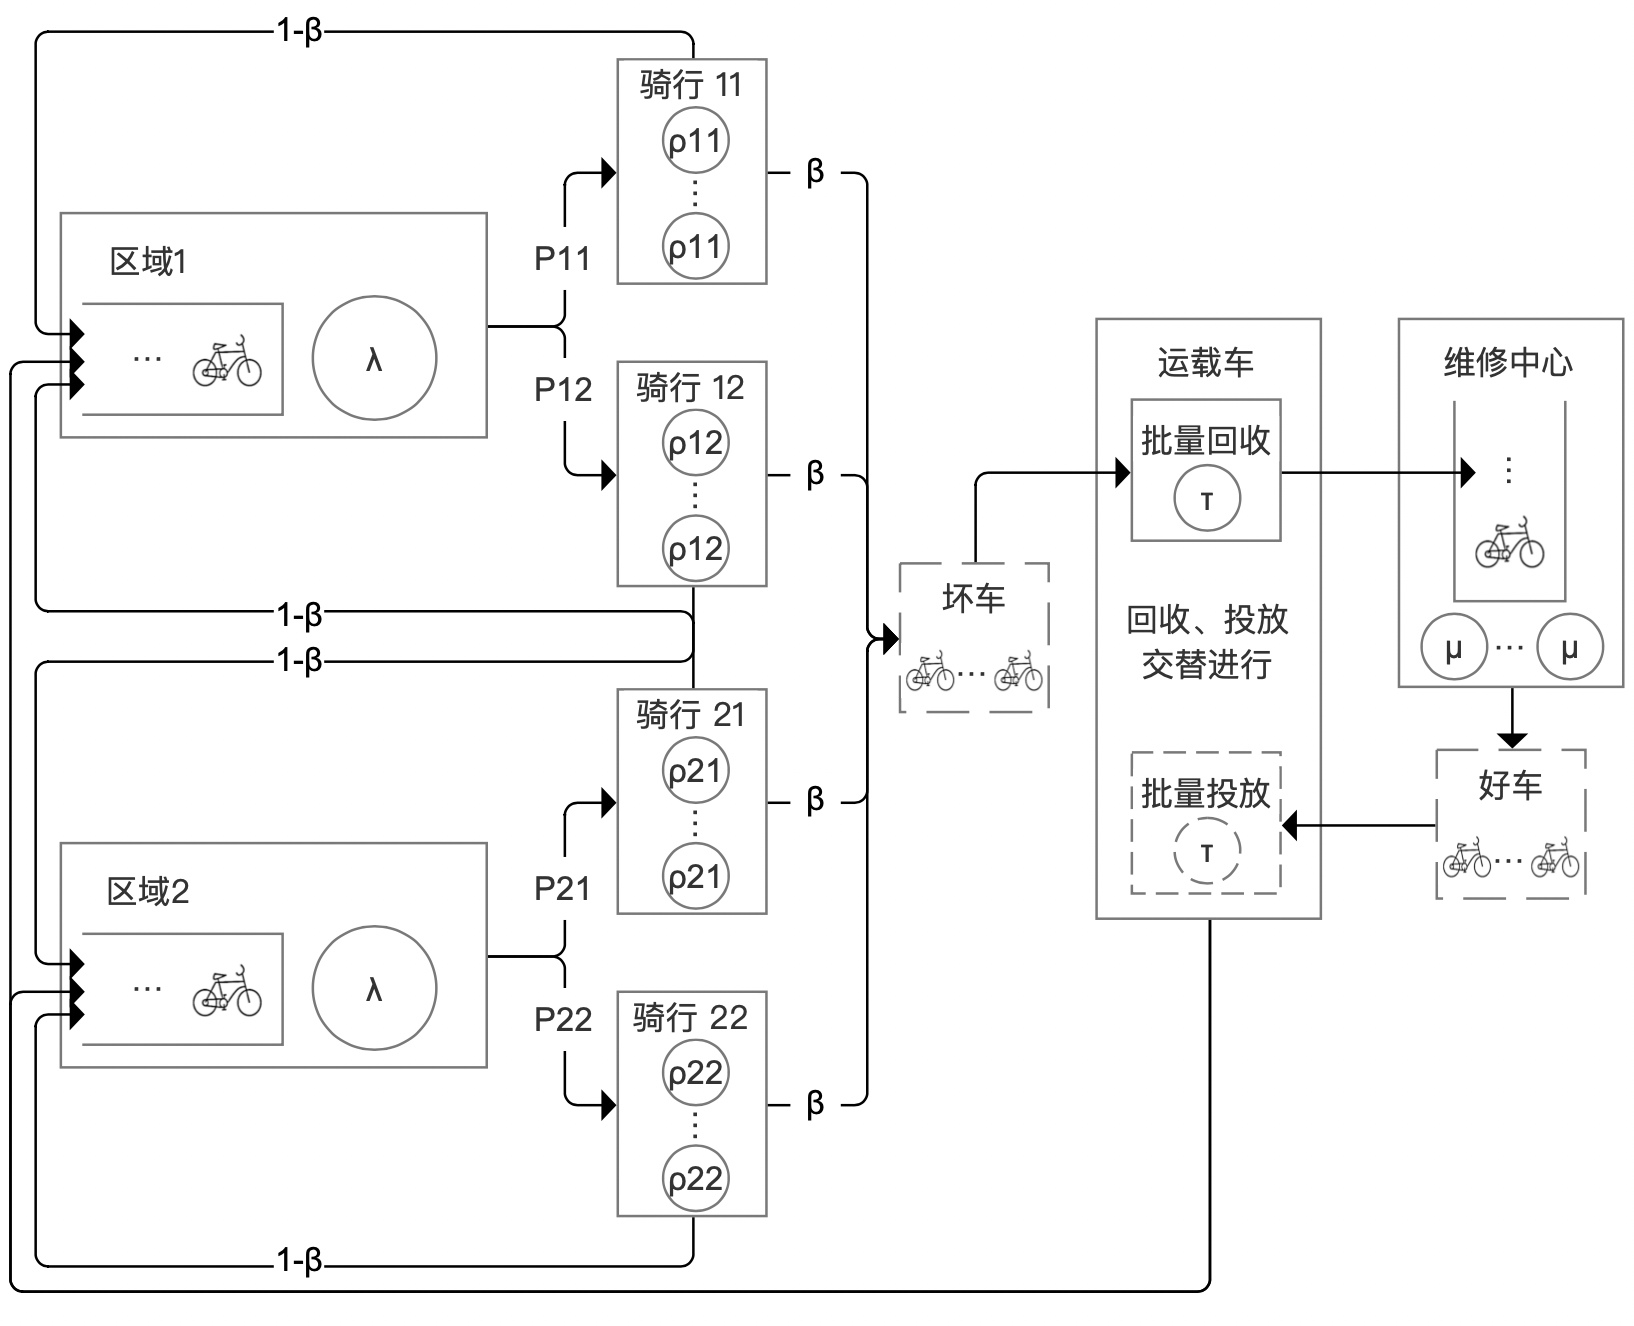
\includegraphics[scale=0.3]{./model/model.png}
    \caption{共享单车运维排队网络建模示意图}
    \label{fig:cenmodel}
\end{figure}


\subsection{符号标记}

\subsubsection{随机变量}
\begin{table}[H]
    \centering
    \caption{状态随机变量分量表}
    \begin{tabular}{ |c|c| } 
     \hline
     符号 & 含义 \\ 
     \hline
     $i, j$ & 队列的脚标, $i,j = 1, \dots, A$ \\ 
     \hline
     $t$ & 系统时间变量\\ 
     \hline
     $N_i$ & 在队列$i$处的好车数\\
     \hline
     $R_{ij}$ & 正在被从$i$骑到$j$的车数 \\ 
     \hline
     $BP$ & 当前等待被运送至维修中心的坏车数 \\
     \hline
     $RC$ & 当前维修队列处的坏车数 \\
    %  \hline
    %  $DP$ & 当前等待被重新投放的坏车数 \\
    %  \hline
    %  $OT$ & 当前运载车上的车辆数 \\
     \hline
     $I$ & 当前正在进行的投放或回收过程标记 \\
     \hline
    \end{tabular}
    \label{tab:rv}
\end{table}

\subsubsection{系统参数}
\begin{table}[H]
    \centering
    \caption{参数表}
    \begin{tabular}{ |c|c|c| } 
     \hline
     参数 & 描述 & 默认值 \\ 
     \hline
     $A$ & 区域数 & 2 \\ 
     \hline
     $M$ & 总车数 & 6 \\ 
     \hline
     $\beta$ & 损坏概率 & 0.3 \\
     \hline
     $P_{ij}$ & 从i到j的骑行概率 & 随机数 \\
     \hline
     $\lambda_i$ & 区域i顾客到达速率 & 随机数 \\
     \hline
     $\rho_{ij}$ & 从i骑行到j的速率 & i,j的曼哈顿距离加一的倒数 \\
     \hline
     $\tau$ & 运维速率 & 1.0 \\
     \hline
     $C$ & 运载车容量 & 3 \\
     \hline
     $\mu$ & 单服务台维修速率 & 1.0 \\
     \hline
     $N$ & 服务台数量 & 1.0 \\
     \hline
    \end{tabular}
    \label{tab:para}
\end{table}

\subsection{运维模型}
单车运维系统可以看成由好车服务和坏车运维两个部分组成。每个部分由若干排队队列组成,整体构成封闭排队网络。将在各队列中的自行车数作为状态向量的元素,我们使用$$\boldsymbol{X}_t = (N_1, \dots, N_{i}, \dots, N_A, R_{11}, \dots, R_{ij}, \dots, R_{AA}, BP, RC, DP)_t$$ 来表示系统在任意时间$t$的状态。
共享单车可以在各个区域中被骑行,从一个区域到达另一个区域或到达自身。骑行的时间根据区域间的距离不同,服从一定的指数分布。因而任意两个区域间相当于存在一个$M/M/\infty$队列。一次骑行完毕后,单车到达某个区域,进入这个区域的等待队列。每个区域的顾客到达服从一定参数的泊松分布。于是相当于可以服务的单车到达一个区域时进入一个$M/M/1$队列进行等待。当这个等待队列中没有单车时,新到达的顾客马上流失。当单车骑行完毕时也有可能进入损坏状态,此时其进入一个回收池\textit{Broken Pool}(简记为$BP$)。运载车负责将系统中损坏的单车回收运送至维修中心,和将维修中心处维修完毕的好车重新投放到运营之中。这里以\textit{Distribute Pool}(简记为$DP$),表示待投放的单车数量。运维车的操作时间服从参数为$\tau$的指数分布。也即,每隔一个参数为$\tau$的指数分布时间,运维车会搬运运载能力以内的尽可能多的坏车转移至维修中心,之后再经过参数为$\tau$的指数分布时间,维修后的好车被重新通入运营,这两个过程交替反复进行。投放策略本身是一个重要的、值得研究,并且已经有很多研究的问题【引用文献】。在本文中不作为重点讨论对象。为简化问题,转而采用一种较固定的可行策略:根据各个区域的顾客到达率和单车总数设置各个区域的目标数量,之后的投放以此为目标数量。需要注意的是,%为了模型的精简,这里的回收和重新投放过程,对现实中的操作进行了简化和抽象。只为了抓住批量化回收的特征和用参数去刻画回收和投放的能力强弱。由以上我们可以将共享单车的整体运维过程构建成一个排队网络。
由于每个队列处的服务时间的马尔可夫性,系统状态整体是一个连续时间马尔可夫链(Continuous-Time Markov Chain, CTMC)。因为好车可以以一定概率在任意区域之间被骑行,损坏了的车,将在维修后重新投放至各区域。显然系统中任意一个状态可以以一定概率经过一定时间后转移到任意另一个状态,因此这是一个遍历(Ergotic)的马尔可夫链。由马尔可夫链的性质,系统存在长程稳定状态。由此,我们可以计算得到一定系统参数设置下,系统处于各个状态的比率,进一步得到系统运行指标。


\section{模型求解}
对于一个遍历的连续时间马尔可夫链,当时间趋向于无穷大时,系统处于各个状态的比例趋向于一个固定值。该值服从系统的稳态概率转移方程。本部分我们构建系统的状态转移概率方程,并给出性能指标计算公式。但是这种方式很快会碰到系统状态数指数爆炸的情况,【状态数量计算公式】计算机内存难以存储如此大量的状态数。与此同时,多元线性方程组也难以求得精确解,从而无法获得系统较为准确的性能参数。而不能在较贴近实际的问题规模上进行求解。而仿真的方法计算系统的性能参数,可以较快收敛。因此,我们提出离散事件仿真的方法,得到系统的性能参数。

\subsection{方程构建}
记$S$为系统所有可能的状态的集合, $s$为集合中元素。记$$s^{T} = (N_1, \dots, N_A, R_{11}, \dots, R_{AA}, BP, RC, DP, I)^{T}$$为系统状态向量。对任意系统长程稳定状态其转出率与转入率相等。因为系统中的总的车数固定,所以其符合下式:
\begin{equation}
    \left\{
        \begin{array}{lcl}
            \sum \limits \limits _{i \in [1,A]}(N_i+\sum \limits _{j \in [1,A]}R_{ij})+BP+RC+DP = M; \\
            N_i, R_{ij}, BP, RC, DP\mbox{为}[0,M]\mbox{间的正整数}.
        \end{array}
    \right .
\end{equation}
\begin{equation}
    I = \left\{
        \begin{array}{lcl}
            0, &\mbox{坏车搬运} \\
            1, &\mbox{好车投放}.
        \end{array}
    \right .
\end{equation}

记$\pi_s$为状态$s$的极限稳态概率。我们记$I_{N_i}$,$I_{BP}$和$I_{DP}$如下:
\begin{equation}
I_{N_i}=\left\{
    \begin{array}{lcl}
        1, &N_i > 0;\\
        0, &\mbox{否则}.
    \end{array}    
\right.
\end{equation}
% \begin{equation}
% I_{Operation}=\left\{
%     \begin{array}{lcl}
%         1, &I=0\mbox{且}BP>0 \mbox{或} I=1\mbox{且}DP>0;\\
%         0, &\mbox{否则}.
%     \end{array}    
% \right.
% \end{equation}


由马尔可夫链的性质,系统稳态下任意状态的转出速率为该状态可以到达的任意下一状态的长程比例乘以相应转移速率之和。即:
\begin{equation}
Rate-out_{s} = (\sum \limits _{i \in [1,A]}\lambda_i I_{N_i}+\sum \limits _{i \in [1,A]} \sum \limits _{j \in [1,A]} \rho_{ij} R_{ij}+\lambda +\mu \min \{RC, N\} + \tau )\pi_s.
\end{equation}
我们记示性函数$I_{s^{'}}$如下,其表示一个状态是否是可能存在的,存在为1,不存在为0.
\begin{equation}
I_{s^{'}}=
    \left\{
        \begin{array}{lcl}
            1, &\sum \limits _{i \in [1,A]}(N_i+\sum \limits _{j \in [1,A]}R_{ij})+BP+RC+DP= M;\\ & N_i, R_{ij}, BP, RC, DP\mbox{为}[0,M]\mbox{间的正整数};\\
            0, &\mbox{否则}.
        \end{array}
    \right .  
\end{equation}
同样由马尔可夫链的性质,系统稳态下任意状态的转入速率为任意可以到达该状态的上一状态的长程比例乘以相应转移速率之和。而投放前各区域的好车数需要由投放策略倒推得到。本文中采取根据各区域顾客到达率按比例分配的策略。初始目标投放量根据每个区域的到达速率按比例进行设置。在每次投放时,按照每个区域的到达率从高到低排序,依次检查区域中当前的好车数是否达到原始设定的目标值,如果没有达到则尽可能补充到目标值。再投放下个区域。直到待投放的好车数为0或所有区域已检查过。根据这个策略可以得到所有可能的投放前系统状态集合$Q$。

则马尔可夫过程稳态情况下任意系统状态,可能由另一个状态经由(1)顾客骑走一辆好车;(2)骑行到达;(3)骑行损坏;(4)坏车运送至维修中心;(5)维修完毕进入投放队列;(6)投放至各区域,这六种过程的某一种而进入。从而确定系统某状态的转入速率为:
\begin{equation}
    \begin{aligned}
        Rate-in_{s} &= 
        \sum \limits _{i \in [1,A]} \sum \limits _{j \in [1,A]} \lambda_i P_{ij} \pi_{(\dots, N_i+1, \dots ,R_{ij}-1,\dots)} I_{(\dots, N_i+1, \dots ,R_{ij}-1,\dots)}\\
        &+\sum \limits _{i \in [1,A]} \sum \limits _{j \in [1,A]} \rho_{ji} R_{ji} (1-\beta) \pi_{(\dots, N_i-1, \dots ,R_{ij}+1,\dots)} I_{(\dots, N_i-1, \dots ,R_{ij}+1,\dots)}\\
        &+\sum \limits _{i \in [1,A]} \sum \limits _{j \in [1,A]} \rho_{ij} R_{ij} \beta \pi_{(\dots ,R_{ij}+1, \dots, \dots, BP-1, \dots)} I_{(\dots ,R_{ij}+1, \dots, \dots, BP-1, \dots)}\\
        &+\tau \sum \limits _{B \in [1,\min\{C, RC\}] } \pi_{(\dots, BP+B, RC-B, \dots, I=1)} \\
        &+\mu \min \{RC, N\} \pi_{(\dots, RC+1, DP-1)} I_{(\dots, RC+1, DP-1)}\\
        &+\tau \sum \limits _{q \in Q}\pi_{q} I_{q}\\
    \end{aligned}
\end{equation}
又有:
\begin{equation}
    \sum \limits _{s \in S} \pi_{s} = 1
\end{equation}
通过联立、求解以上系统状态转移概率方程组可以得到系统处于每个状态的长程比例。根据该比例可以计算得到系统平稳状态下的参数期望值。

\subsection{系统运行指标计算}
根据系统的长程稳态概率,也即系统处于每个状态的期望比例,可以计算得到一些我们关心的系统指标。
\subsubsection{期望好车、坏车比例}
系统中好车和坏车的比例可以由任意状态中的好车数量占车总数的比例求期望平均得到。
\begin{equation}
    E[\mbox{好车比例}] = \frac{1}{M} \sum \limits _{s \in S} \pi_{s} \sum \limits _{N_i \in s} N_i 
\end{equation}
\begin{equation}
    E[\mbox{坏车比例}] = 1 - E[\mbox{好车比例}]
\end{equation}

\subsubsection{期望顾客损失率}
当系统中某个区域处没有好车时,新到达的顾客将会损失掉。因此通过没有好车的区域的顾客到达速率除以总的顾客到达速率可以得到期望任意状态的顾客损失比率例。再通过对所有状态加权平均即可得到期望顾客损失率。
\begin{equation}
E[\mbox{顾客损失率}] = \frac{1}{M} \sum \limits _{s \in S} \pi_{s} \sum \limits _{N_i \in s} I(N_i) \lambda_i / \sum \limits _{i \in [1,A]} \lambda_i 
\end{equation}

\subsubsection{期望维修服务台闲置率}
维修中心处可能会有多台服务台。当维修中心处待维修的单车数少于维修台数量时,即出现了服务台的闲置。因此通过维修中心处的车数除以服务台数得到某一状态的限制比例,再通过对所有状态平均,即可得到期望维修服务台闲置率。
\begin{equation}
E[\mbox{维修服务台空置率}] = \sum \limits _{s \in S} \pi_{s} (1 - RC^s / N)
\end{equation}

% \subsubsection{期望回收、维修、投放车数比例}
% 期望回收、维修、投放车数比例即为回收、维修、投放三个队列的期望车数。与前述好车比例的计算类似。
% \begin{equation}
% E[\mbox{BP比例}] = \frac{1}{M} \sum \limits _{s \in S} \pi_{s} BP^s 
% \end{equation}
% \begin{equation}
% E[\mbox{RC比例}] = \frac{1}{M} \sum \limits _{s \in S} \pi_{s} RC^s 
% \end{equation}
% \begin{equation}
% E[\mbox{DP比例}] = \frac{1}{M} \sum \limits _{s \in S} \pi_{s} DP^s 
% \end{equation}

\subsection{仿真方法}
离散事件系统仿真方法,可以通过生成符合分布假设的随机数,完整模拟所建立的模型对应的系统的运行。通过记录系统运行中的参数变化,可以直接获得系统的性能参数。并且当系统存在大量状态时,其中很多的稳态被访问比例是十分低的。但是仿真系统可以很快进入稳定状态,从而无需记录系统处于所有状态的比例。因而基于仿真的方法可以较快地得到系统的性能参数。通过设置同样的系统参数,对照方程求解结果和仿真结果,也可以验证CTMC模型ODE方程求解方法与仿真方法的正确性。

\subsubsection{仿真的稳态}
首先通过离散系统仿真的方法,给系统设置如表\ref{tab:rv}和\ref{tab:para}所示的默认系统参数。初始系统中所有车均为可骑状态,并且平均分布于各个区域中。通过记录系统中好车数量、到达顾客数量、损失顾客数量和维修中心是否闲置这几个系统状态,及这些状态在系统中持续的时间,计算得到系统中期望好车比例、期望顾客损失比例和期望维修中心闲置比例。通过观察这些指标随仿真系统时间的变化,判断系统是否进入稳态,取系统【引用系统仿真时间的设置】稳态的状态。并以此时间作为其他仿真测试的时间标准,在不严重影响程序性能,而导致时间无法接受的前提下,尽可能延长仿真的时间,获得期望的系统性能参数。示例如下。
\begin{figure}[H]
    \centering
    \includegraphics[scale=0.5]{sim/A10M50系统性能参数-时间40000图.png}
    \caption{A10M50系统性能参数-时间40000图}
    \label{fig:cenmodel}
\end{figure}

\subsubsection{性能参数验证}
通过设置相同的参数比较,方程求解结果与仿真结果。如下图所示:
\begin{figure}[H]
    \centering
    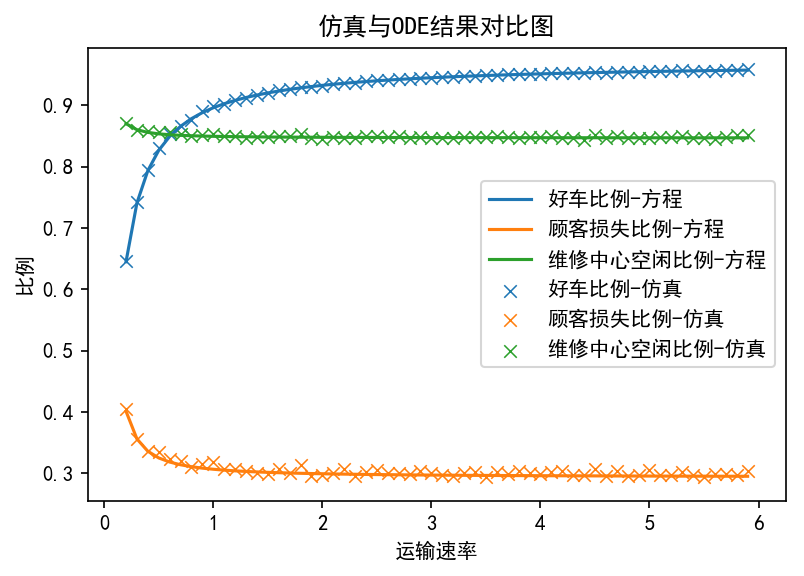
\includegraphics[scale=0.5]{A2M6仿真-odeSingle.png}
    \caption{A2M6方程与仿真结果对比图}
    \label{fig:cenmodel}
\end{figure}

\subsection{运维决策}
在单车的日常运营中需要确定采用多少运载能力和维修能力。现实中,往往有不同运载量的运载工具进行选择,有运载量很小的电动三轮车,也有运载量适中的箱式货车,还有运载量比较大的卡车。运维中心需要多少维修工人,也是一个需要考虑的问题。基于前述建模的系统性能参数仍难以进行显式的表达,也因而难以直接作为目标函数进行优化。但是通过仿真的方法,可以较方便地获得系统性能参数。通过对前述仿真模型的简单扩展,可以仿真有多种运载车同时运行的情况。在本文中为了模型的简洁,同一种类的多辆运载车表示为服务速率的成倍增加。系统中可分配到运载车和维修人员的资源预算为给定的有限值。不同运载量运载工具的单位平均成本,单位维修人员的成本也作为默认值给定。
目标函数为最小化系统中顾客损失。对应的变量如表所示。
\begin{table}[H]
    \centering
    \caption{决策问题相关变量表}
    \begin{tabular}{ |c|c| } 
     \hline
     符号 & 含义 \\ 
     \hline
     $V$ & 运载工具种类数, 正整数 \\ 
     \hline
     $v$ & 运载工具种类的脚标, $v= 1, \dots, V$ \\ 
     \hline
     $n_v$ & 决策变量,运载工具$v$的数量,自然数\\ 
     \hline
     $N$ & 决策变量,维修服务台的数量,自然数\\ 
     \hline
     $cost_v$ & 运载工具$v$的单位成本\\ 
     \hline
     $cost_{RC}$ & 维修台的单位成本\\
     \hline
     $T$ & 预算总数 \\ 
    %  \hline
    %  $DP$ & 当前等待被重新投放的坏车数 \\
    %  \hline
    %  $OT$ & 当前运载车上的车辆数 \\
     \hline
    \end{tabular}
    \label{tab:rv}
\end{table}
需要求解的问题如下:
% \begin{align*}
%     \min \quad & \mathbb{E}[顾客损失比例] & \tag{1}\\
%     \mbox{s.t.}\quad
%     &\Sigma  \limits _{v \in V} n_v cost_v + N \quad cost_{RC} <= T,  & \tag{2}\\
%     &n_v \in \mathbb{N} &\tag{3}\\
% \end{align*}
\begin{align*}
    &\min \quad \mathbb{E}[\mbox{顾客损失比例}]\\
    & \begin{array}{r@{\quad}r@{}l@{\quad}l}
    s.t.&\sum \limits _{v \in V} n_v cost_v + N cost_{RC}&\leq T\\
     &n_v, N&\in\mathbb{N}\\
    \end{array} 
\end{align*}
由于系统的随机性和不能显式描述的特性我们采用仿真优化的方法。本优化问题的决策变量为离散值。决策空间随着运载车的种类和预算的增加而呈指数增加,难以进行遍历。因此本部分采用模拟退火算法,搜索系统的最优决策。

\begin{table}[H]
    \centering
    \caption{决策问题参数设置表}
    \begin{tabular}{ |c|c| } 
     \hline
     参数 & 取值 \\ 
     \hline
     $A$ & 10 \\ 
     \hline
     $M$ & 200 \\ 
     \hline
     $V$ & 5 \\ 
     \hline
     $Capacity_v$ & [1,5,10,20,50] \\ 
     \hline
     $Cost_v$ & [1,2,3,4,5]\\ 
     \hline
     $Cost_{RC}$ & 1 \\
     \hline
     $T$ & 10 \\ 
     \hline
    \end{tabular}
    \label{tab:rv}
\end{table}

\section{算例分析}
\newpage

% \section{运维过程建模}
% 共享单车的有桩无桩模式相较有桩模式而言,单车的分布情况是比较散乱的。而在实际中,单车的运维往往是基于划分的区域进行的。为了研究方便,本工作将共享单车的运行区域抽象成一个个相邻的区域。加上单车的运维部分,整体构成共享单车的运行系统。如图\ref{fig:cenmodel}所示。通常情况下,共享单车采用集中式维修的模式。在该模式下,操作员使用运输工具将一定区域内无法使用的自行车收集起来进行集中维修。一些工人在维修中心维修后仍无法使用的自行车将被替换成新车。然后,维修好的自行车将被重新分配到各个区域。这样的过程一致持续进行。通常在日常运行中还有一项工作是,搬运各个区域中分布的好车,以使各个区域中的可使用的单车数量尽可能满足该区域的骑行需求。因为通常现实中单车的调度也不是持续不断的进行的,而是隔一段时间进行,或者夜间进行,在调度过程中可以看做是不受控制的运行。或者根据实际运行情况,某个区域当前或者预期需求持续得不到满足,而需要往这个区域调配车辆。在本文中,不是重点的讨论的对象。因此,只在单车重新投放时考虑根据各个区域的顾客到达速率进行按比例分配。本文构建了一个封闭排队网络研究该服务系统。

% \begin{figure}[H]
%     \centering
%     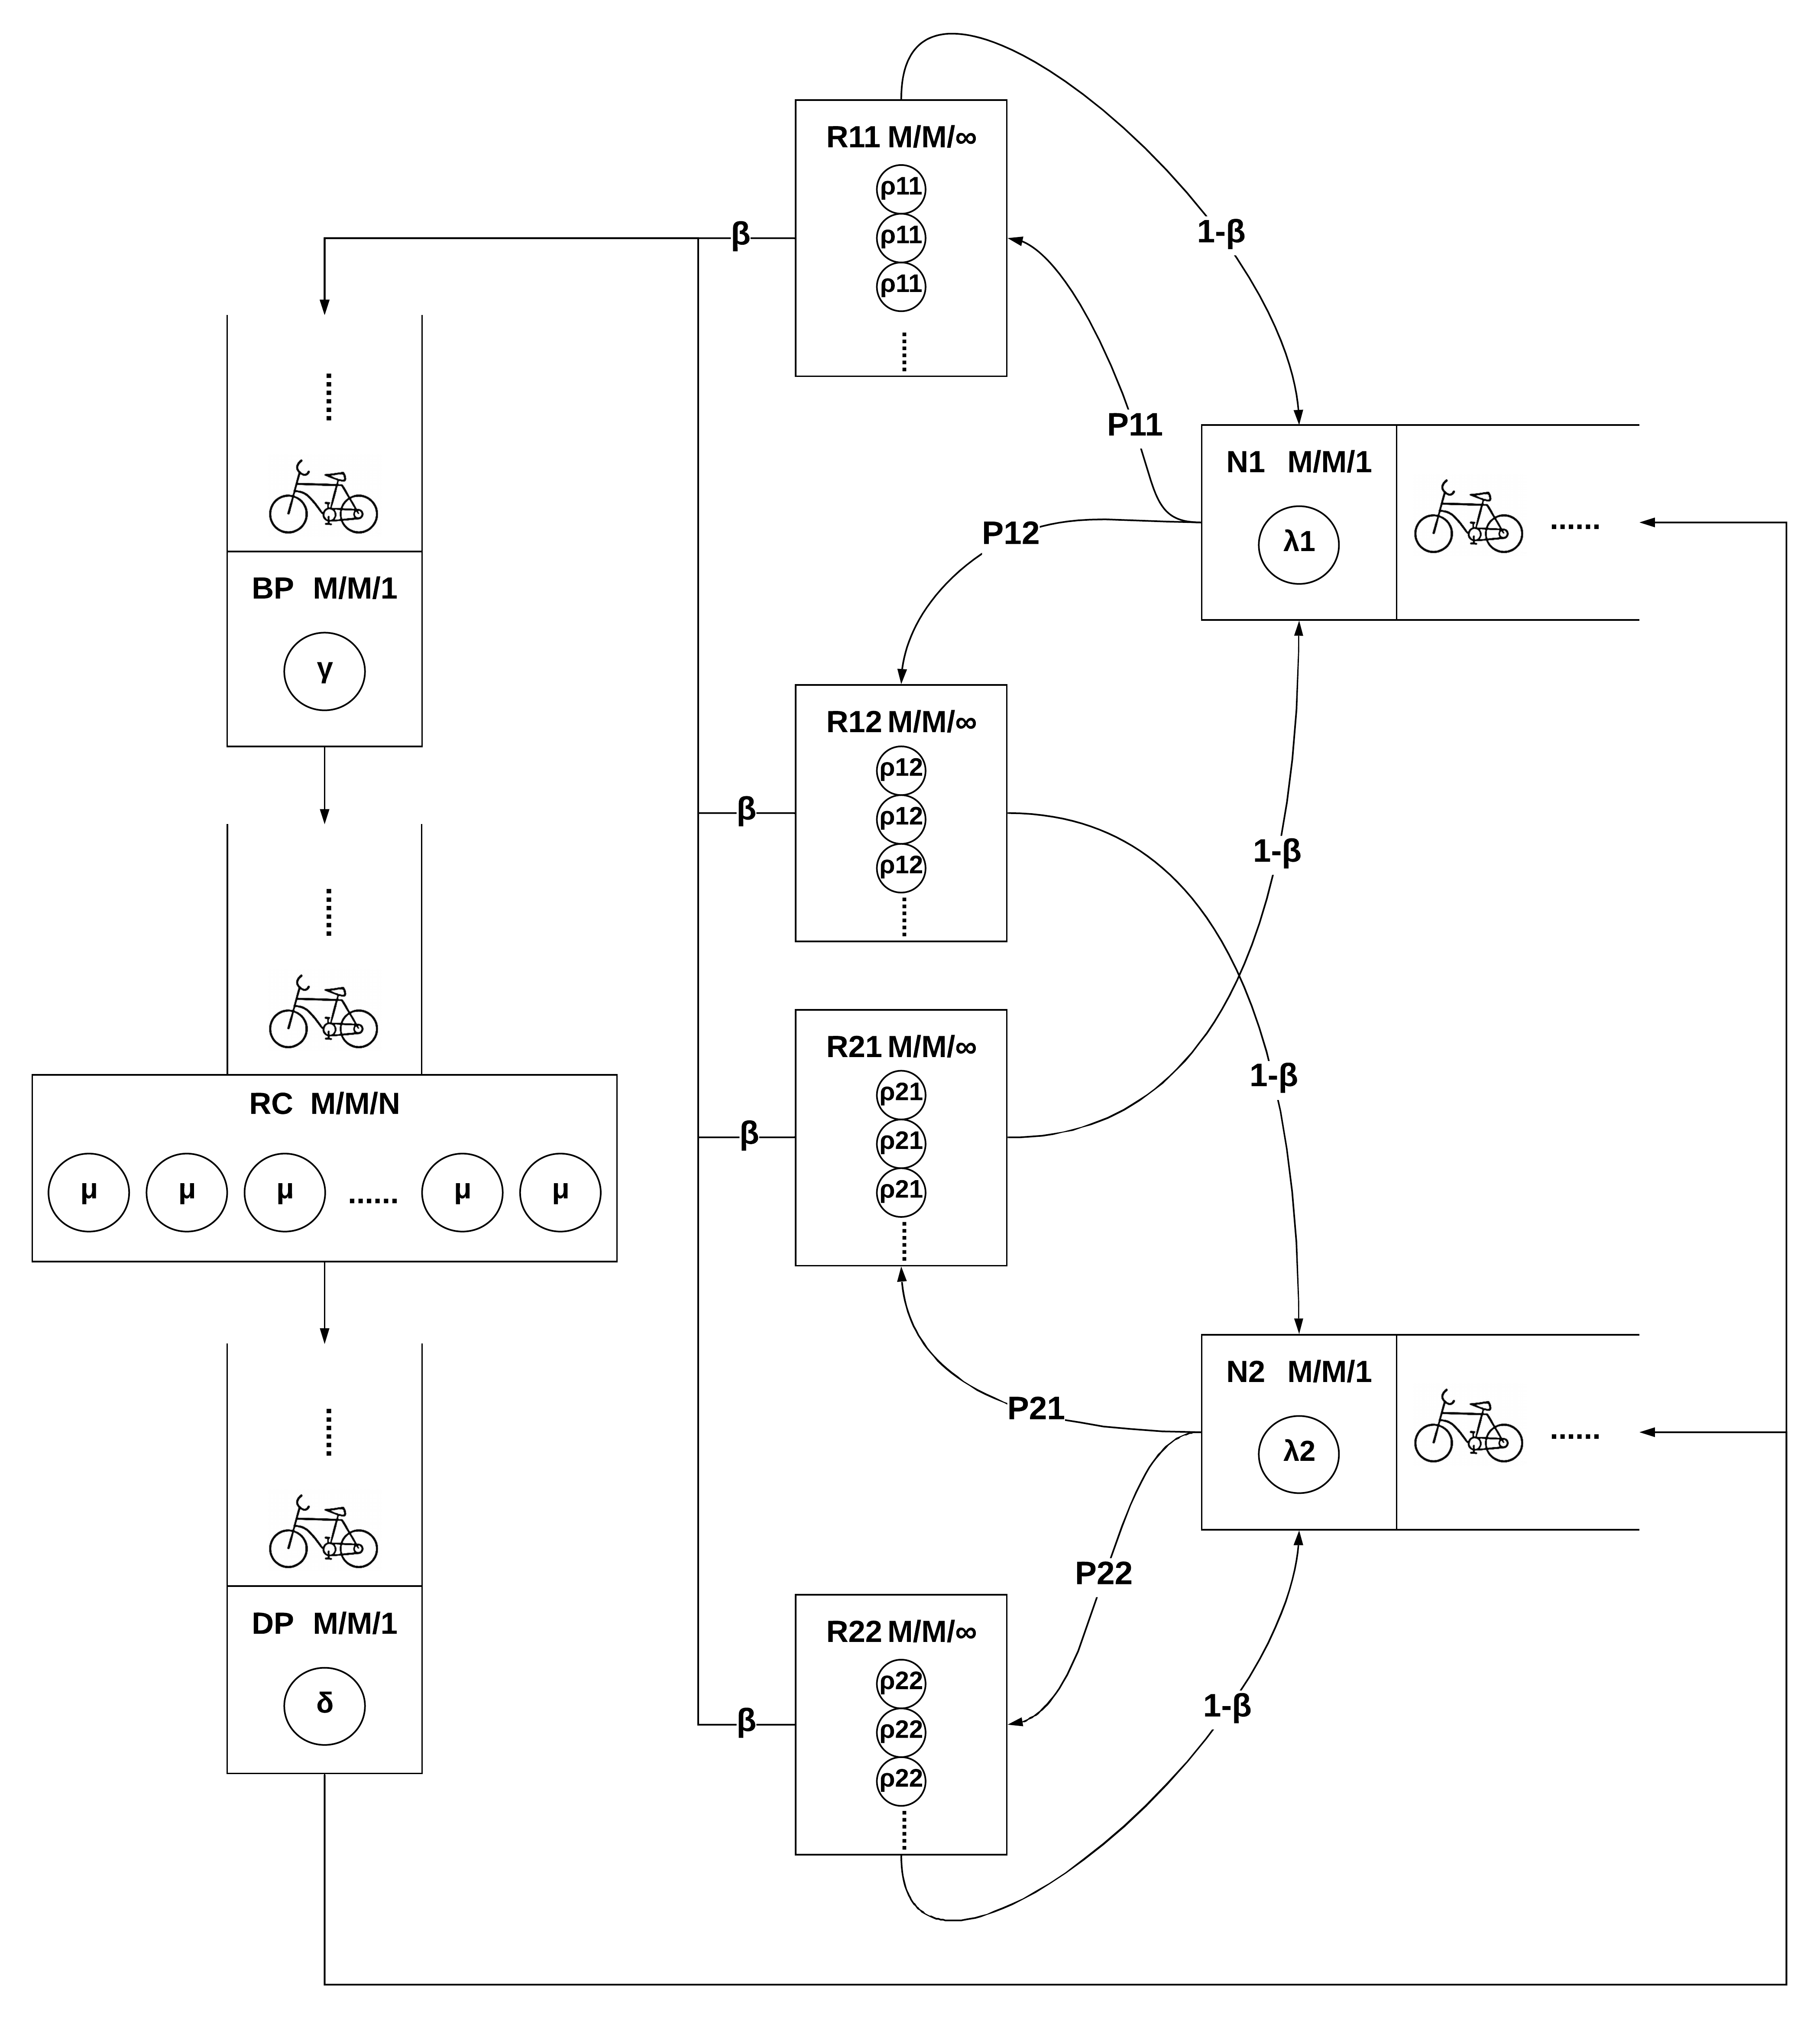
\includegraphics[scale=0.3]{CentralModel2.png}
%     \caption{共享单车运维排队网络建模示意图}
%     \label{fig:cenmodel}
% \end{figure}


% \subsection{符号标记}

% \subsubsection{随机变量}
% \begin{table}[H]
%     \centering
%     \caption{状态随机变量分量表}
%     \begin{tabular}{ |c|c| } 
%      \hline
%      符号 & 含义 \\ 
%      \hline
%      $i, j$ & 队列的脚标, $i,j = 1, \dots, A$ \\ 
%      \hline
%      $t$ & 系统时间变量\\ 
%      \hline
%      $N_i$ & 在队列$i$处的好车数\\
%      \hline
%      $R_{ij}$ & 正在被从$i$骑到$j$的车数 \\ 
%      \hline
%      $BP$ & 当前等待被运送至维修中心的坏车数 \\
%      \hline
%      $RC$ & 当前维修队列处的坏车数 \\
%      \hline
%      $DP$ & 当前等待被重新投放的坏车数 \\
%      \hline
%     \end{tabular}
%     \label{rv}
% \end{table}

% \subsubsection{系统参数}
% \begin{table}[H]
%     \centering
%     \caption{参数表}
%     \begin{tabular}{ |c|c|c| } 
%      \hline
%      参数 & 描述 & 默认值 \\ 
%      \hline
%      $A$ & 区域数 & 2 \\ 
%      \hline
%      $M$ & 总车数 & 6 \\ 
%      \hline
%      $\beta$ & 损坏概率 & 0.3 \\
%      \hline
%      $P_{ij}$ & 从i到j的骑行概率 & 随机数 \\
%      \hline
%      $\lambda_i$ & 区域i顾客到达速率 & 随机数 \\
%      \hline
%      $\rho_{ij}$ & 从i骑行到j的速率 & i,j的曼哈顿距离加一的倒数 \\
%      \hline
%      $\gamma$ & 回收速率 & 1.0 \\
%      \hline
%      $\overline{B}$ & 回收批量 & 1 \\
%      \hline
%      $\mu$ & 单服务台维修速率 & 1.0 \\
%      \hline
%      $N$ & 服务台数量 & 1 \\
%      \hline
%      $\delta$ & 投放速率 & 1.0 \\
%      \hline
%      $\overline{D}$ & 投放批量 & 2 \\
%      \hline
%     \end{tabular}
%     \label{para}
% \end{table}

% \subsection{运维模型}
% 单车运维系统可以看成由好车服务和坏车运维两个部分组成。每个部分由若干排队队列组成,整体构成封闭排队网络。将在各队列中的自行车数作为状态向量的元素,我们使用$$\boldsymbol{X}_t = (N_1, \dots, N_{i}, \dots, N_A, R_{11}, \dots, R_{ij}, \dots, R_{AA}, BP, RC, DP)_t$$ 来表示系统在任意时间$t$的状态。
% 共享单车可以在各个区域中被骑行,从一个区域到达另一个区域或到达自身。骑行的时间根据区域间的距离不同,服从一定的指数分布。因而任意两个区域间相当于存在一个$M/M/\infty$队列。一次骑行完毕后,单车到达某个区域,进入这个区域的等待队列。每个区域的顾客到达服从一定参数的泊松分布。于是相当于可以服务的单车到达一个区域时进入一个$M/M/1$队列进行等待。当这个等待队列中没有单车时,新到达的顾客马上流失。当单车骑行完毕时也有可能进入损坏状态,此时其进入一个回收池\textit{Broken Pool}(简记为$BP$)。当回收池中的坏车数量达到一定阈值$\overline{B}$,或者系统中已经没有好车,而回收池中有车时,这批坏车经过参数为$\gamma$指数时间后到达维修中心\textit{Repairing Center}(简记为$RC$)。维修中心处的维修过程相当于$M/M/N$的排队过程。有$N$个服务台负责对单车进行维修,每个服务台的维修时间服从相同的指数分布。当单车维修完毕后,随即进入一个投放池\textit{Distribute Pool}(简记为$DP$)。当该处的好车数达到一定阈值$\overline{D}$,或者系统中已经没有好车,而投放池中有车时,这些车经过参数为$\delta$的指数时间后,重新投放至各个区域。投放策略本身是一个重要的、值得研究,并且已经有很多研究的问题。在本文中不作为重点讨论对象。本文采用一种较基本的策略:根据各个区域的顾客到达率和单车总数设置各个区域的目标数量,之后的投放以此为目标数量。需要注意的是,为了模型的精简,这里的回收和重新投放过程,对现实中的操作进行了简化和抽象。只为了抓住批量化回收的特征和用参数去刻画回收和投放的能力强弱。由以上我们可以将共享单车的整体运维过程构建成一个排队网络。
% 由于每个队列处的服务时间的马尔可夫性,系统状态整体是一个连续时间马尔可夫链(Continuous-Time Markov Chain, CTMC)。因为好车可以以一定概率在任意区域之间被骑行,损坏了的车,将在维修后重新投放至各区域。显然系统中任意一个状态可以以一定概率经过一定时间后转移到任意另一个状态,因此这是一个遍历(Ergotic)的马尔可夫链。由马尔可夫链的性质,系统存在长程稳定状态。由此,我们可以计算得到一定系统参数设置下,系统处于各个状态的比率,进一步得到系统运行指标。


% \section{模型求解}
% 对于一个遍历的连续时间马尔可夫链,当时间趋向于无穷大时,系统处于各个状态的比例趋向于一个固定值。该值服从系统的稳态概率转移方程。本部分我们构建系统的状态转移概率方程,并给出性能指标计算公式。

% \subsection{方程构建}
% 记$S$为系统所有可能的状态的集合, $s$为集合中元素。记$$s^{T} = (N_1, \dots, N_A, R_{11}, \dots, R_{AA}, BP, RC, DP)^{T}$$为系统状态向量。对任意系统长程稳定状态其转出率与转入率相等。因为系统中的总的车数固定,所以其符合下式:
% \begin{equation}
%     \left\{
%         \begin{array}{lcl}
%             \sum \limits \limits _{i \in [1,A]}(N_i+\sum \limits _{j \in [1,A]}R_{ij})+BP+RC+DP = M; \\
%             N_i, R_{ij}, BP, RC, DP\mbox{为}[0,M]\mbox{间的正整数}.
%         \end{array}
%     \right .
% \end{equation}

% 记$\pi_s$为状态$s$的极限稳态概率。我们记$I_{N_i}$,$I_{BP}$和$I_{DP}$如下:
% \begin{equation}
% I_{N_i}=\left\{
%     \begin{array}{lcl}
%         1, &N_i > 0;\\
%         0, &\mbox{否则}.
%     \end{array}    
% \right.
% \end{equation}
% \begin{equation}
% I_{BP}=\left\{
%     \begin{array}{lcl}
%         1, &BP \geq \overline{B} \quad \mbox{或} BP + RC + DP = M \land BP \neq 0;\\
%         0, &\mbox{否则}.
%     \end{array}    
% \right.
% \end{equation}
% \begin{equation}
% I_{DP}=\left\{
%     \begin{array}{lcl}
%         1, &DP \geq \overline{D} \quad \mbox{或} BP + RC + DP = M \land DP \neq 0;\\
%         0, &\mbox{否则}.
%     \end{array}    
% \right.
% \end{equation}

% 由马尔可夫链的性质,系统稳态下任意状态的转出速率为该状态可以到达的任意下一状态的长程比例乘以相应转移速率之和。即:
% \begin{equation}
% Rate-out_{s} = (\sum \limits _{i \in [1,A]}\lambda_i I_{N_i}+\sum \limits _{i \in [1,A]} \sum \limits _{j \in [1,A]} \rho_{ij} R_{ij}+\gamma I_{BP} +\mu \min \{RC, N\}+\delta I_{DP} )\pi_s.
% \end{equation}
% 我们记示性函数$I_{s^{'}}$如下,其表示一个状态是否是可能存在的,存在为1,不存在为0.
% \begin{equation}
% I_{s^{'}}=
%     \left\{
%         \begin{array}{lcl}
%             1, &\sum \limits _{i \in [1,A]}(N_i+\sum \limits _{j \in [1,A]}R_{ij})+BP+RC+DP = M;\\ & N_i, R_{ij}, BP, RC, DP\mbox{为}[0,M]\mbox{间的正整数};\\
%             0, &\mbox{否则}.
%         \end{array}
%     \right .  
% \end{equation}
% 同样由马尔可夫链的性质,系统稳态下任意状态的转入速率为任意可以到达该状态的上一状态的长程比例乘以相应转移速率之和。为了确定任意状态的转入速率需要先给定回收和投放两个过程的可能状态变化量。
% 回收过程的变化量由下式给出。
% \begin{equation}
% B=\left\{
%     \begin{array}{lcl}
%         BP, & BP + RC + DP = M \land BP \neq 0;\\
%         \overline{B}, &\mbox{否则}.
%     \end{array}    
% \right.
% \end{equation}
% 每次待投放的数量由下式给出。
% \begin{equation}
% D=\left\{
%     \begin{array}{lcl}
%         DP, & BP + RC + DP = M \land DP \neq 0;\\
%         \overline{D}, &\mbox{否则}.
%     \end{array}    
% \right.
% \end{equation}
% 而投放前各区域的好车数需要由投放策略倒推得到。本文中采取根据各区域顾客到达率按比例分配的策略。初始目标投放量根据每个区域的到达速率按比例进行设置。在每次投放时,按照每个区域的到达率从高到低排序,依次检查区域中当前的好车数是否达到原始设定的目标值,如果没有达到则尽可能补充到目标值。再投放下个区域。直到待投放的好车数为0或所有区域已检查过。根据这个策略可以得到所有可能的投放前系统状态集合$Q$。

% 则马尔可夫过程稳态情况下任意系统状态,可能由另一个状态经由(1)顾客骑走一辆好车;(2)骑行到达;(3)骑行损坏;(4)坏车运送至维修中心;(5)维修完毕进入投放队列;(6)投放至各区域,这六种过程的某一种而进入。从而确定系统某状态的转入速率为:
% \begin{equation}
%     \begin{array}{lcl}
%         Rate-in_{s} = \\
%         \sum \limits _{i \in [1,A]} \sum \limits _{j \in [1,A]} \lambda_i P_{ij} \pi_{(\dots, N_i+1, \dots ,R_{ij}-1,\dots)} I_{(\dots, N_i+1, \dots ,R_{ij}-1,\dots)}+\\
%         \sum \limits _{i \in [1,A]} \sum \limits _{j \in [1,A]} \rho_{ji} R_{ji} (1-\beta) \pi_{(\dots, N_i-1, \dots ,R_{ij}+1,\dots)} I_{(\dots, N_i-1, \dots ,R_{ij}+1,\dots)}+\\
%         \sum \limits _{i \in [1,A]} \sum \limits _{j \in [1,A]} \rho_{ij} R_{ij} \beta \pi_{(\dots ,R_{ij}+1, \dots, \dots, BP-1, \dots)} I_{(\dots ,R_{ij}+1, \dots, \dots, BP-1, \dots)}+\\
%         \gamma \pi_{(\dots, BP+B, RC-B, \dots)} I_{(\dots, BP+B, RC-B, \dots)}+\\
%         \mu \min \{RC, N\} \pi_{(\dots, RC+1, DP-1)} I_{(\dots, RC+1, DP-1)}+\\
%         \delta \sum \limits _{q \in Q}\pi_{q} I_{q}\\
%     \end{array}
% \end{equation}
% 又有:
% \begin{equation}
%     \sum \limits _{s \in S} \pi_{s} = 1
% \end{equation}
% 通过联立、求解以上系统状态转移概率方程组可以得到系统处于每个状态的长程比例。根据该比例可以计算得到系统平稳状态下的参数期望值。

% \subsection{系统运行指标计算}
% 根据系统的长程稳态概率,也即系统处于每个状态的期望比例,可以计算得到一些我们关心的系统指标。
% \subsubsection{期望好车、坏车比例}
% 系统中好车和坏车的比例可以由任意状态中的好车数量占车总数的比例求期望平均得到。
% \begin{equation}
%     E[\mbox{好车比例}] = \frac{1}{M} \sum \limits _{s \in S} \pi_{s} \sum \limits _{N_i \in s} N_i 
% \end{equation}
% \begin{equation}
%     E[\mbox{坏车比例}] = 1 - E[\mbox{好车比例}]
% \end{equation}

% \subsubsection{期望顾客损失率}
% 当系统中某个区域处没有好车时,新到达的顾客将会损失掉。因此通过没有好车的区域的顾客到达速率除以总的顾客到达速率可以得到期望任意状态的顾客损失比率例。再通过对所有状态加权平均即可得到期望顾客损失率。
% \begin{equation}
% E[\mbox{顾客损失率}] = \frac{1}{M} \sum \limits _{s \in S} \pi_{s} \sum \limits _{N_i \in s} I(N_i) \lambda_i / \sum \limits _{i \in [1,A]} \lambda_i 
% \end{equation}

% \subsubsection{期望维修服务台闲置率}
% 维修中心处可能会有多台服务台。当维修中心处待维修的单车数少于维修台数量时,即出现了服务台的闲置。因此通过维修中心处的车数除以服务台数得到某一状态的限制比例,再通过对所有状态平均,即可得到期望维修服务台闲置率。
% \begin{equation}
% E[\mbox{维修服务台空置率}] = \sum \limits _{s \in S} \pi_{s} (1 - RC^s / N)
% \end{equation}

% \subsubsection{期望回收、维修、投放车数比例}
% 期望回收、维修、投放车数比例即为回收、维修、投放三个队列的期望车数。与前述好车比例的计算类似。
% \begin{equation}
% E[\mbox{BP比例}] = \frac{1}{M} \sum \limits _{s \in S} \pi_{s} BP^s 
% \end{equation}
% \begin{equation}
% E[\mbox{RC比例}] = \frac{1}{M} \sum \limits _{s \in S} \pi_{s} RC^s 
% \end{equation}
% \begin{equation}
% E[\mbox{DP比例}] = \frac{1}{M} \sum \limits _{s \in S} \pi_{s} DP^s 
% \end{equation}


% \section{数值实验}
% 本部分首先采用前述的系统参数计算方法,在设置的模型上进行小规模数值实验,研究单车运维系统中回收、维修和投放三个过程的参数变动,对整个系统的运行效果的影响。但是当问题规模扩大时,由于系统状态数以指数增长,因此稳态概率的计算难以进行,因此我们采用仿真的方法,在一个较大规模设置下进行了数值实验,观察在不同规模系统的运行规律。

% \subsection{参数设置}
% 在这一部分,我们保持系统中的区域数量、车的总数量、车向其他区域的转移概率和骑行速率固定,变动运维系统的参数。主要关注运维中的回收批量、回收速率、维修台数量、维修台速率、投放批量和投放速率这六个参数。基于前述公式,计算不同参数对应情况下的7个系统指标。这些指标分别是:平均好车比例、平均坏车比例、顾客损失率、维修中心闲置率、回收池平均队长、维修中心平均队长和投放池平均队长。观察参数变化引起的系统服务能力变化。在每一种参数设置情况中,每个区域的顾客到达率和区域之间的转移概率使用随机数发生器产生。通过在每种参数设置下运行30次不同的随机数实验,去除掉不同运行环境的影响。系统参数的默认值如表\ref{para}所示。


% 下图为500次随机概率转移和每个区域到达速率情况下的各系统参数情况。
% \begin{figure}[H]
%     \centering
%     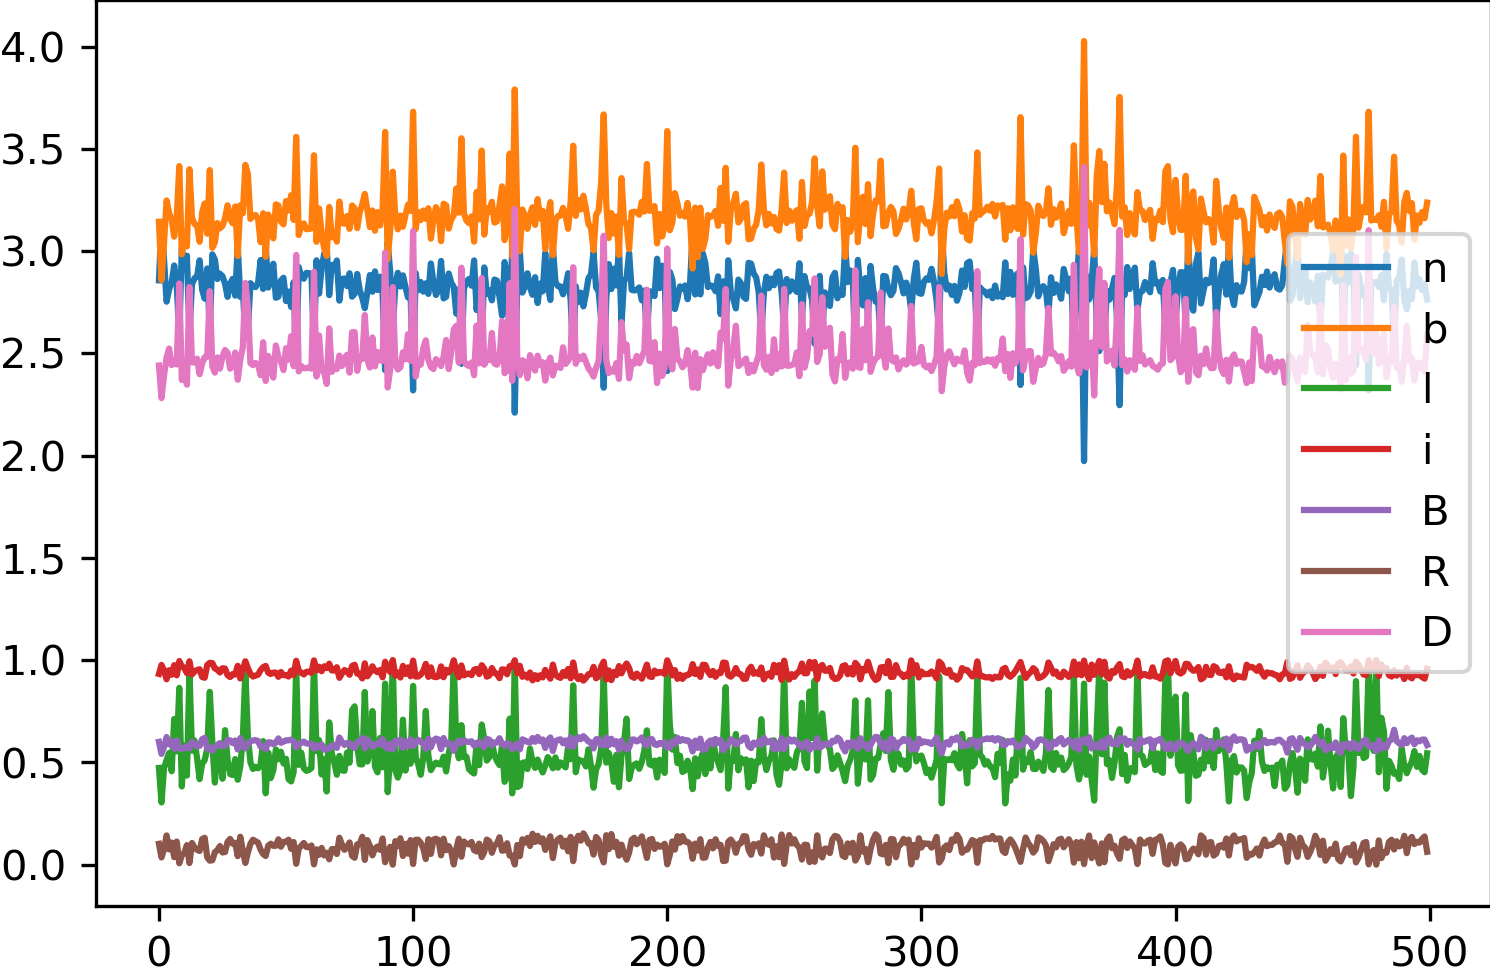
\includegraphics[scale=0.6]{/Graph/500epics.png}
%     \caption{500次随机环境结果}
%     \label{fig:cenAvgTime}
% \end{figure}
% 在不同概率转移和到达速率情况下,各系统参数分布在一定范围内。因此,在之后的实验中,我们在任意给定运维参数下,都将随机运行30次,以均值作为当前参数的结果。以过滤掉系统中骑行因素的影响。

% 为了确定系统参数,我们首先观察研究了随机情况下,单车损坏率与系统状态的关系。如图\ref{fig:betaRate}所示。
% \begin{figure}[H]
%     \centering
%     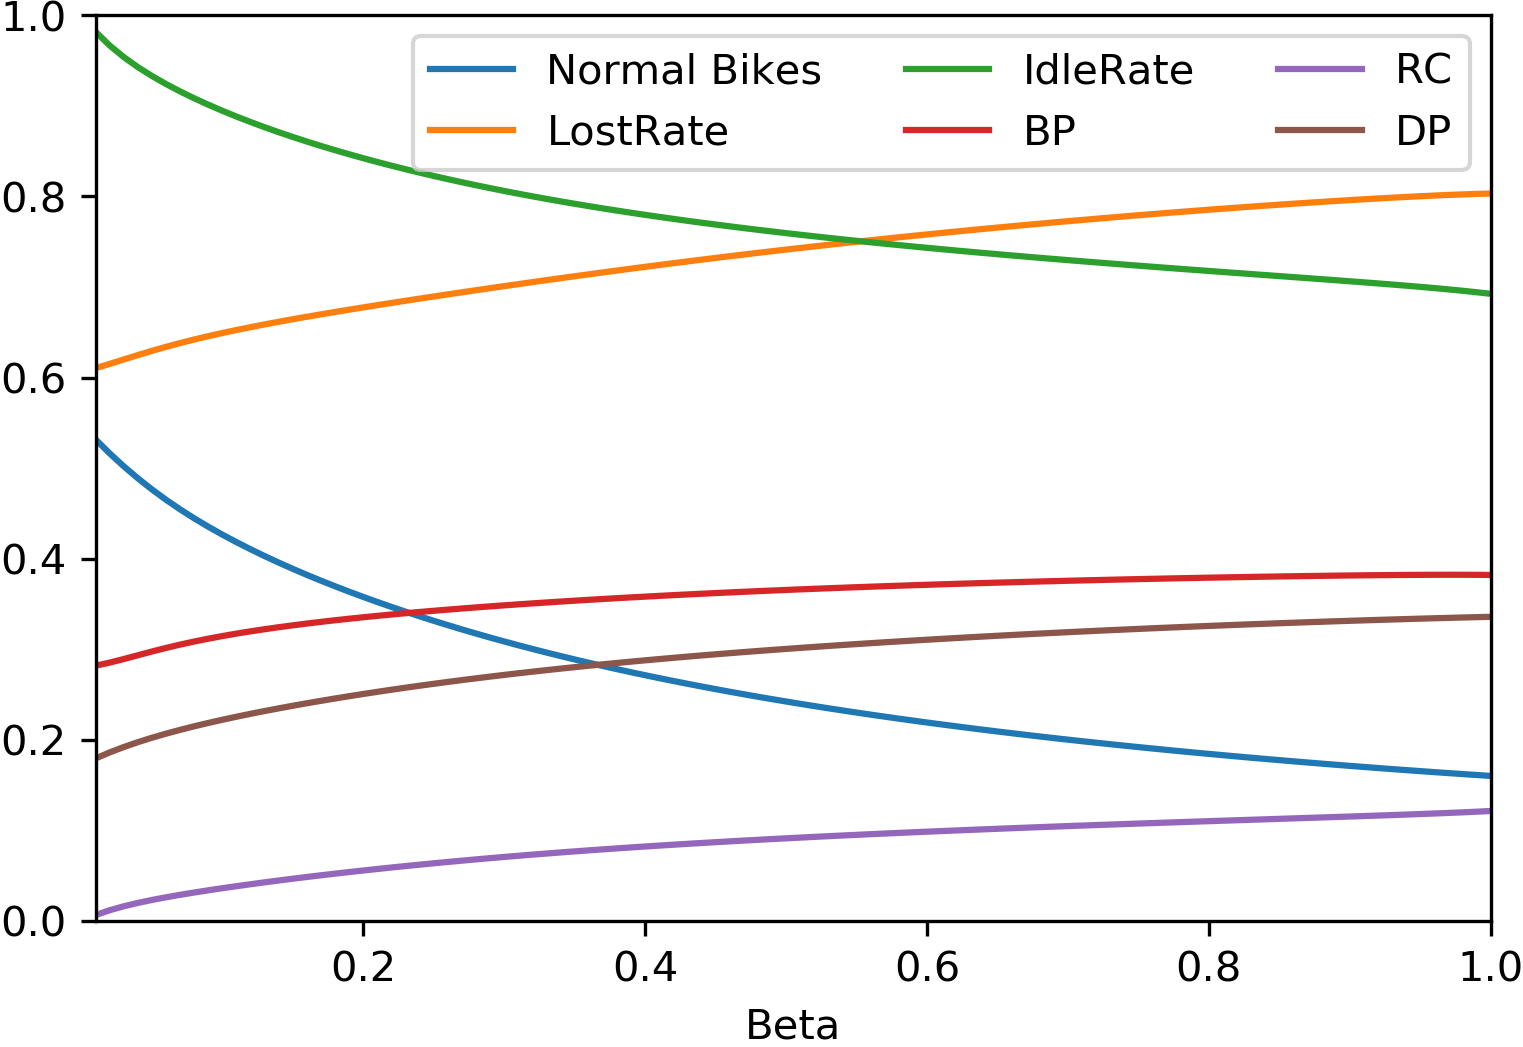
\includegraphics[scale=0.6]{Graph/perfBeta.png}
%     \caption{损坏概率与系统参数变化关系}
%     \label{fig:betaRate}
% \end{figure}
% 随着损坏率的升高系统中好车的比例逐渐下降,顾客的损失比例也会逐渐提高;处在回收、维修和投放过程中的坏车比例升高,维修服务台处在空闲状态的比例逐渐下降。这些现象与常识一致。系统中好车数量下降时,不管系统有怎样的维修能力,在相同的调度安排下,所能服务的顾客数将会减少。同时坏车的数量会增多,处于运维作业过程中的单车比例也会升高。
% 之后,基于给定其他参数的默认值后,进行不同损坏率下系统状态的计算。随着损坏率升高根据观察选取了0.3作为默认值。


% \subsection{实验结果}
% 通过进行数值实验,我们研究共享单车系统中的运维环节对系统整体运行能力的影响。首先我们关注当系统中运维能力有限而要在不同的环节中进行分配的情况。再对各个运维环节的各个参数进行灵敏度分析。在进行数值实验时采用控制变量法。仿真的时间由观察系统进入稳定的时间认为进行确定。

% \subsubsection{运维能力总量有限情况}
% 在实际运营中回收和投放过程是由人工使用运载车搬运完成的。这些人力、车力等通常可以在两项职能中随意切换。因此存在分配的问题。通过在本模型中固定运输速率总和,而变动其中一个,研究系统指标。如图\ref{fig:fixsum}所示。发现当二者相差很大时系统的表现较差。而其余时候表现差异不大。此时提升可分配的总能力,也就是本模型中的二者之和,才可以改善系统表现。但这一改善也存在边际效应递减。同时,提升维修能力也可以一定程度上改善系统的表现。
% $\overline{B}$和$\overline{D}$对系统的影响是相似的。稳态计算和仿真都显示当$\overline{B}$和$\overline{D}$相近时,系统中好车的比例较高。他们对系统性能指标的影响是非单调的,在仿真的结果中可以观察到,系统的表现最初随着批量的升高有所改善,到达某一峰值后开始下降。因此在实践中需要结合经验确定合理的回收批量。
% %\newgeometry{left=0.1cm,right=0.1cm, top=0.1cm, bottom=0.1cm}
% \begin{figure}[H]
%     \centering
%     \subfigure[回收与投放速度总和为定值,变动总和]{
%     \begin{minipage}[t]{0.5\textwidth}
%     \centering
%     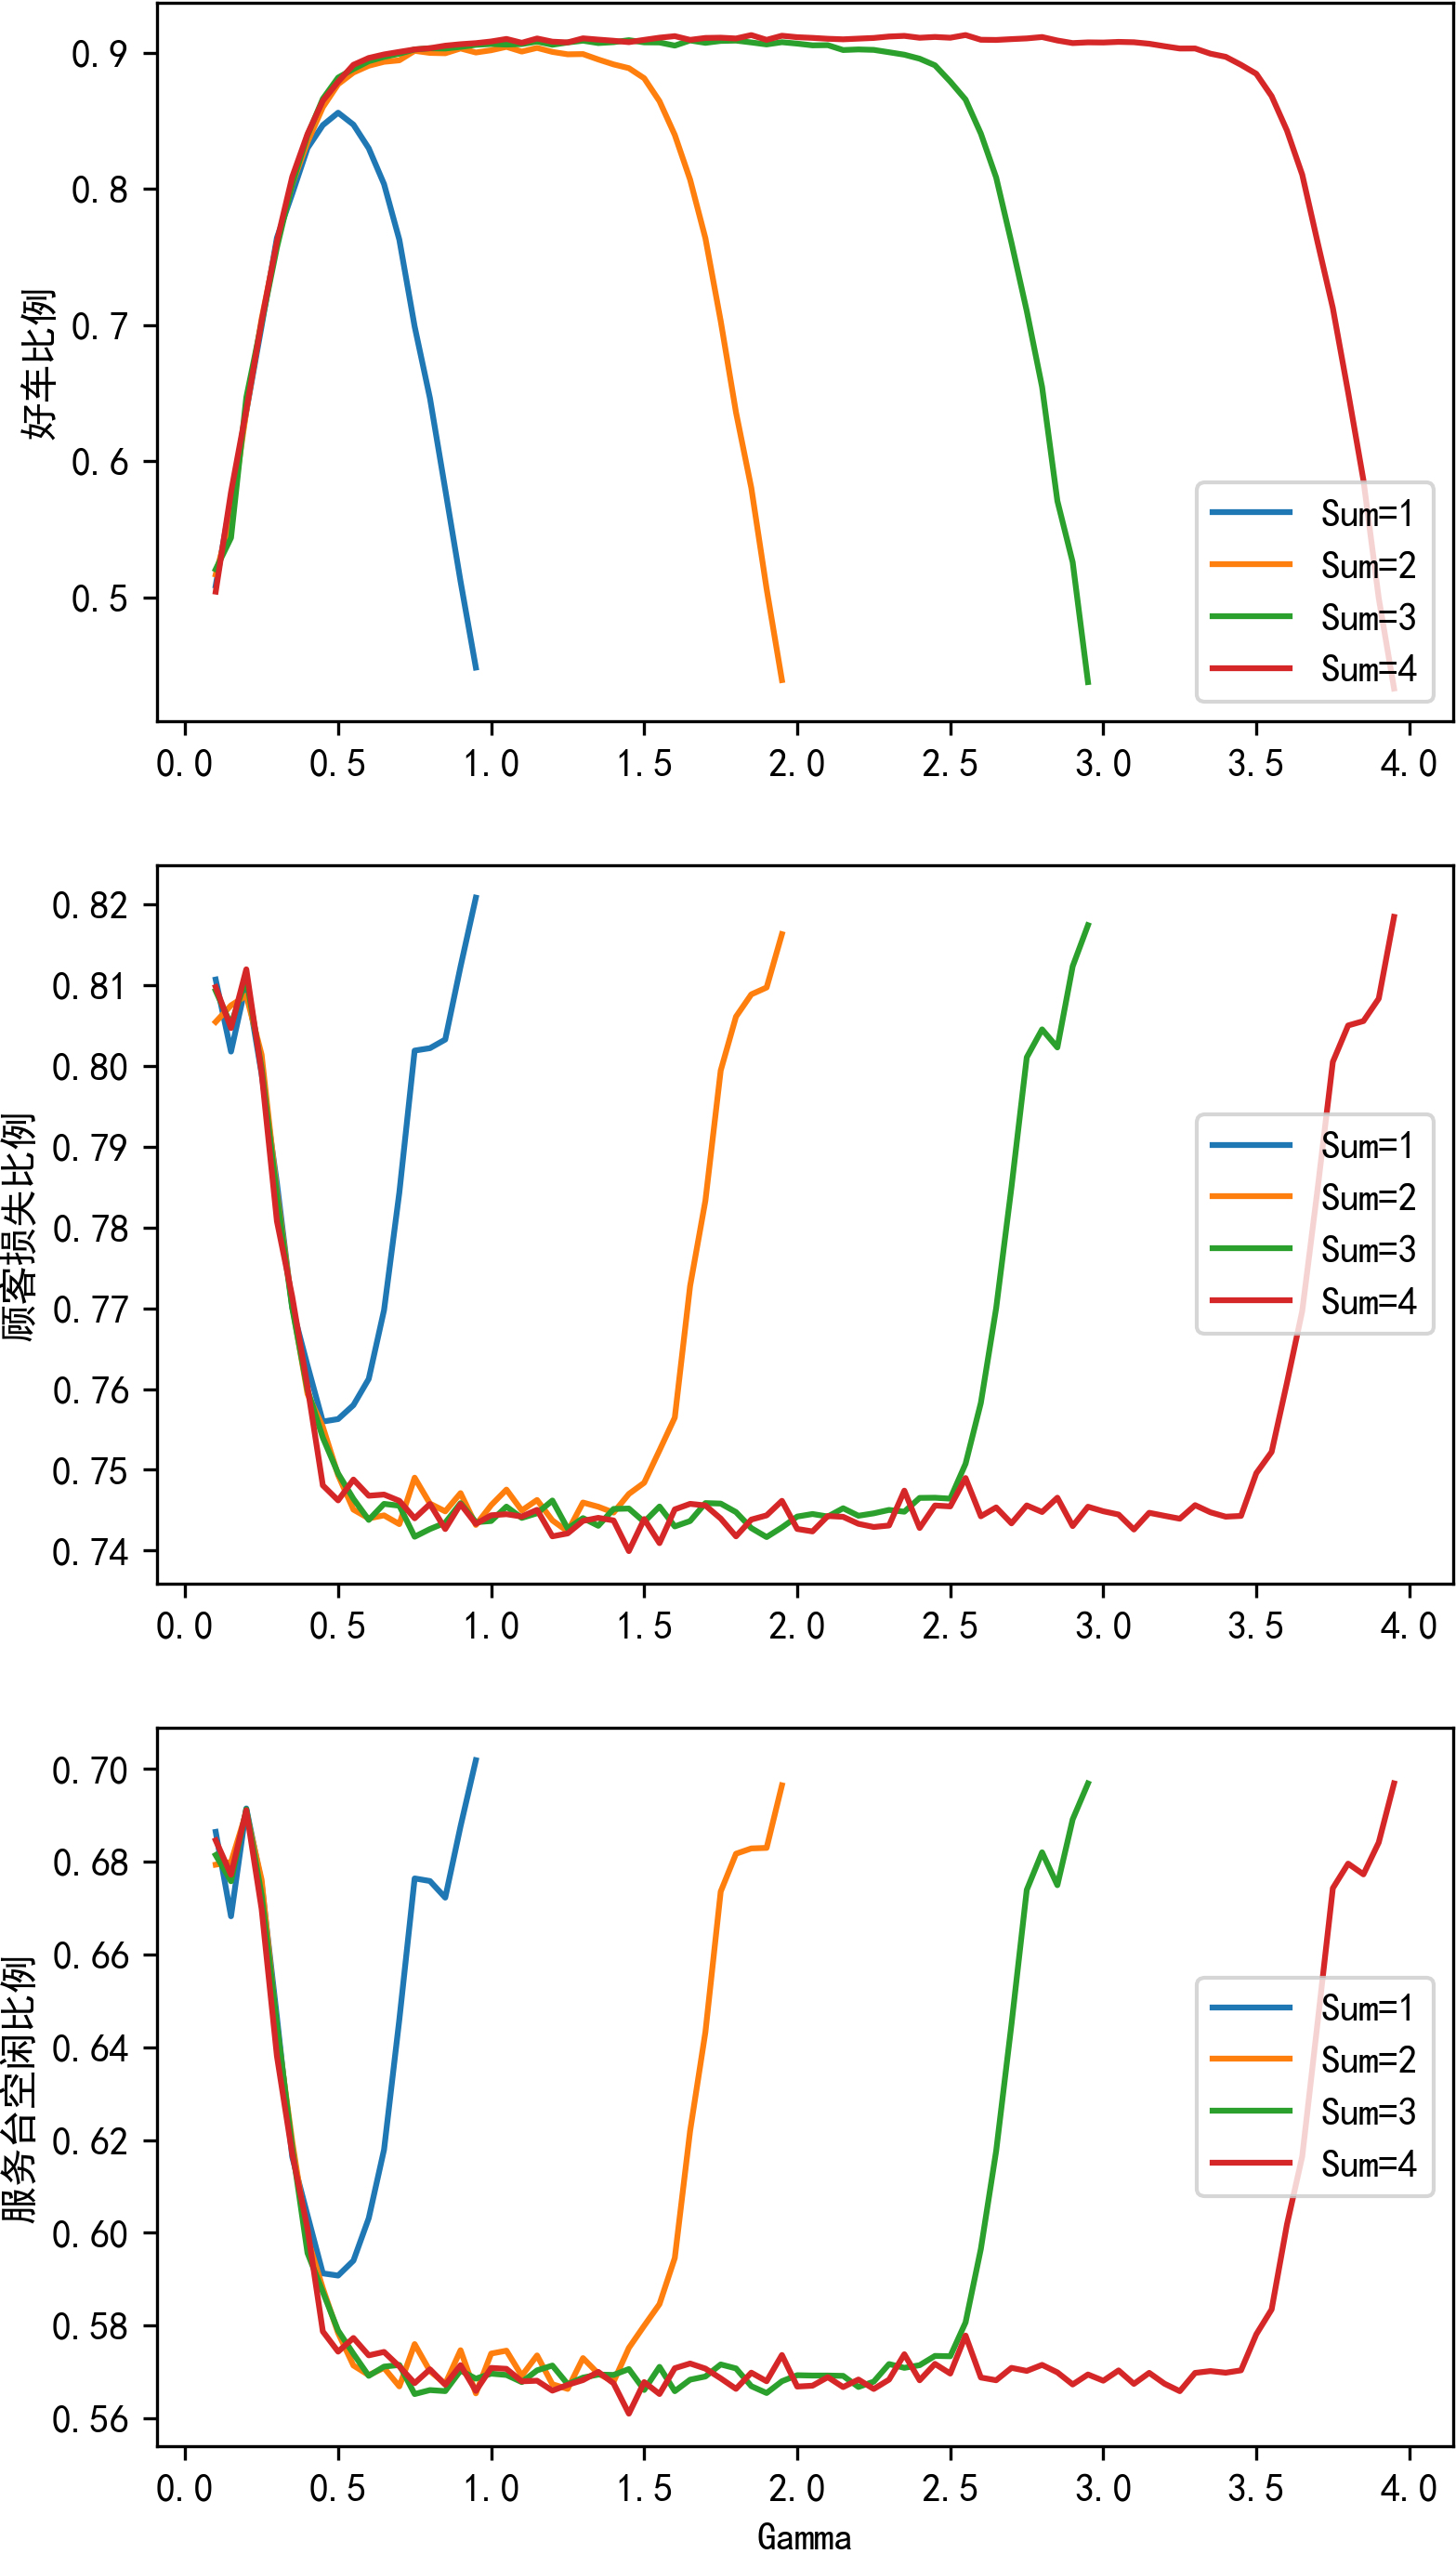
\includegraphics[width=2.4in]{Graph/perf/perfA10M50DeltaGammaSumVaryMu.png}
%     %\caption{fig2}
%     \end{minipage}%
%     }%
%     \centering
%     \subfigure[回收与投放速度总和为定值,变动维修速率]{
%     \begin{minipage}[t]{0.5\textwidth}
%     \centering
%     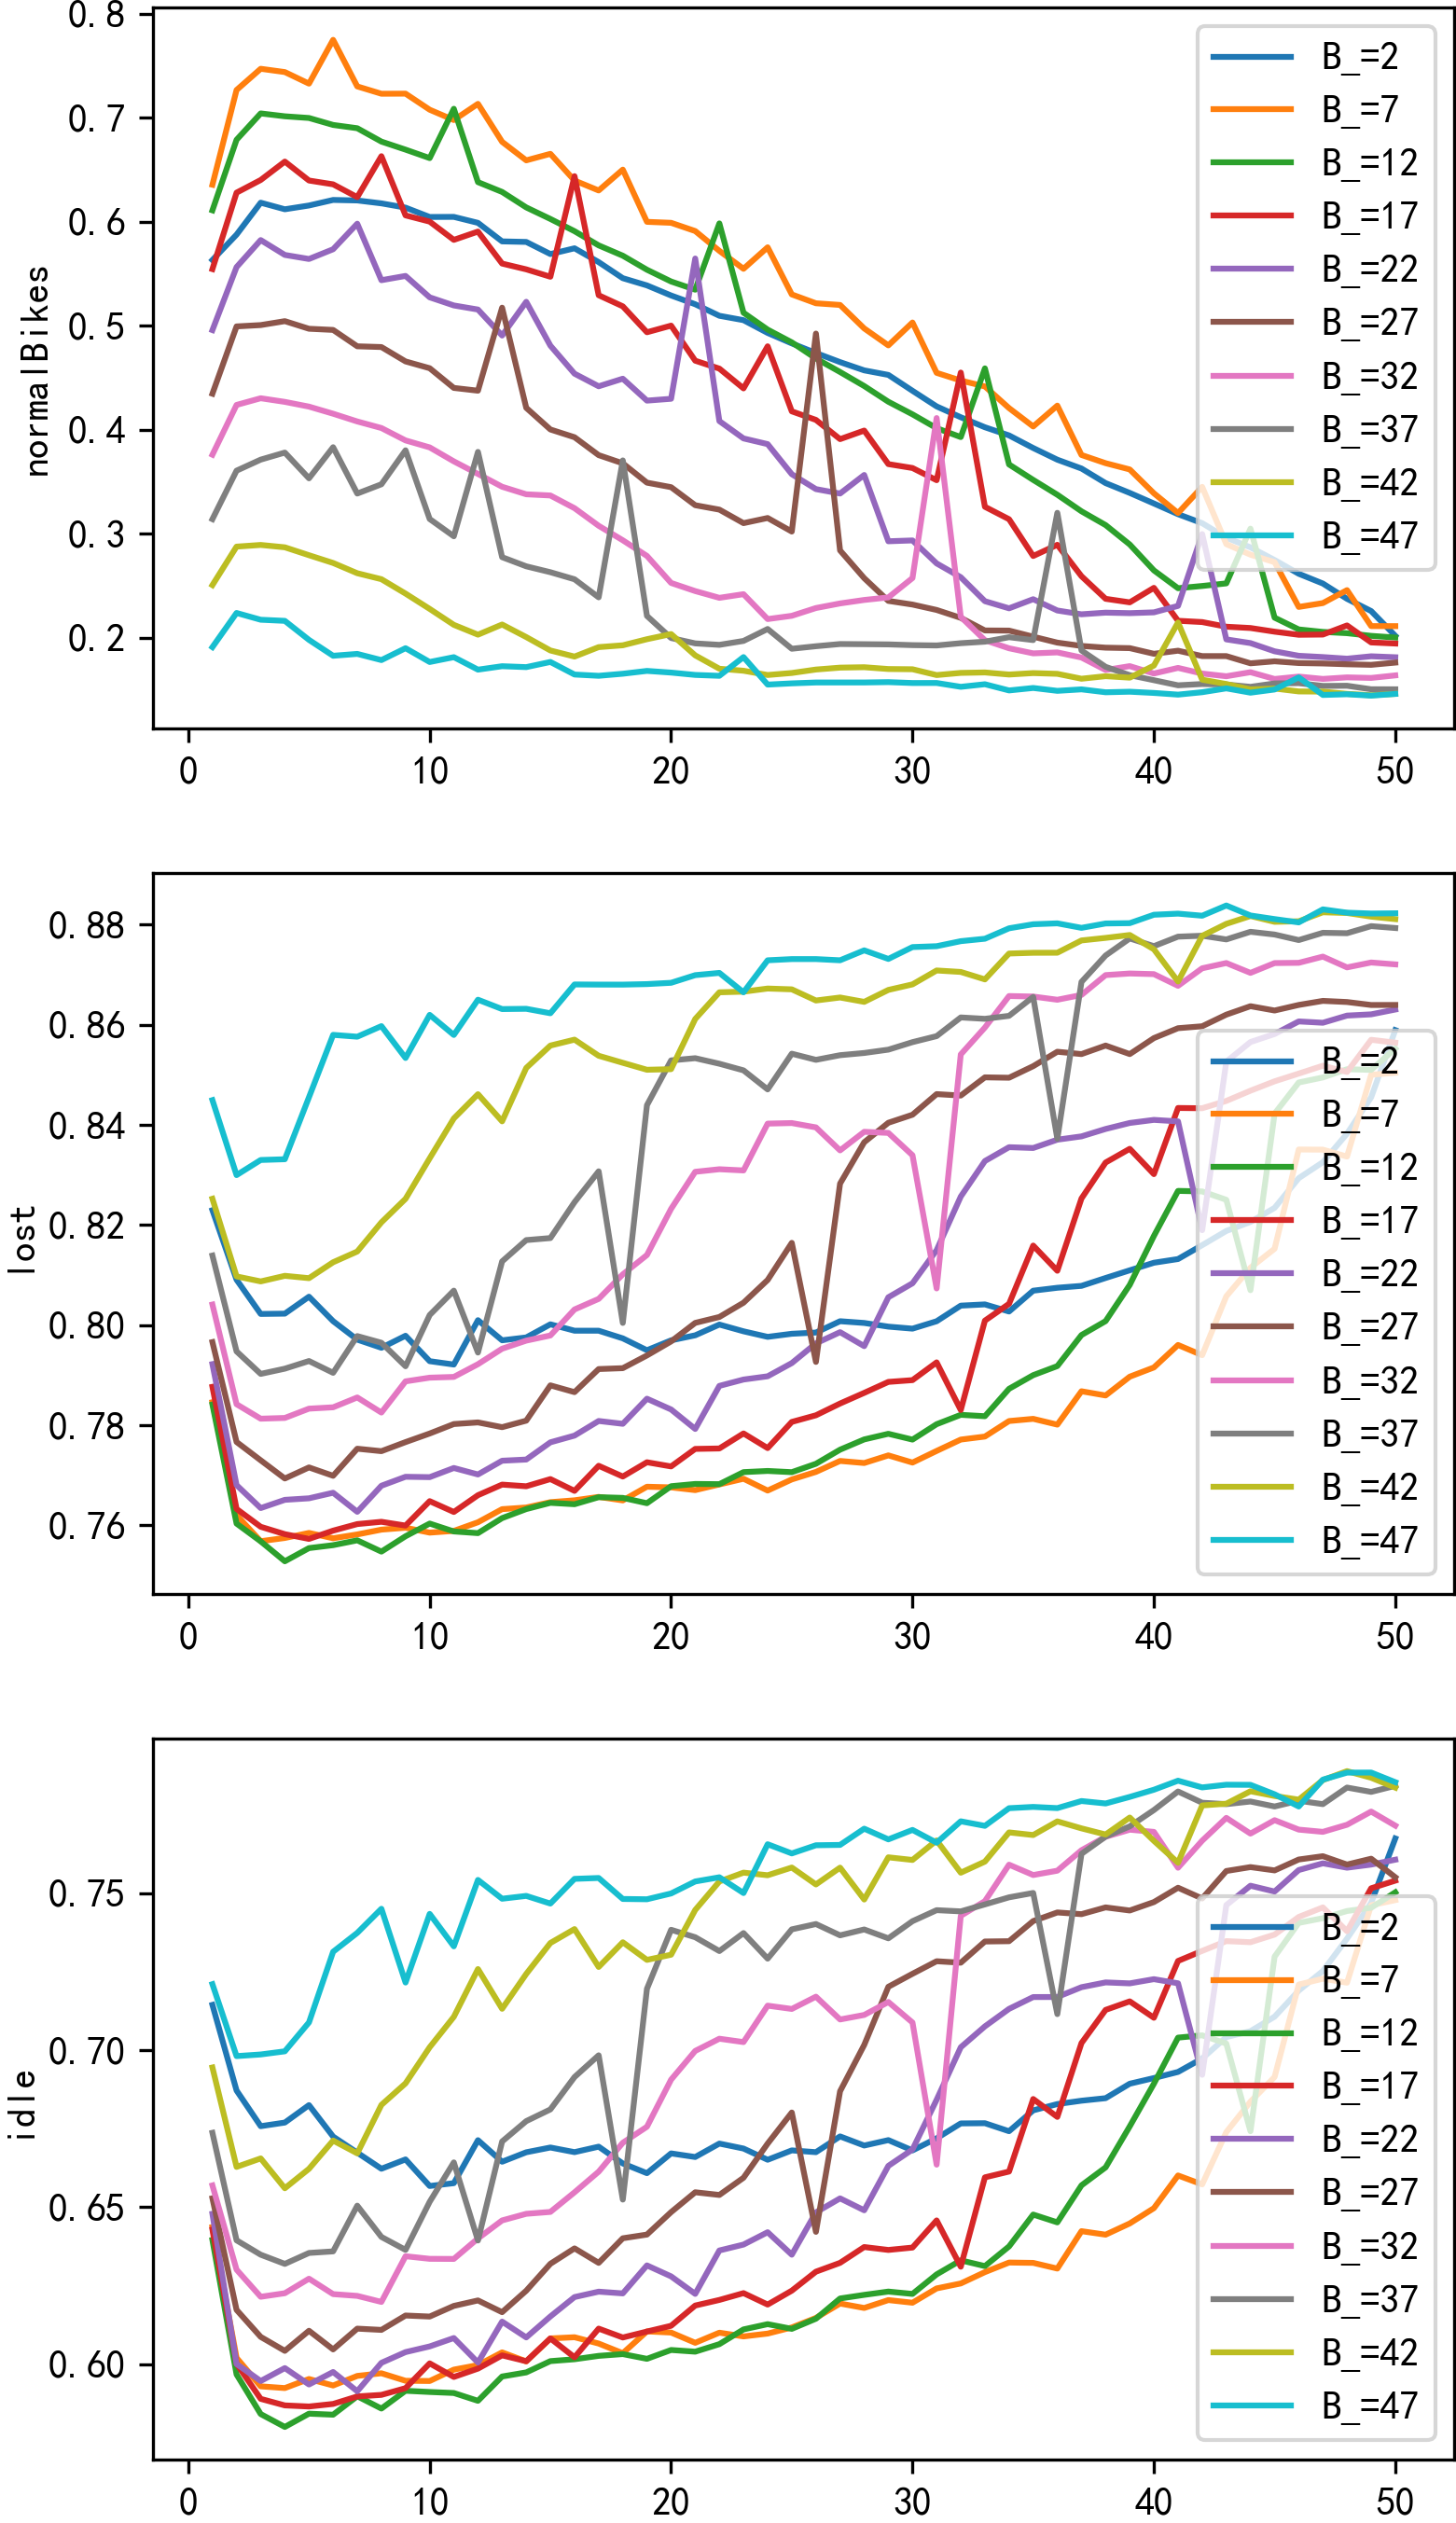
\includegraphics[width=2.3in]{Graph/perf/perfA10M50B_-D_.png}
%     %\caption{fig1}
%     \end{minipage}%
%     }%xs
%     \caption{运维能力总量有限情况}
%     \label{fig:fixsum}
% \end{figure}
% %\restoregeometry

% % \begin{figure}[htbp]

% %     \centering
    
% %     \subfloat[回收与投放速度总和为定值,变动总和]{
    
% %     \label{fig:improved_subfig_a}
    
% %     \begin{minipage}[t]{0.3\textwidth}
    
% %     \centering
    
% %     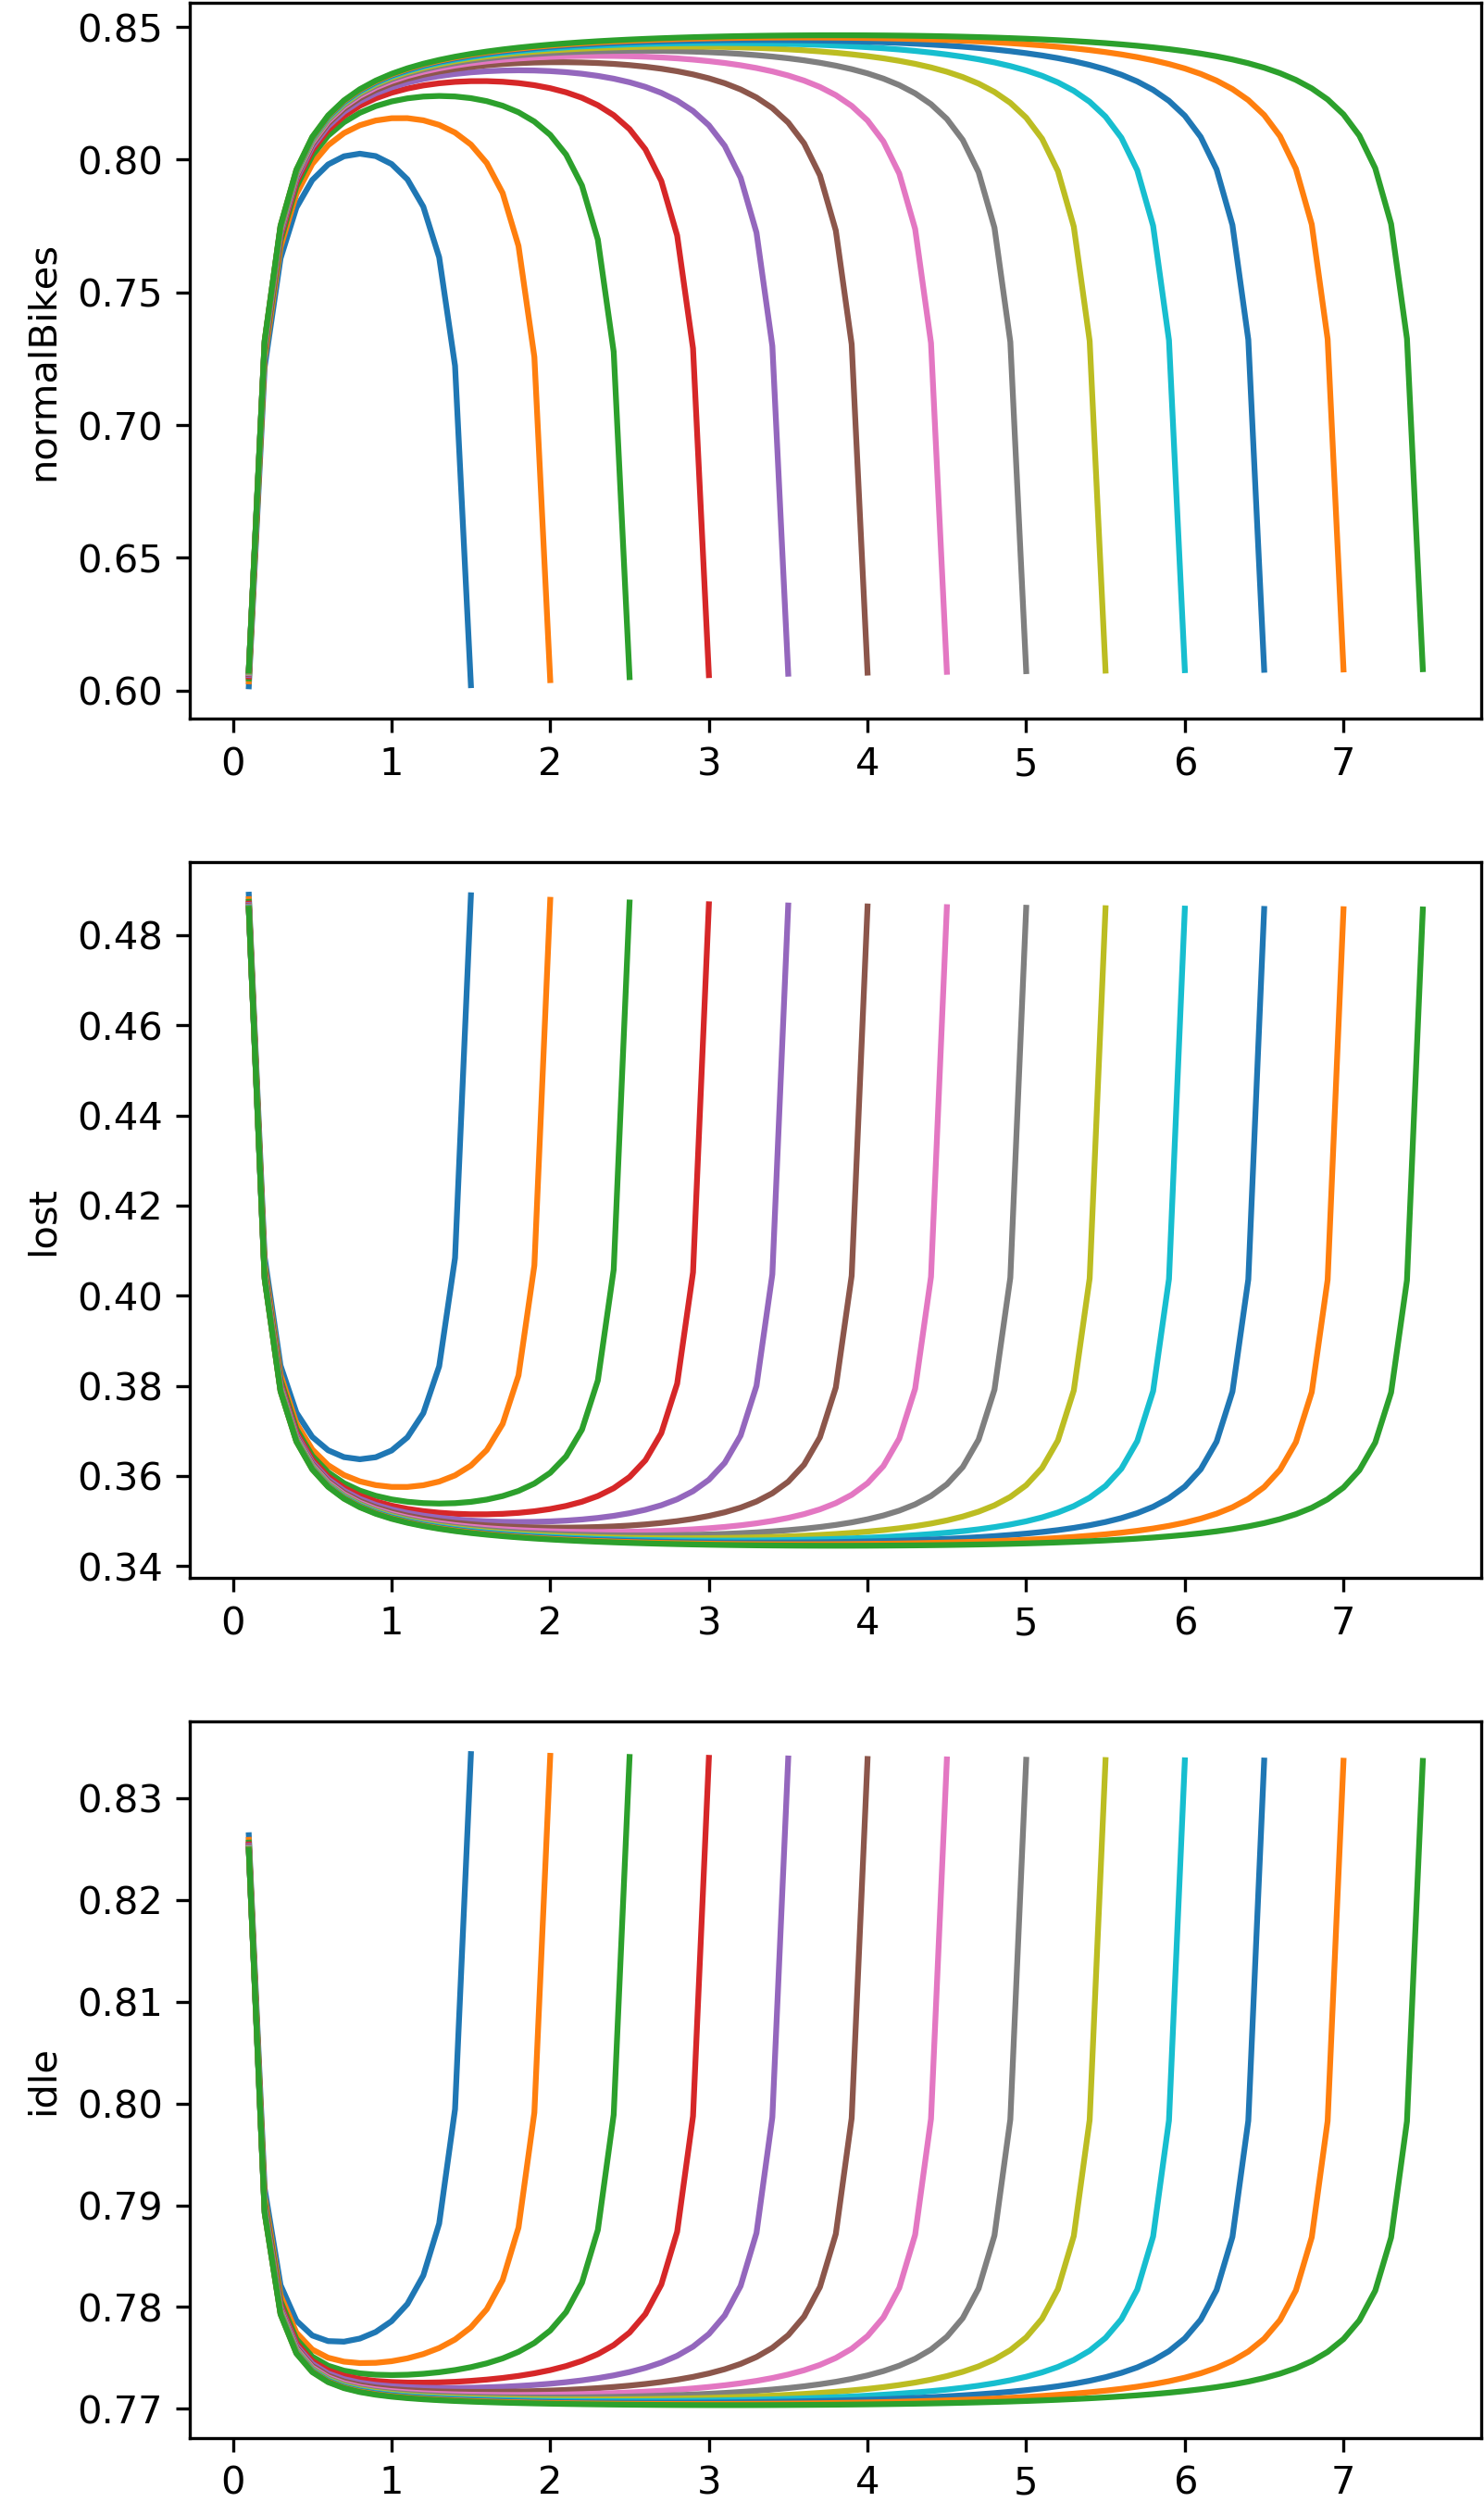
\includegraphics[width=2.4in]{Graph/perf/perfGamma+Delta0-Sum0-8lines.png}
    
% %     \end{minipage}
    
% %     }
    
% %     \subfloat[回收与投放速度总和为定值,变动维修速率]{
    
% %     \label{fig:improved_subfig_b}
    
% %     \begin{minipage}[t]{0.3\textwidth}
    
% %     \centering
    
% %     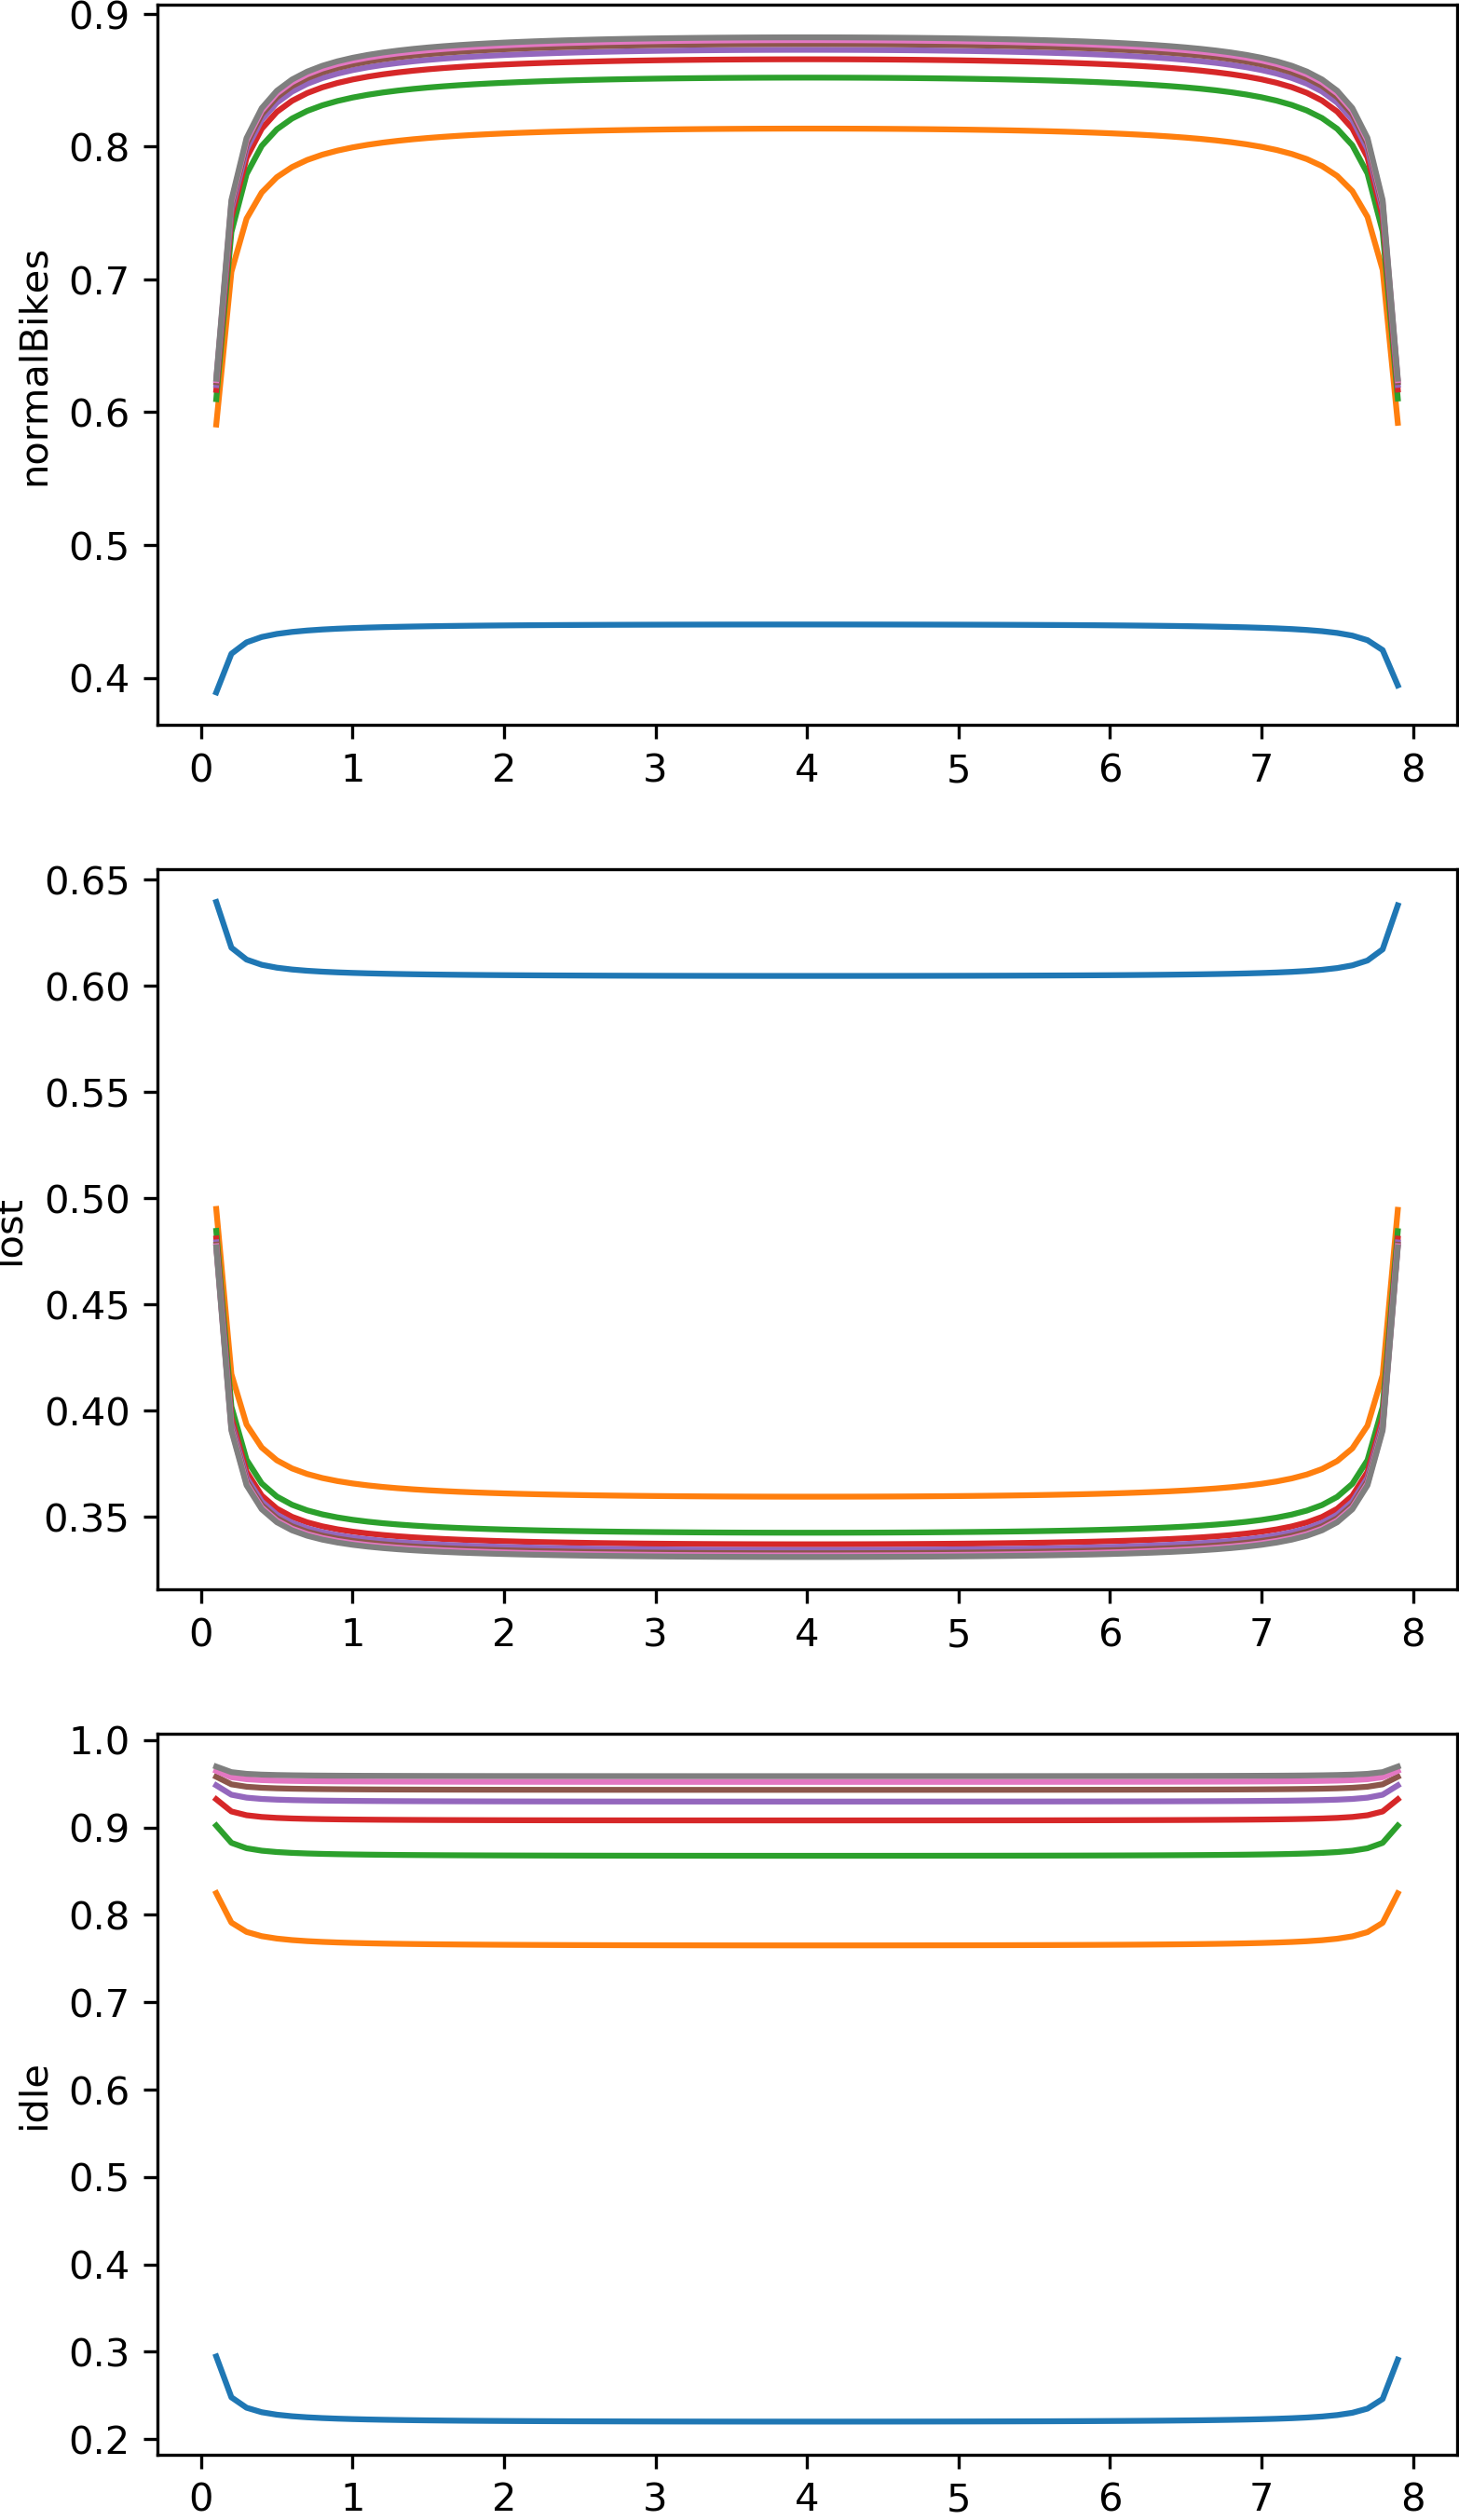
\includegraphics[width=2.3in]{Graph/perf/perfGamma+Delta0-8Mu0-4-8lines.png}
    
% %     \end{minipage}
    
% %     }
    
% %     \caption{运维能力总量有限情况}
% %     \label{fig:fixsum}
    
% %     \end{figure}

% \subsubsection{灵敏度分析}
% 本部分分析某服务环节参数变化对系统运行状态的影响。
% 改善每个环节都可以提升系统,但是有瓶颈。边际效应递减。回收和投放的效果接近。
% 单独提升回收、维修和投放速率能够增大系统中好车的比例,减少客户的损失。改善的效果逐渐减弱,直至不再起作用。
% 回收和投放批量与系统中的好车数和顾客损失率呈阶梯函数关系。总体来说这二者的增大,不利于系统的服务能力的提升。但一定程度的改变不影响系统能力,因此在实际场景中可以通过经验,确定合适的运输批量。

% %\newgeometry{left=0.1cm,right=0.1cm, top=0.1cm, bottom=0.1cm}
% \begin{figure}[H]
%     \centering
%     \subfigure[$\overline{B}$-Gamma]{
%     \begin{minipage}[t]{0.5\linewidth}
%     \centering
%     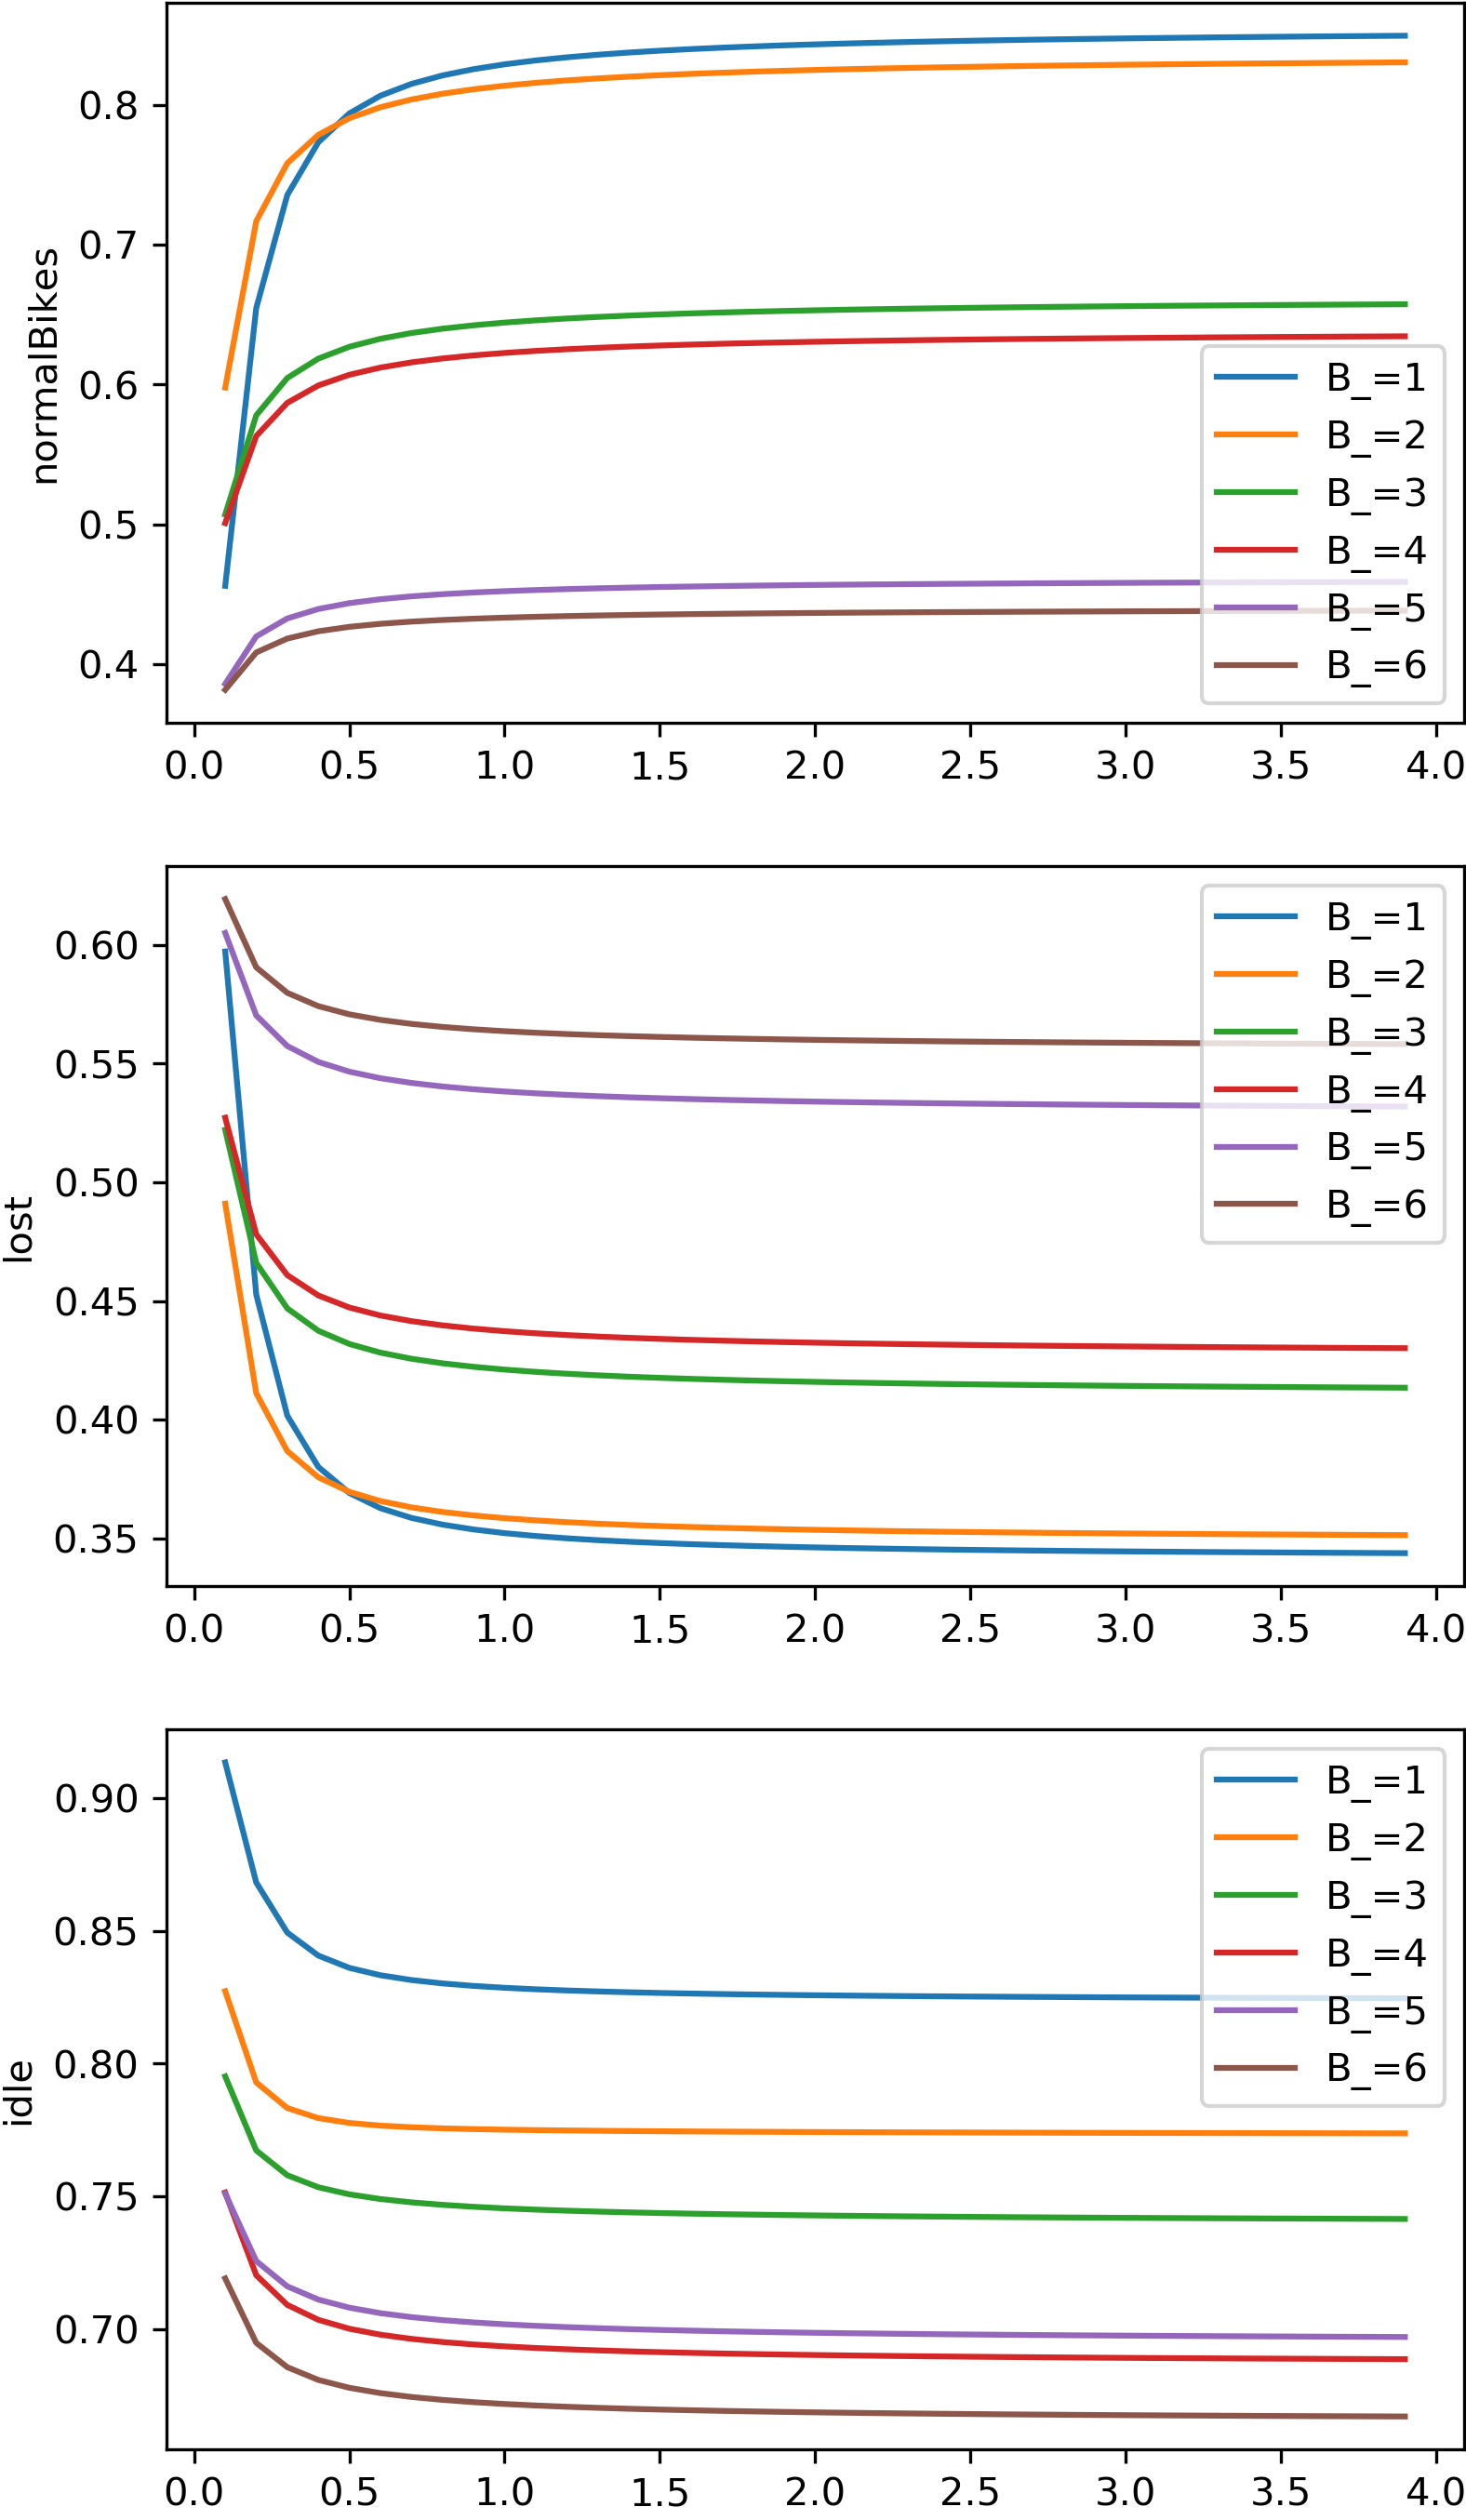
\includegraphics[width=2.25in]{Graph/perf/perfB_1-6Gamma0-4.png}
%     %\caption{fig1}
%     \end{minipage}%
%     }%
%     \centering
%     \subfigure[N-Mu]{
%     \begin{minipage}[t]{0.5\linewidth}
%     \centering
%     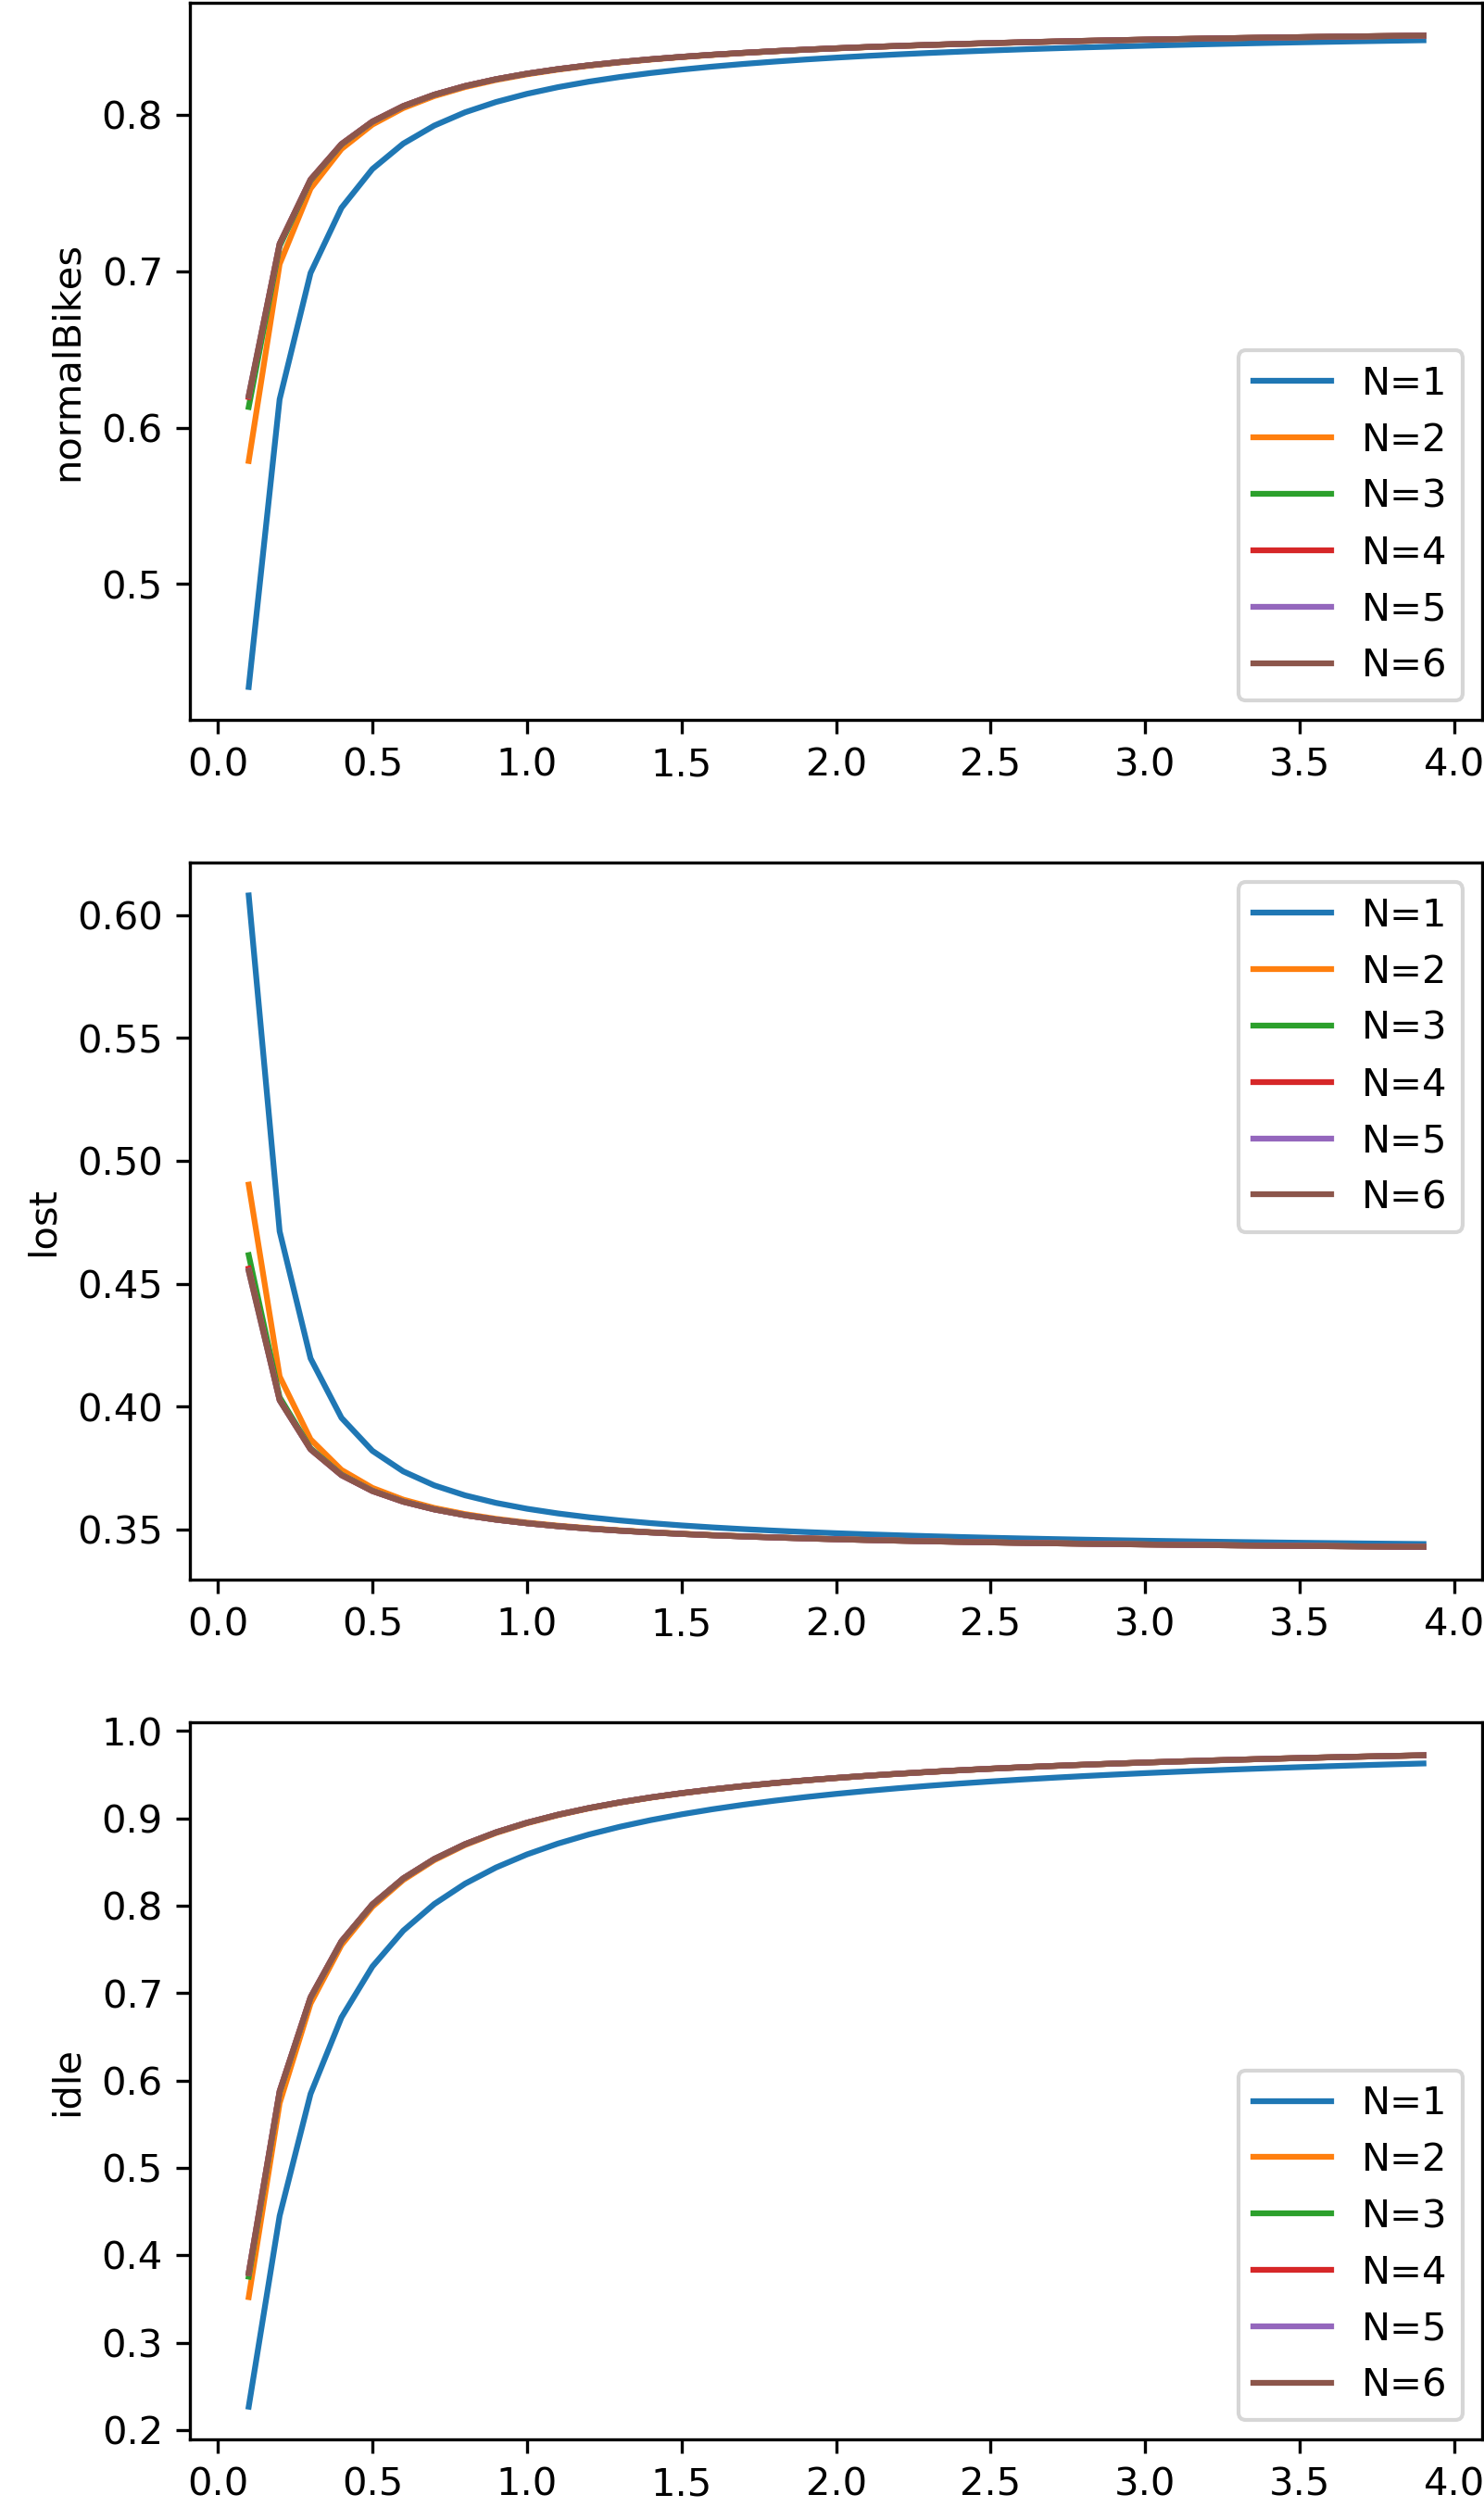
\includegraphics[width=2.3in]{Graph/perf/perfNMu.png}
%     %\caption{fig2}
%     \end{minipage}%
%     }%
% \end{figure}
% %\restoregeometry

% %\newgeometry{left=0.1cm,right=0.1cm, top=0.1cm, bottom=0.1cm}
% \begin{figure}[H]
%     \centering
%     \subfigure[$\overline{D}$-Delta]{
%     \begin{minipage}[t]{0.5\linewidth}
%     \centering
%     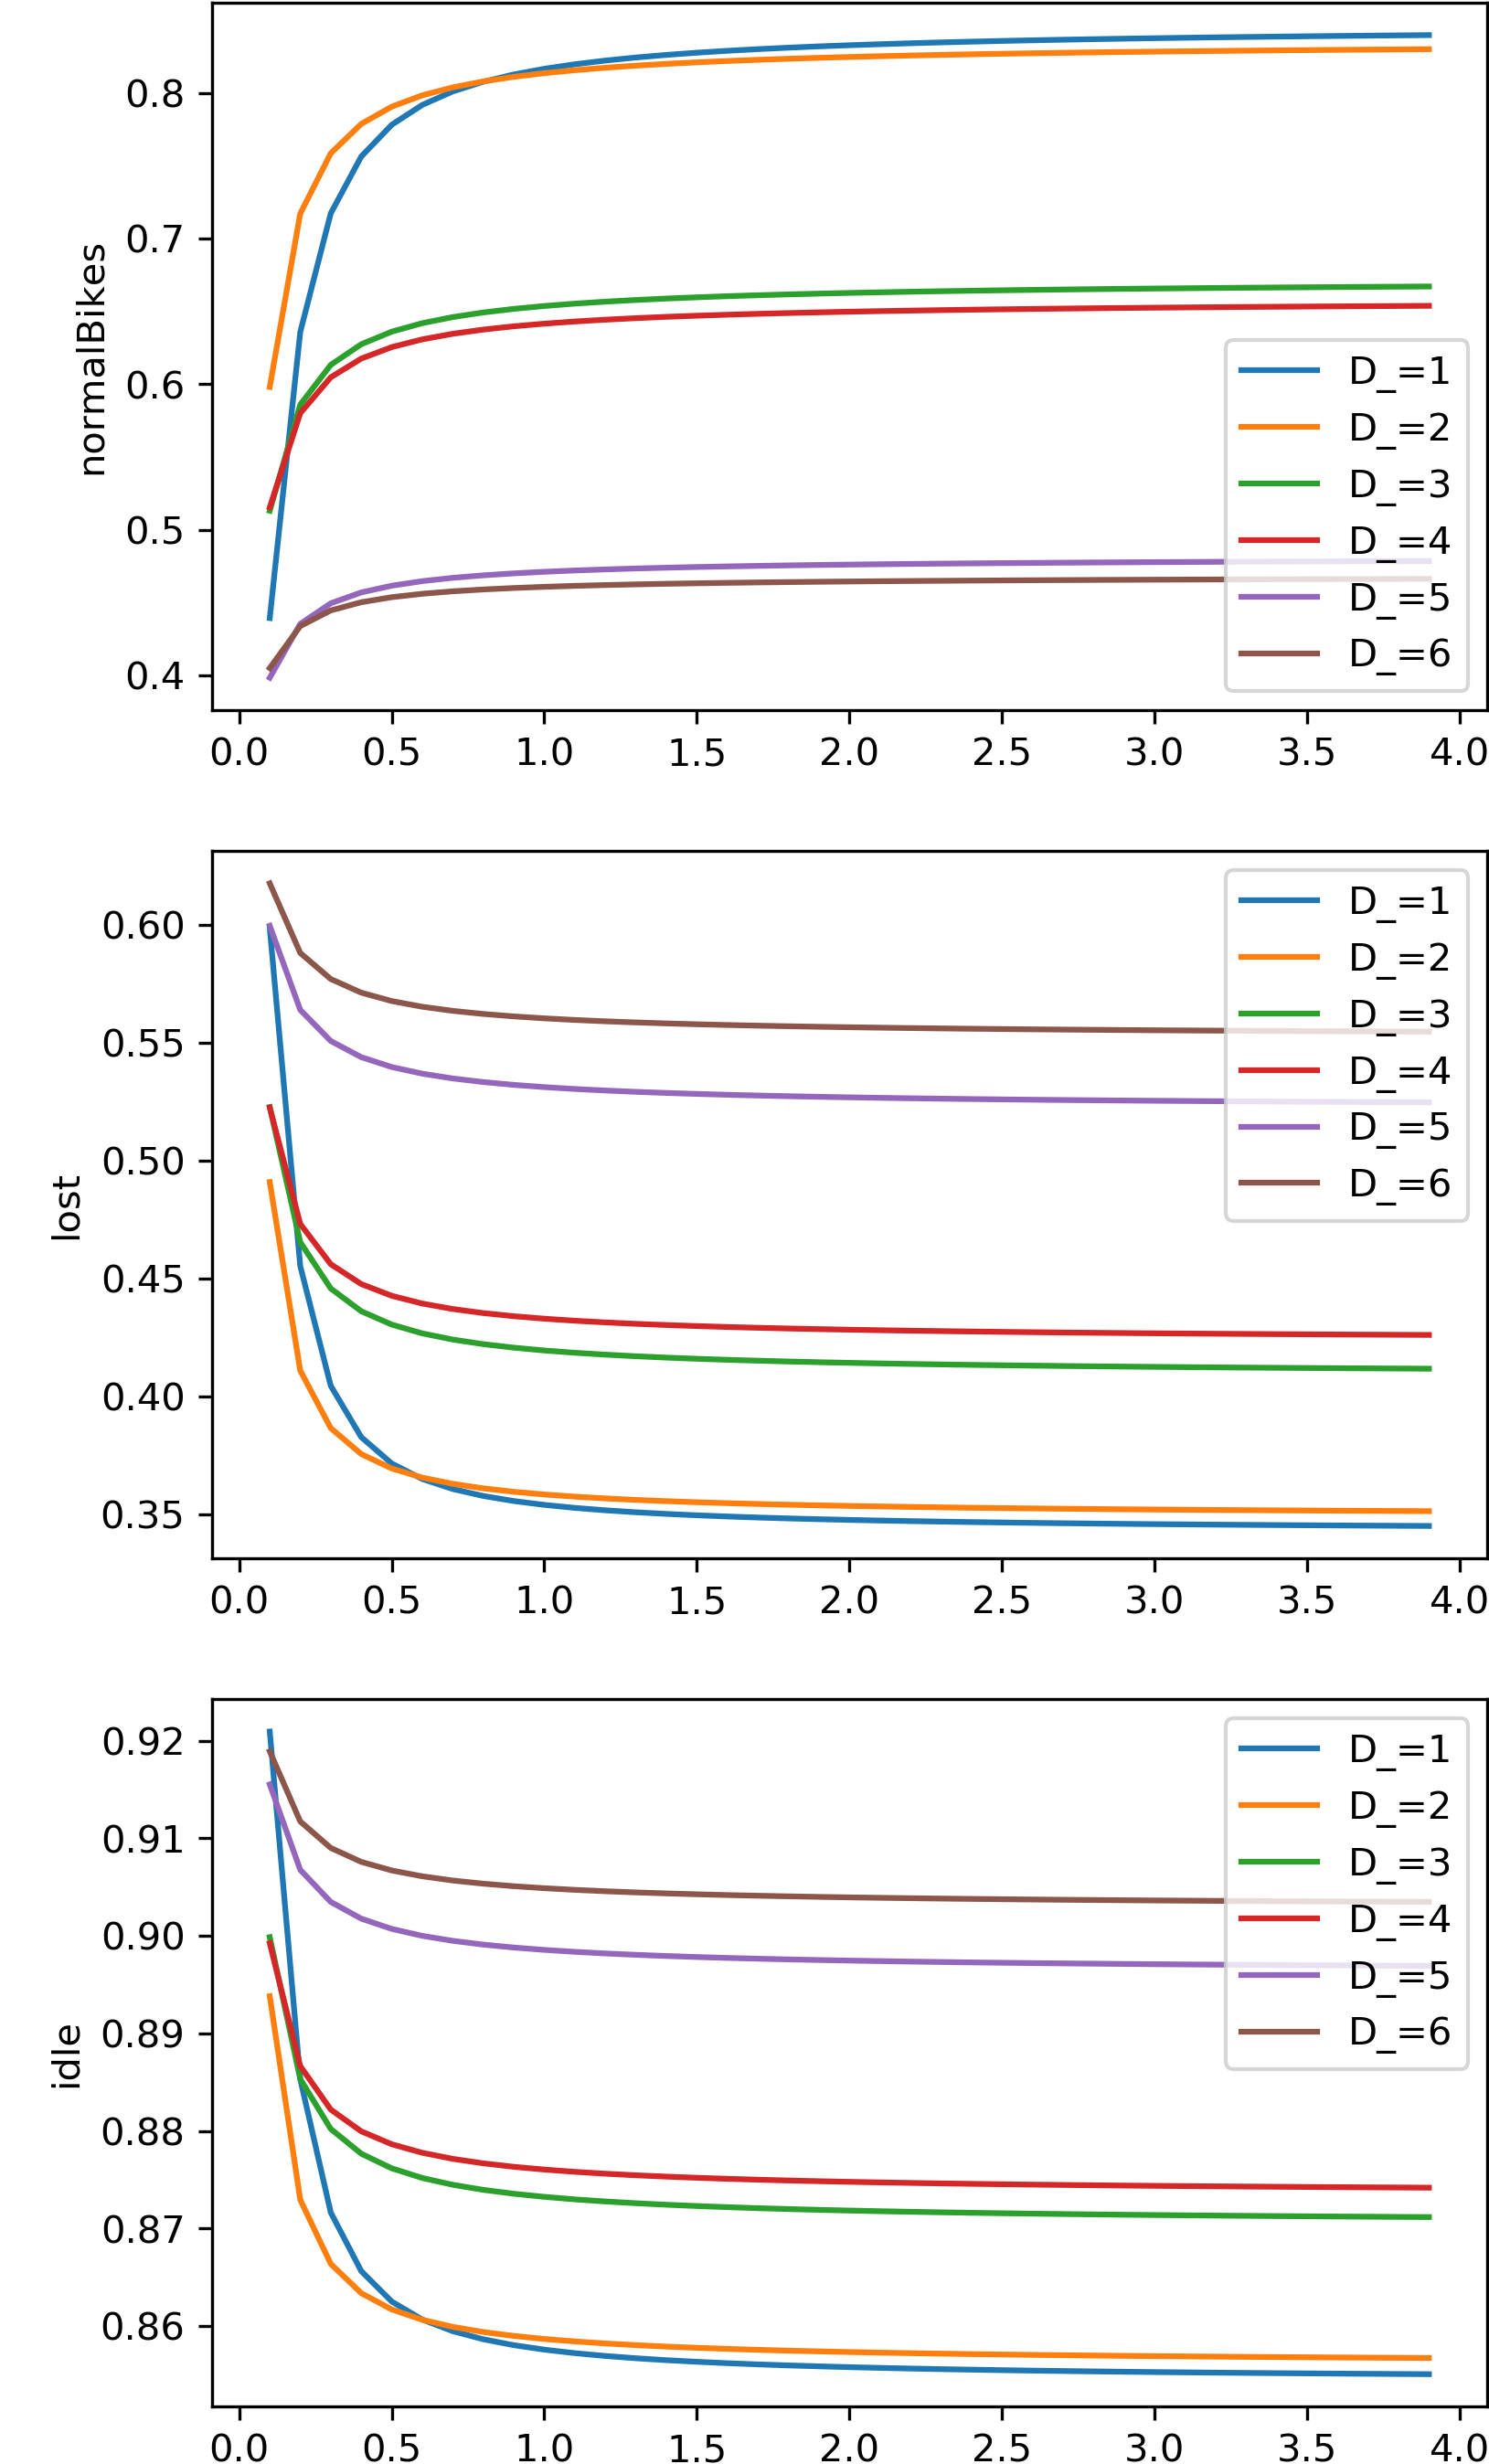
\includegraphics[width=2.4in]{Graph/perf/perfD_Delta.png}
%     %\caption{fig2}
%     \end{minipage}%
%     }%
%     \centering
%     \subfigure[$\overline{B}-\overline{D}$]{
%     \begin{minipage}[t]{0.5\linewidth}
%     \centering
%     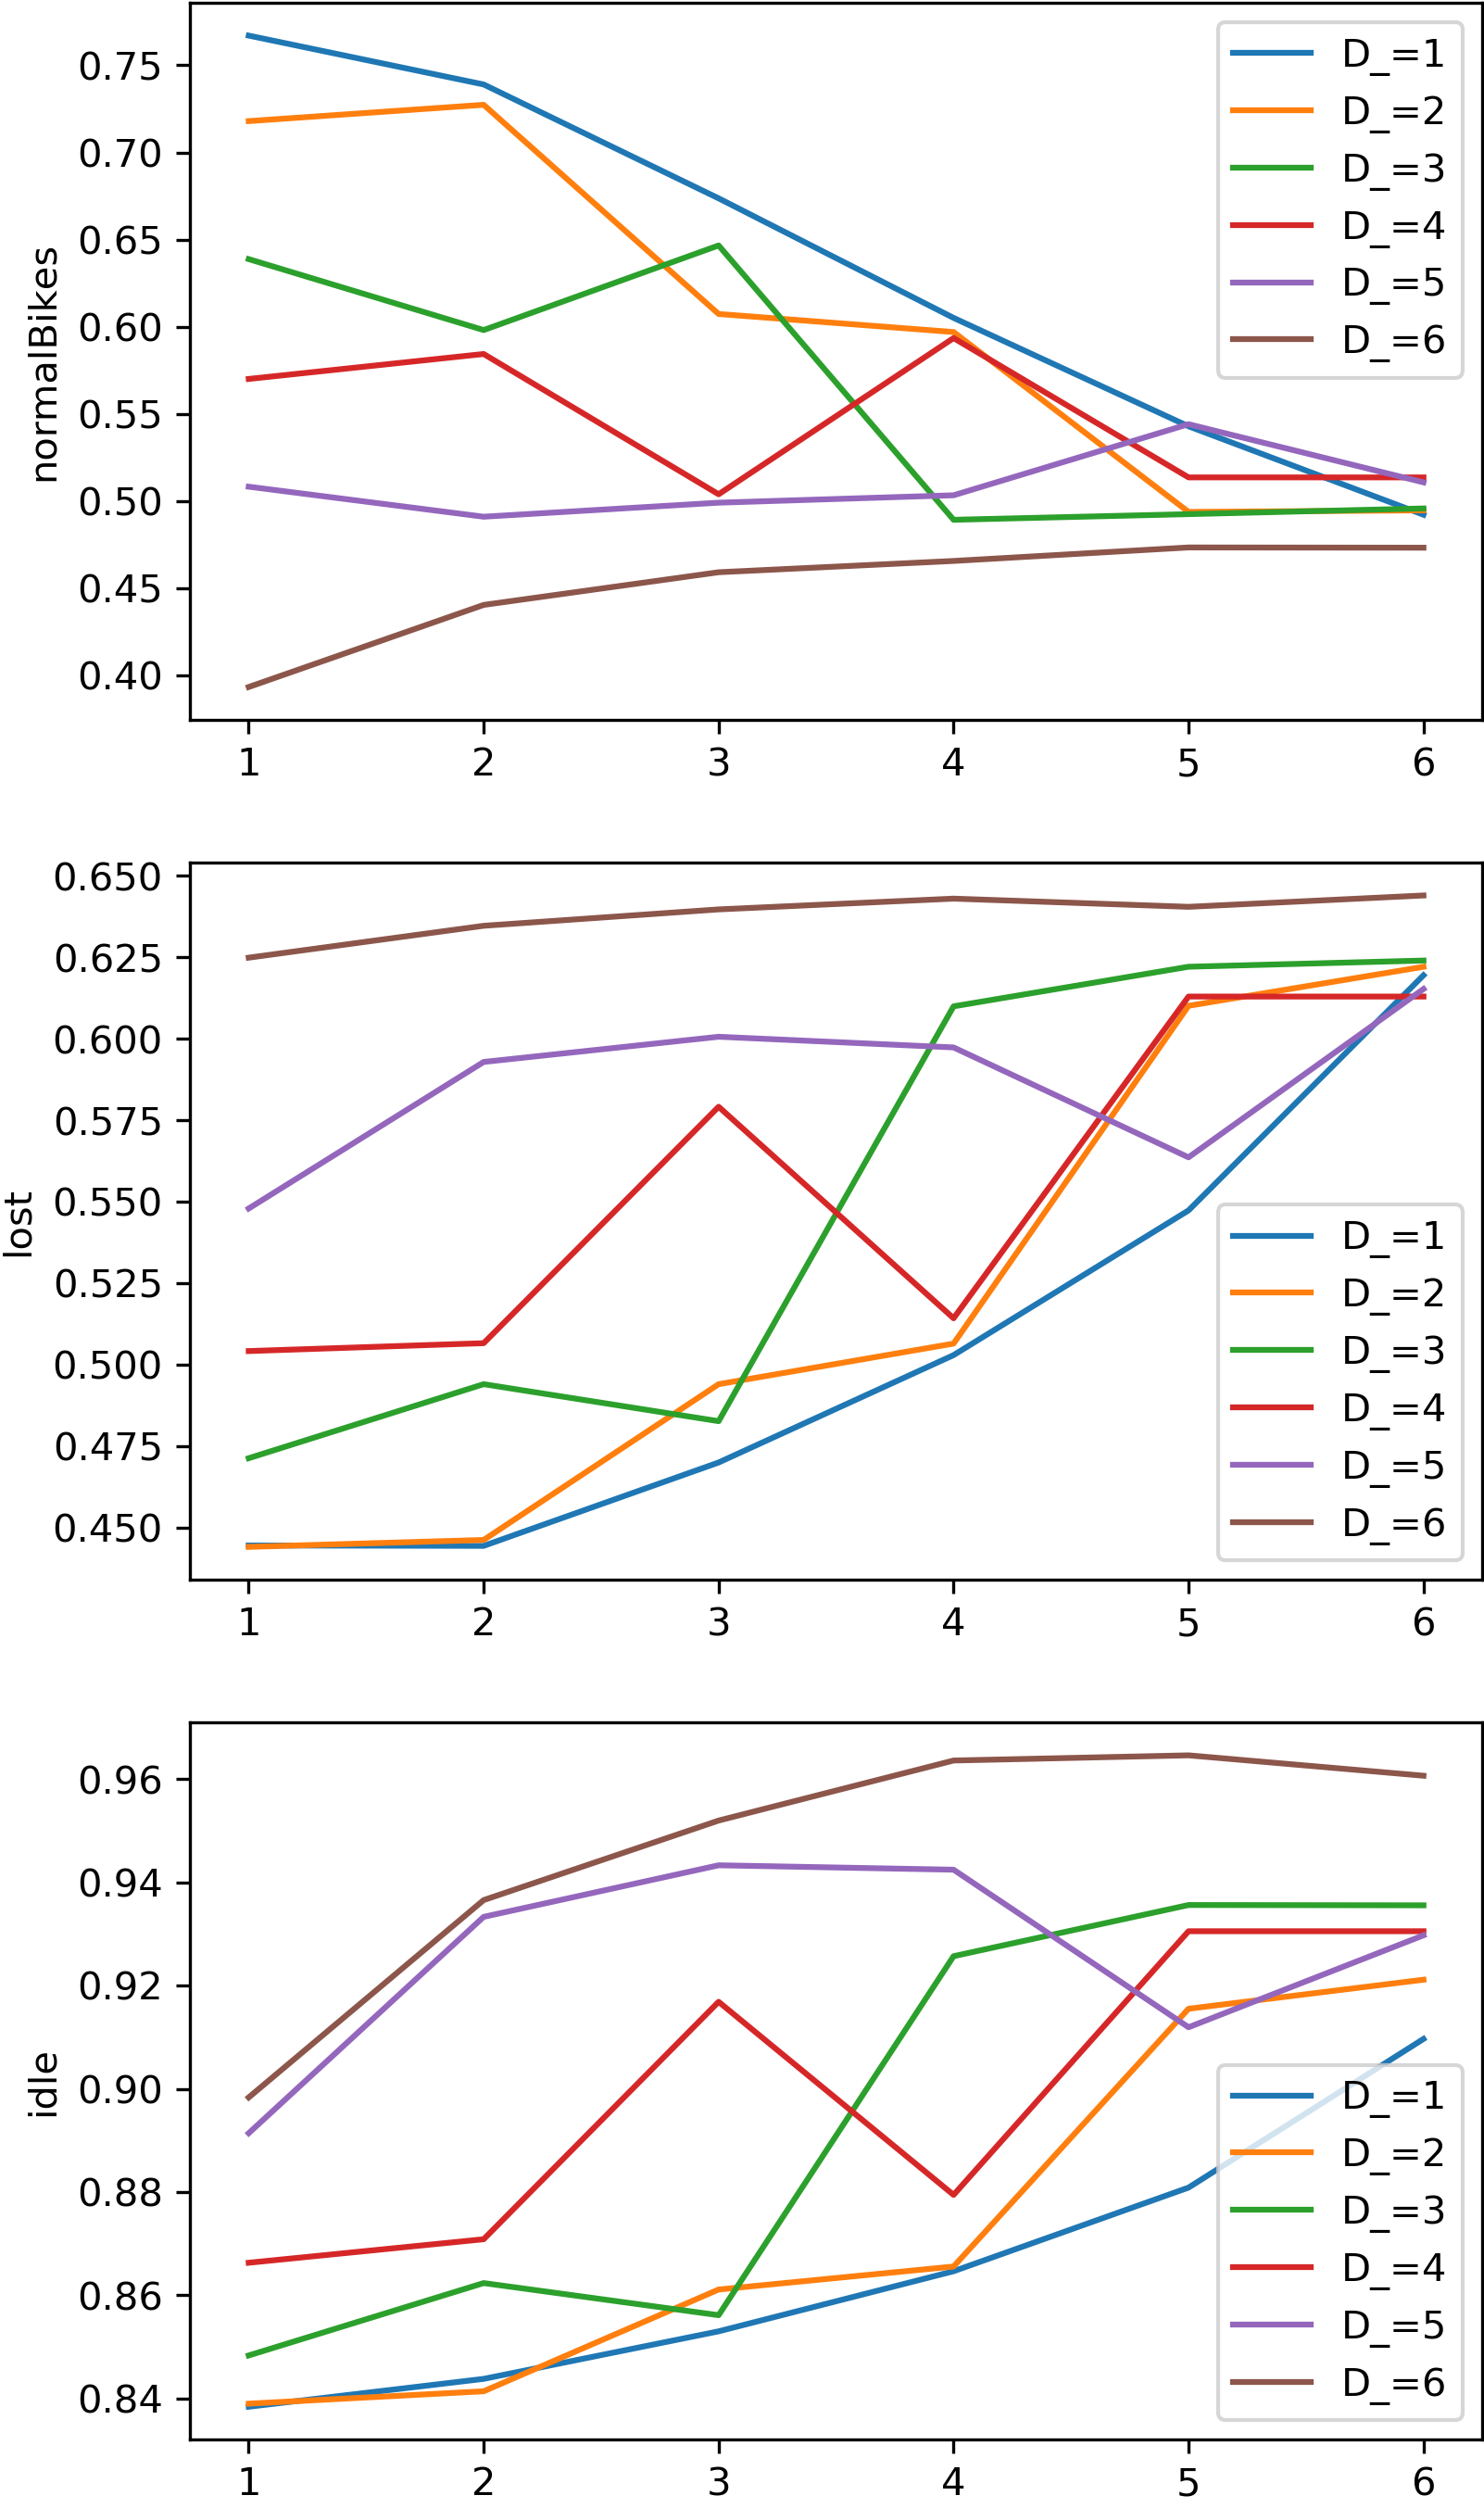
\includegraphics[width=2.3in]{Graph/perf/D_-B_.png}
%     %\caption{fig1}
%     \end{minipage}%
%     }%
%     % \caption{运维能力总量有限情况}
%     % \label{fig:fixsum}
% \end{figure}
%\restoregeometry



% \begin{itemize}
%     \item 损坏率升高,系统中的好车比例降低,顾客损失率普遍升高
%     \item 各个单个参数的效果
%     \item 每个部分的效果
%     \item 系统能力有限,在几个之间平衡时的效果
%     \item 维修速率的提高可以迅速改善系统的服务能力,但是单纯改善维修能力带来的改善是有限的,还会受到其他因素的限制。
%     \item 维修台带来的改善与维修速率类似,只是改善的程度更弱。
%     \item 损坏率的升高或者维修能力的改善,在某些情况下可能并不改善系统中顾客的损失情况
%     \item 对比而言,损坏率对两种模式有着显著不同的影响。在相同维修能力下,分散式的维修情况下系统中的好车数始终多于集中式维修。单独提升维修速度或者维修服务台的数量,维修的所能发挥的改善作用对二者而言是类似的,但是分散式的最大上限会更高。
%     \item 要匹配搬运能力、维修能力、维修台数量和投放能力,一个过高是没有意义的,边际效用递减
%     \item 搬运和投放能力相近时系统的好车比例最高
% \end{itemize}


\section{结论}
通过将共享单车的服务过程和坏车运维过程抽象成排队过程,将共享单车的运维建模成封闭的排队网络,构建了对应的马尔可夫链。通过马尔可夫链存在的长程稳定状态比率进一步计算得到系统的性能指标。最后通过变动系统参数,观察运维能力变化时指标的相应变化。结果显示,提升总的运维能力可以提升系统中的好车比例,降低顾客损失。当运维总能力有限,对共享单车的坏车进行运维时,要尽可能保持回收和投放的速率相一致。在此基础上提升维修能力,可以改善系统状况。但是改善的效果存在边际递减效应。各个环节的能力也存在相同情况。而回收和投放的批量应当尽可能小,以尽快将损坏的车进行维修,修好的车重新投入服务中。在实际中可以结合实际成本等,确定最佳运维安排。

\newpage
\bibliographystyle{plain}
\bibliography{references.bib}

\newpage
\normalsize\textbf{ 附录 }
\begin{figure}[H]
    \centering
    \subfigure[时间长度]{
    \begin{minipage}[t]{0.5\linewidth}
    \centering
    \includegraphics[width=2.4in]{Graph/A10M50系统性能参数-时间40000图.png}
    %\caption{fig2}
    \end{minipage}%
    }%
\end{figure}
\begin{figure}[H]
    \centering
    \subfigure[$\overline{B}-\overline{D}$]{
    \begin{minipage}[t]{0.5\linewidth}
    \centering
    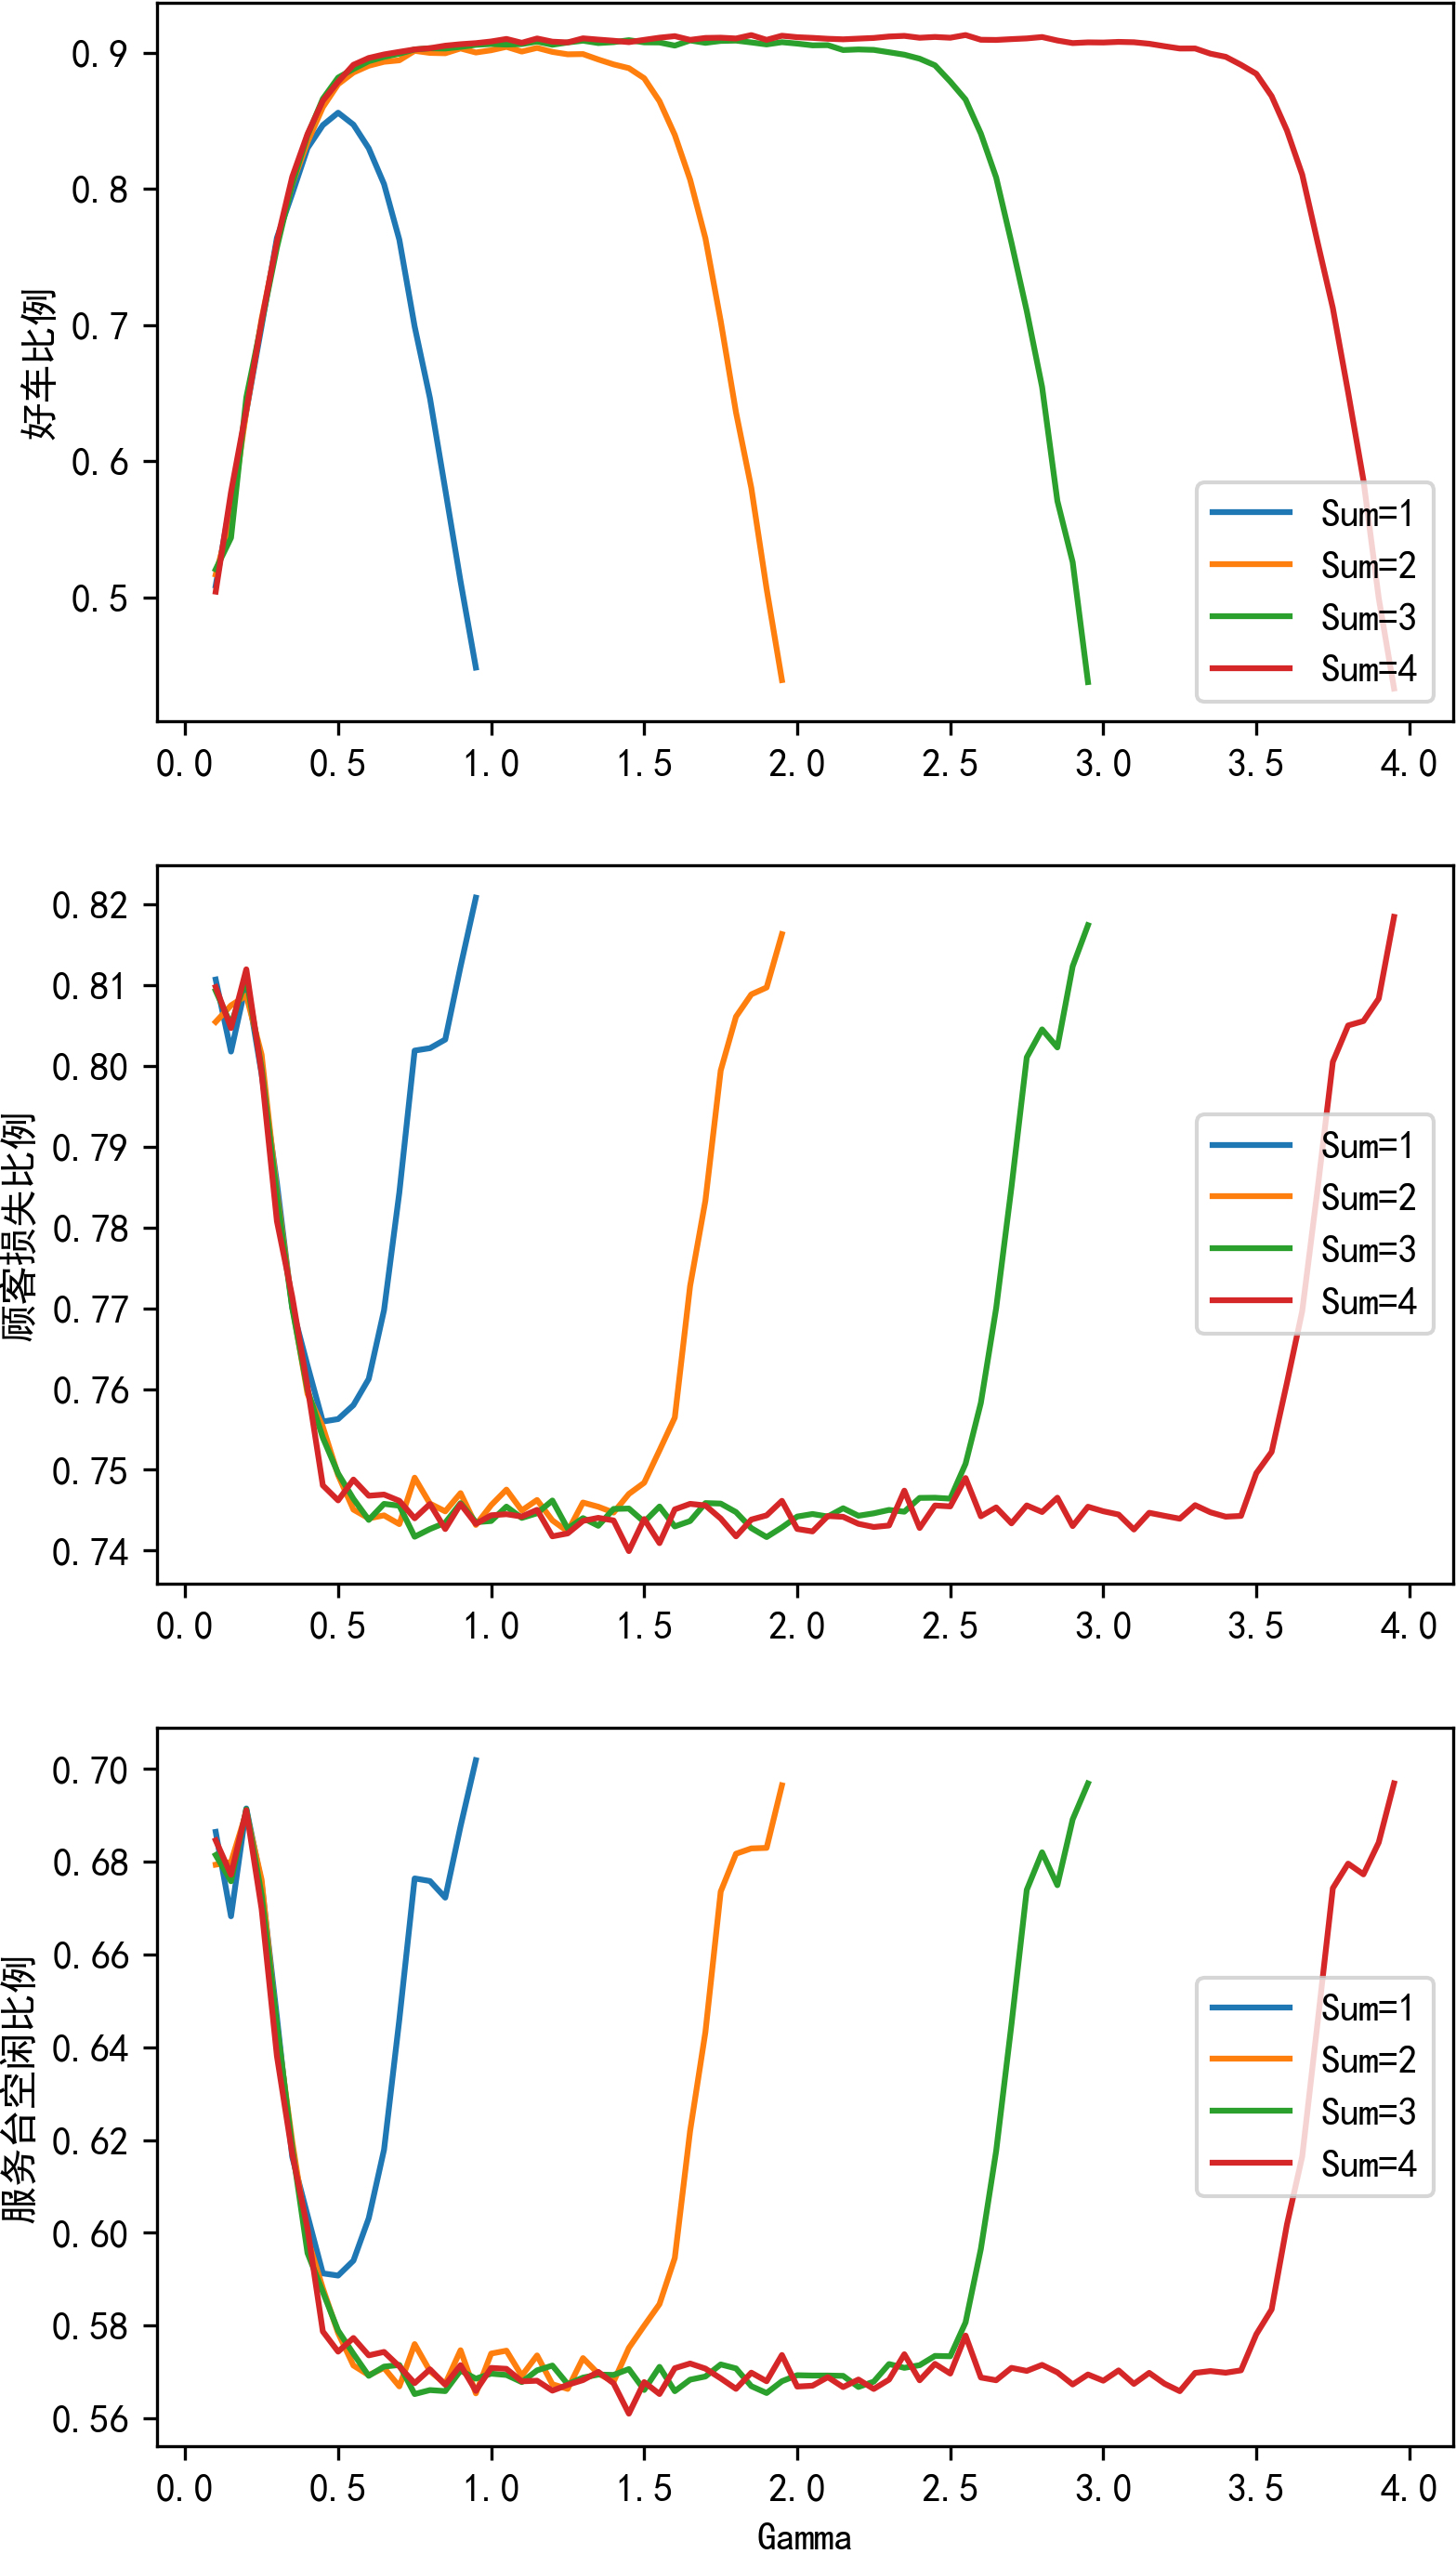
\includegraphics[width=2.3in]{Graph/perf/perfA10M50DeltaGammaSumVaryMu.png}
    %\caption{fig1}
    \end{minipage}%
    }%
    % \caption{运维能力总量有限情况}
    % \label{fig:fixsum}
\end{figure}

\begin{figure}[H]
    \centering
    \subfigure[回收与投放速度总和为定值,变动总和]{
    \begin{minipage}[t]{0.5\textwidth}
    \centering
    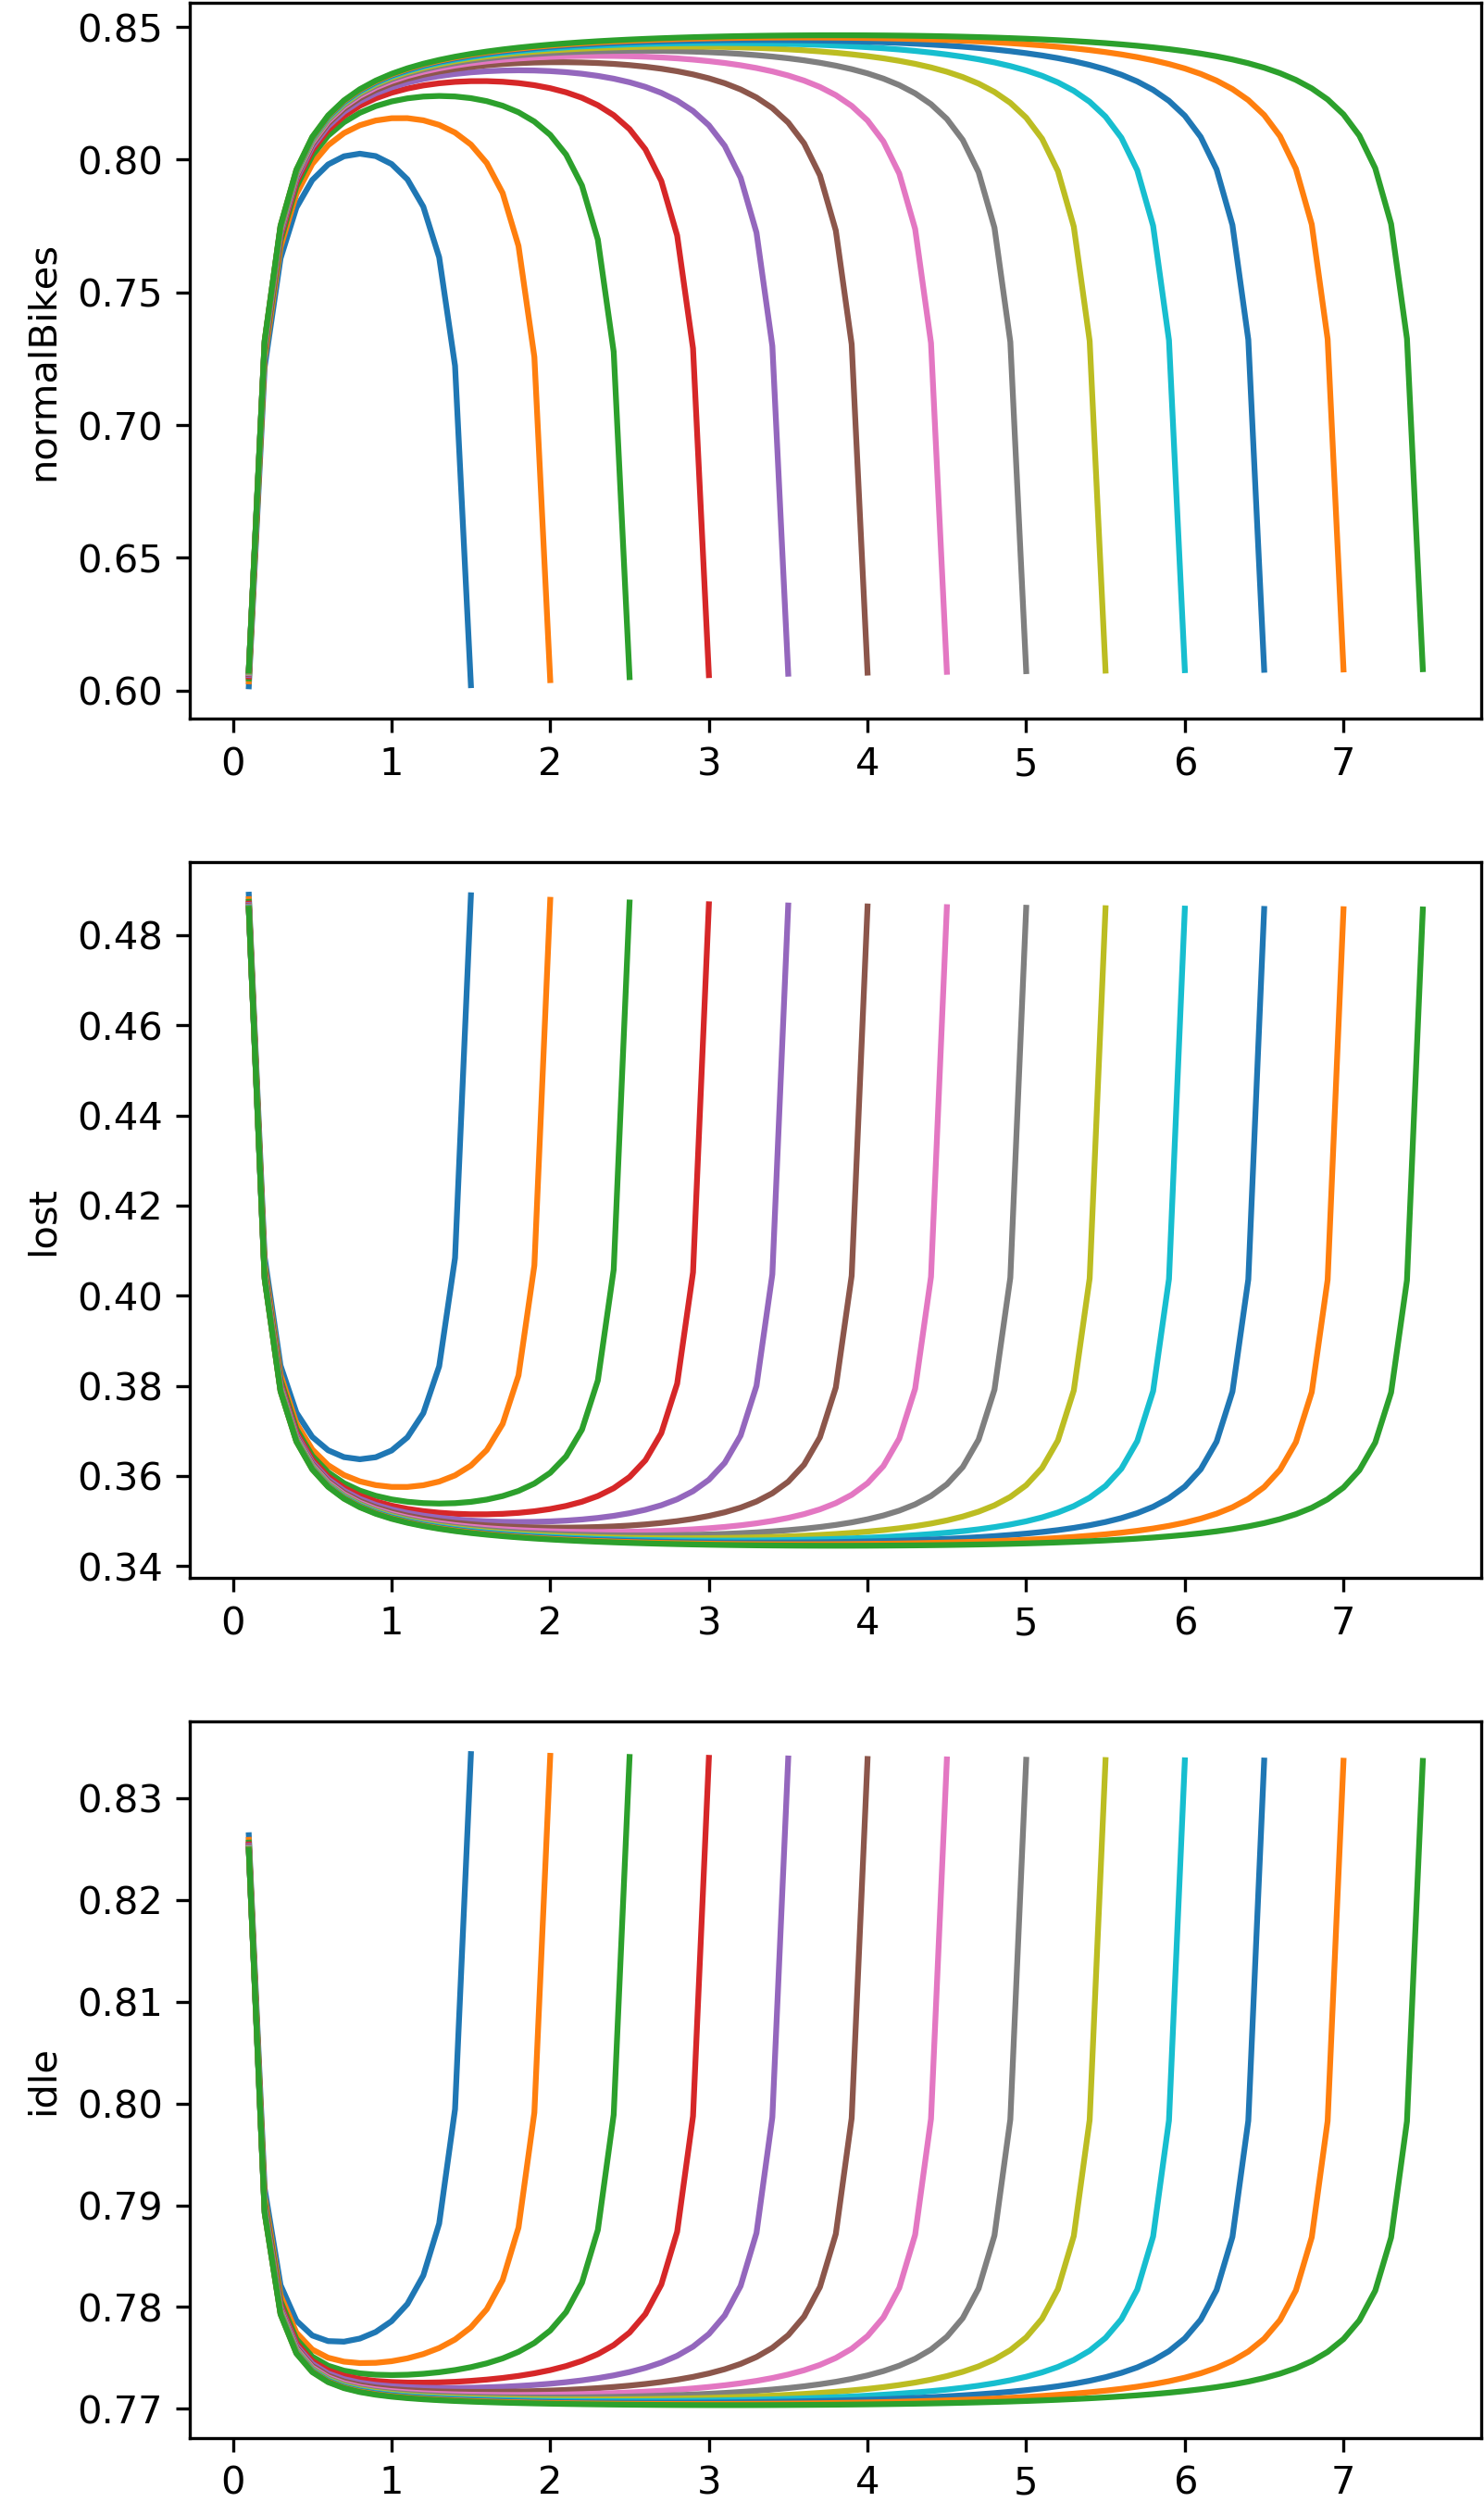
\includegraphics[width=2.4in]{Graph/perf/perfGamma+Delta0-Sum0-8lines.png}
    %\caption{fig2}
    \end{minipage}%
    }%
    \centering
    \subfigure[回收与投放速度总和为定值,变动维修速率]{
    \begin{minipage}[t]{0.5\textwidth}
    \centering
    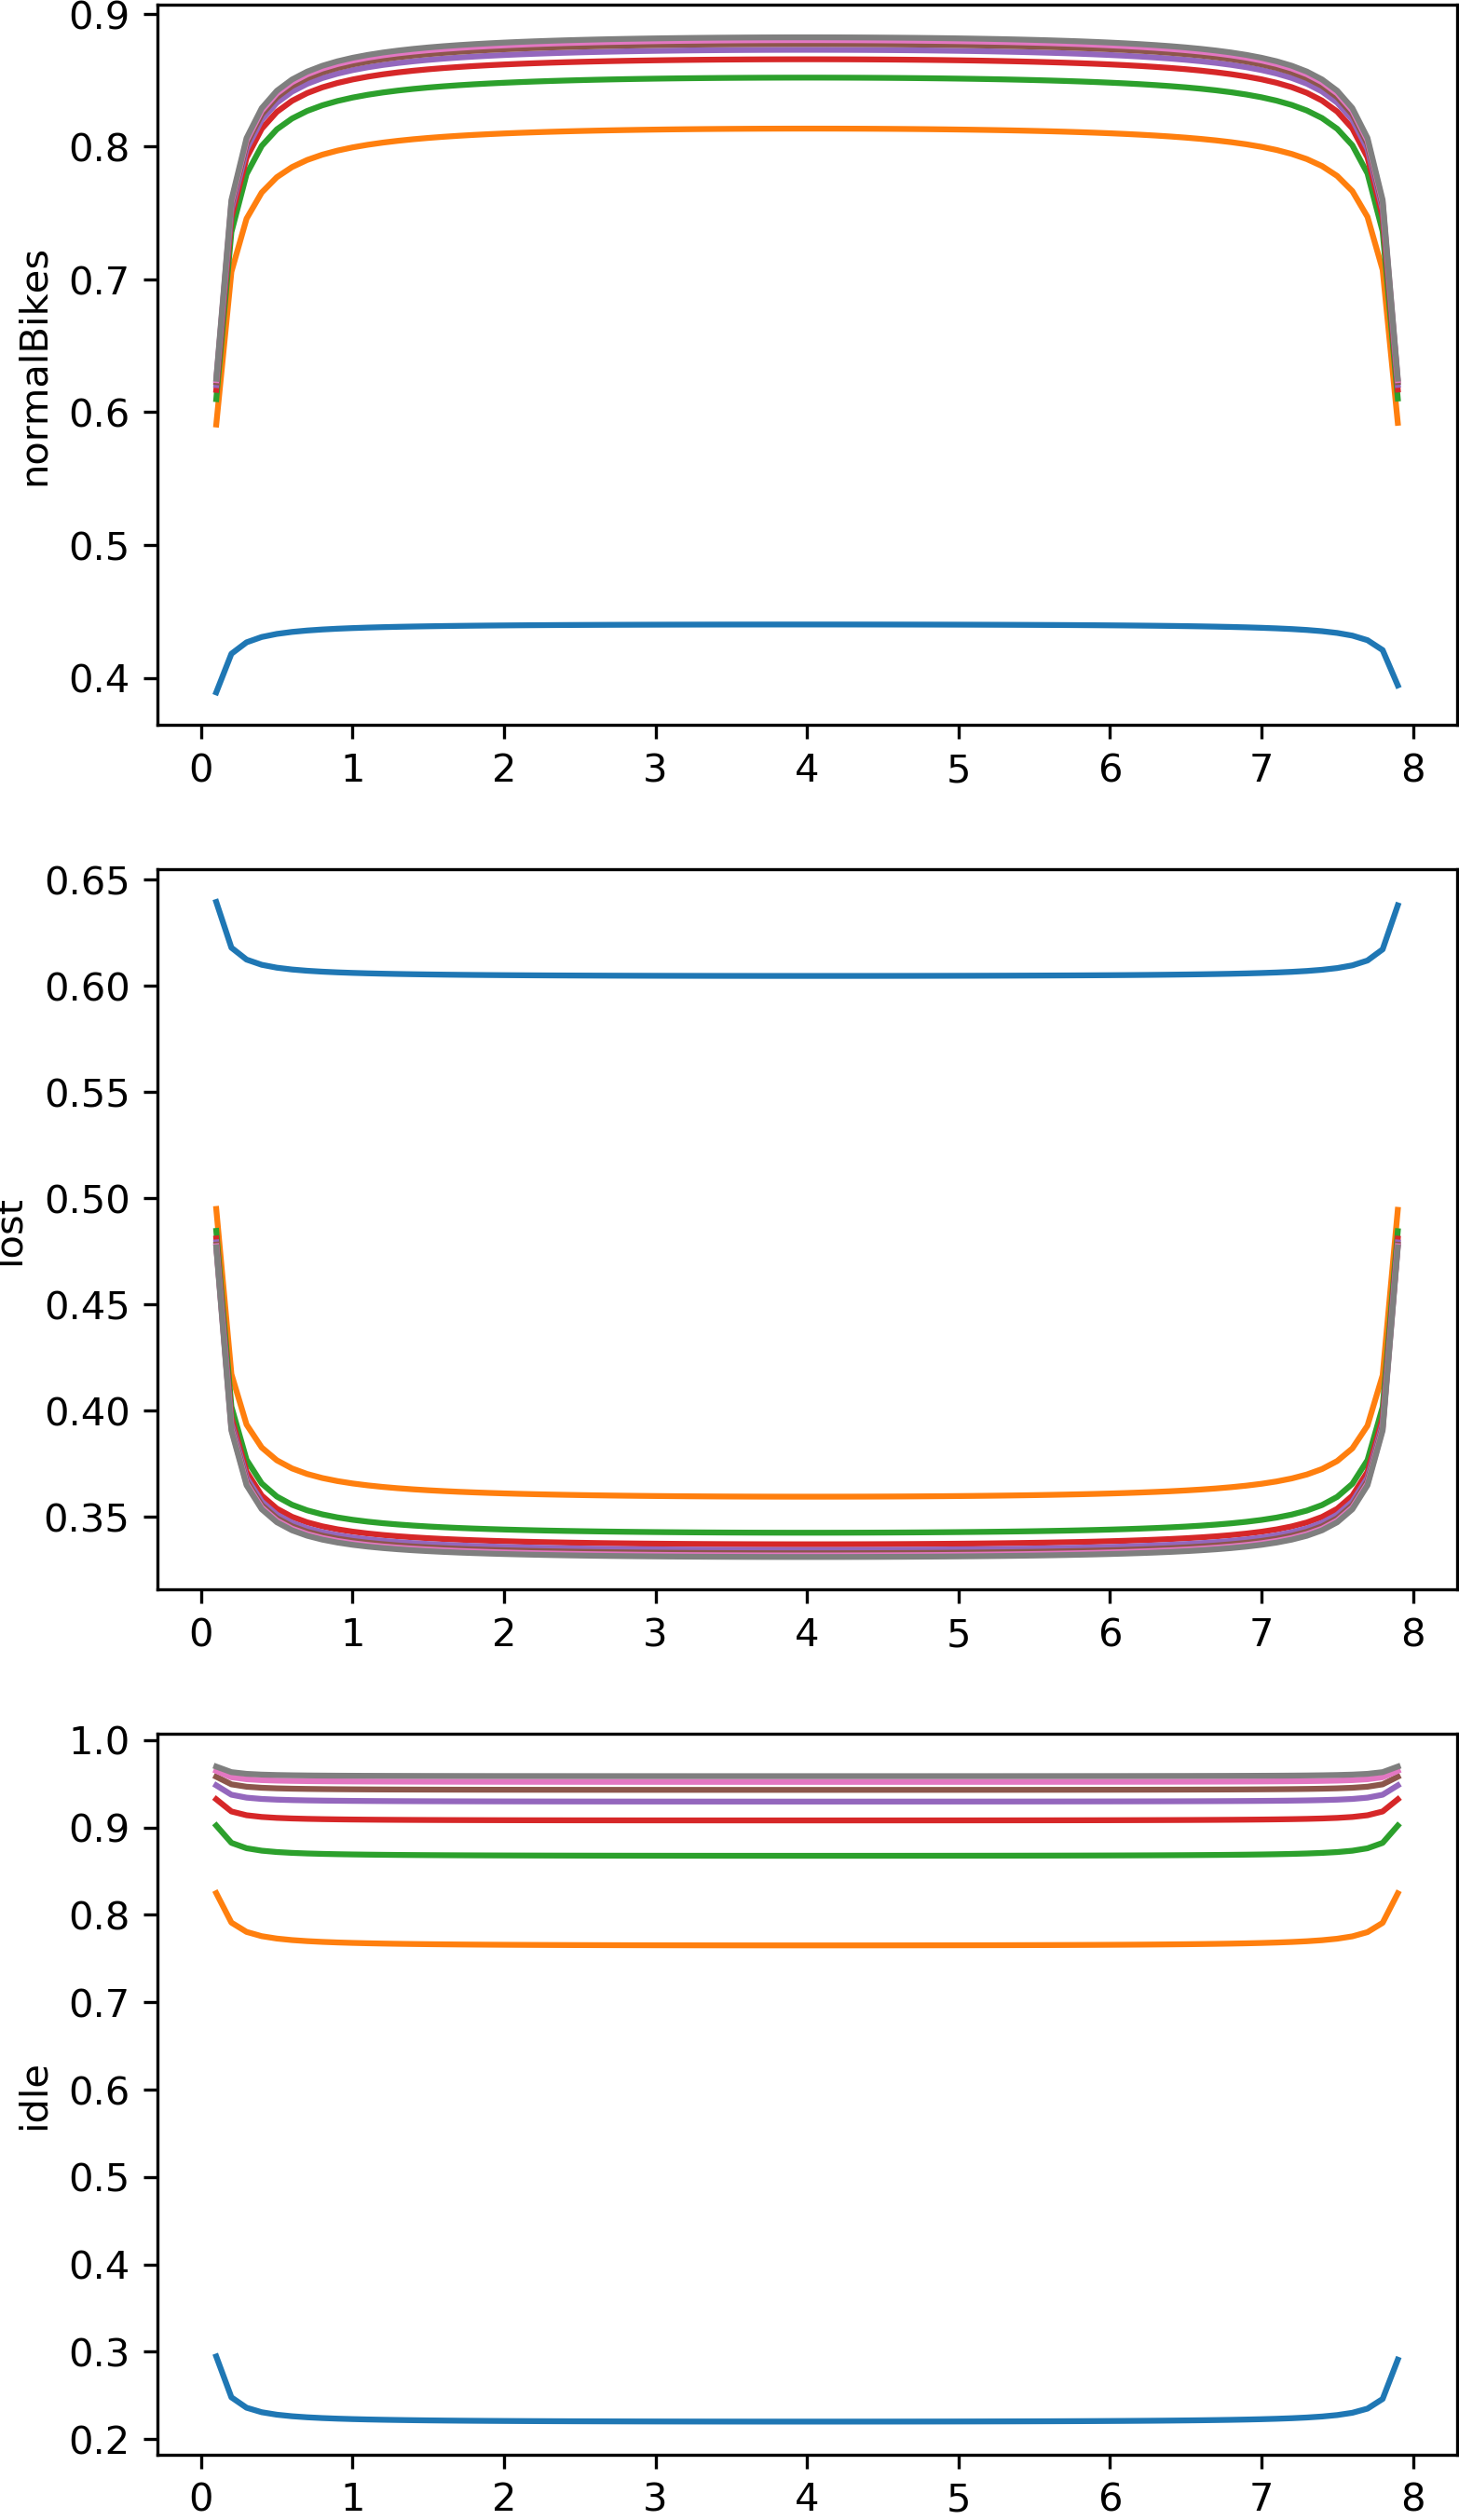
\includegraphics[width=2.3in]{Graph/perf/perfGamma+Delta0-8Mu0-4-8lines.png}
    %\caption{fig1}
    \end{minipage}%
    }%xs
    \label{fig:fixsum}
\end{figure}

\begin{figure}[H]
    \centering
    \subfigure[perfA10M50B\_-D\_1-7]{
    \begin{minipage}[t]{0.5\textwidth}
    \centering
    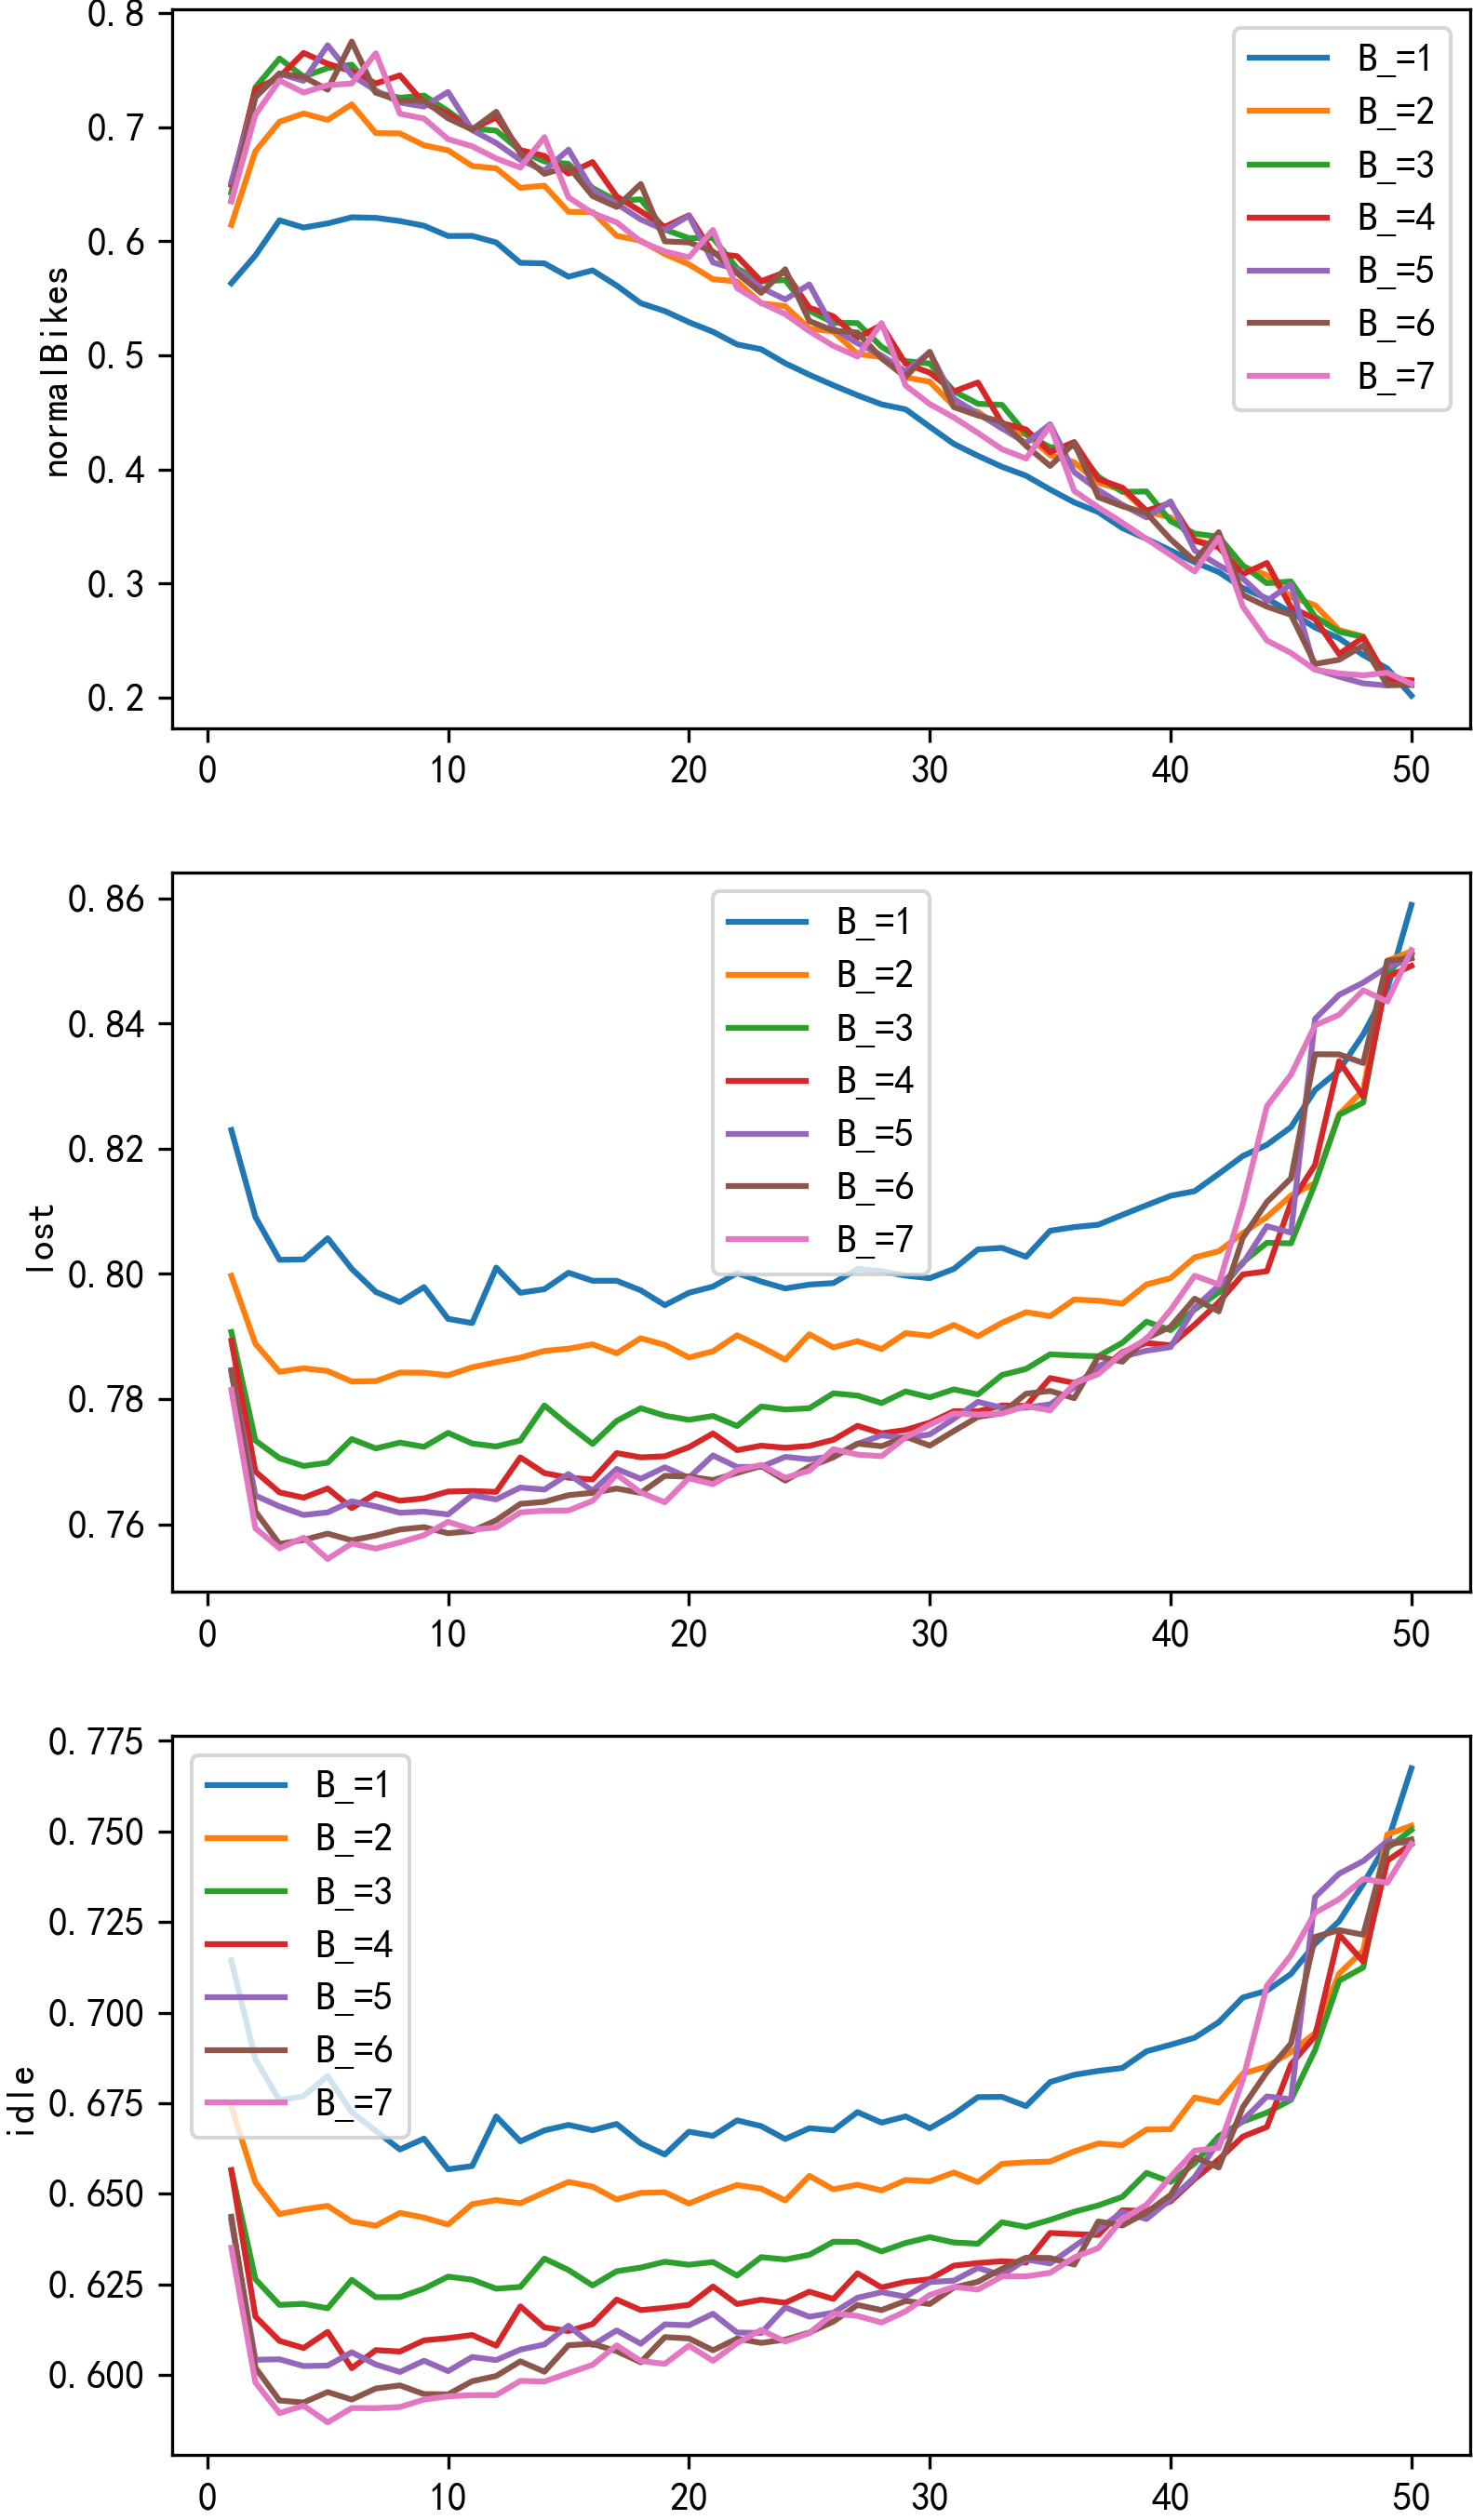
\includegraphics[width=2.3in]{Graph/perf/perfA10M50B_-D_1-7.png}
    %\caption{fig1}
    \end{minipage}%
    }%xs
    \centering
    \subfigure[A10M50N1-50Mu0-4]{
    \begin{minipage}[t]{0.5\textwidth}
    \centering
    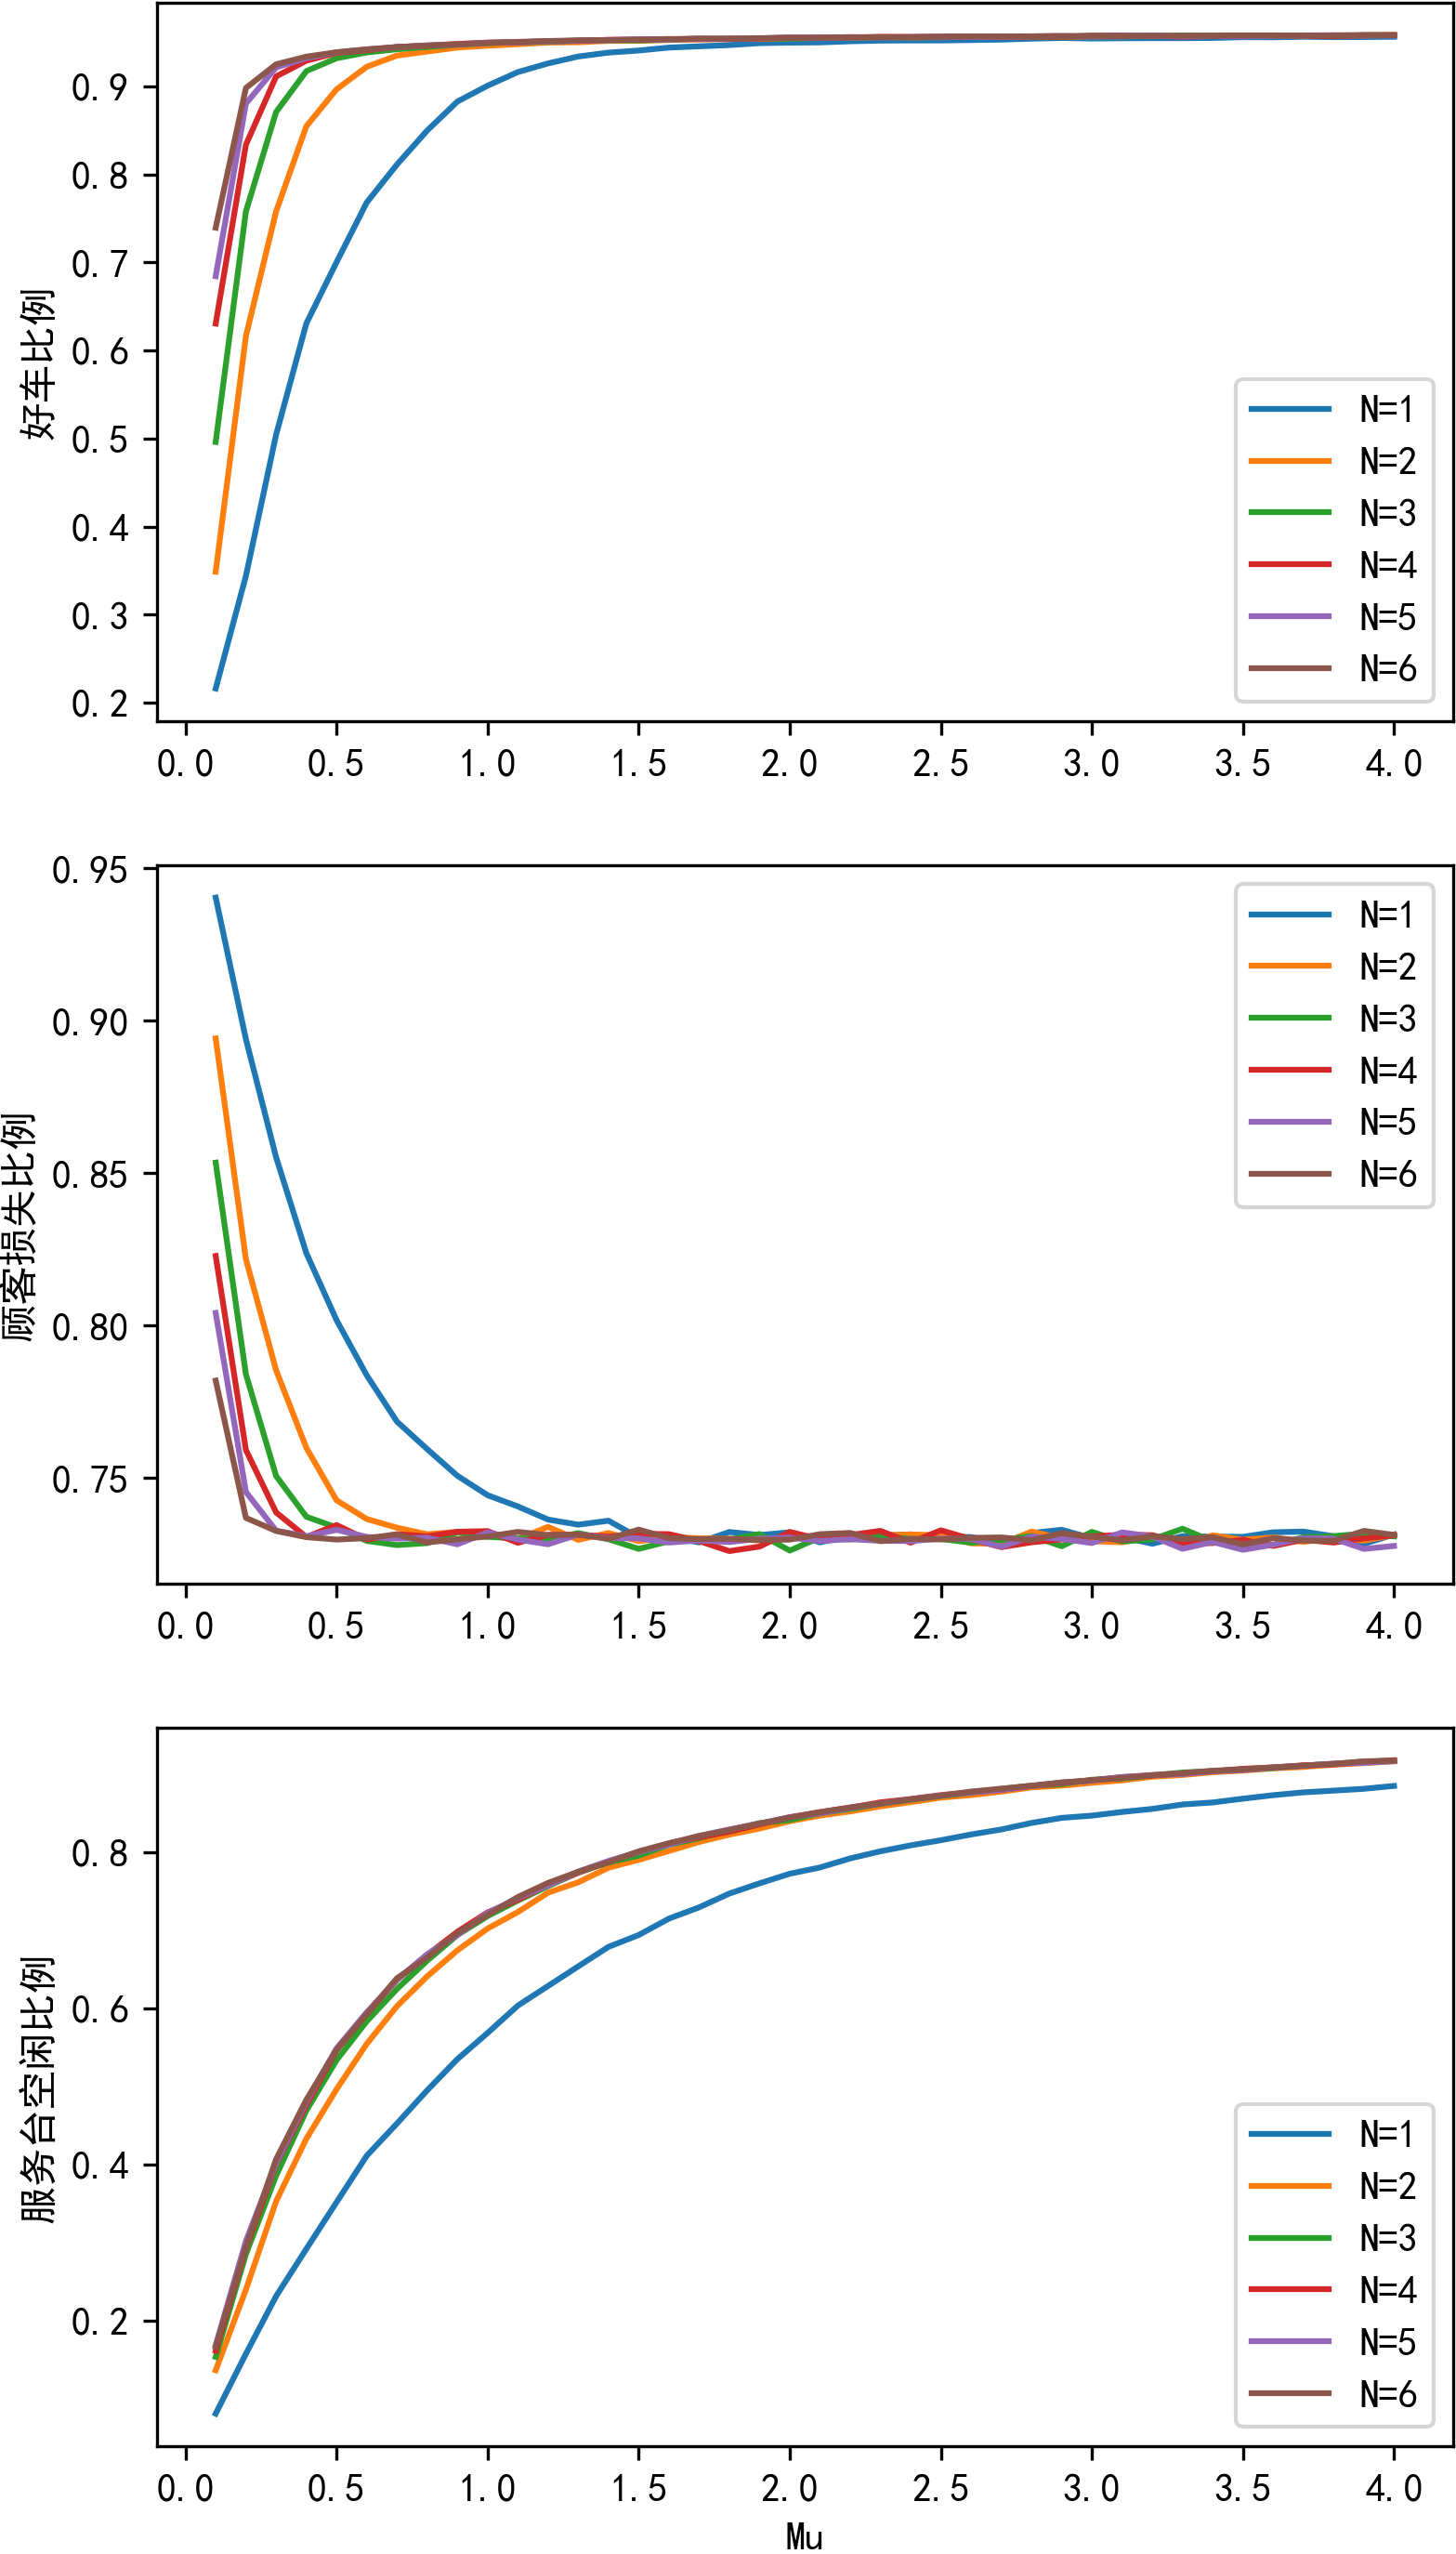
\includegraphics[width=2.3in]{Graph/perf/perfA10M50N1-50Mu0-4.png}
    %\caption{fig1}
    \end{minipage}%
    }%xs
    \caption{运维能力总量有限情况}
    \label{fig:fixsum}
\end{figure}

\begin{figure}[H]
    \centering
    \subfigure[A10M50D\_1-50Delta0-4]{
    \begin{minipage}[t]{0.5\textwidth}
    \centering
    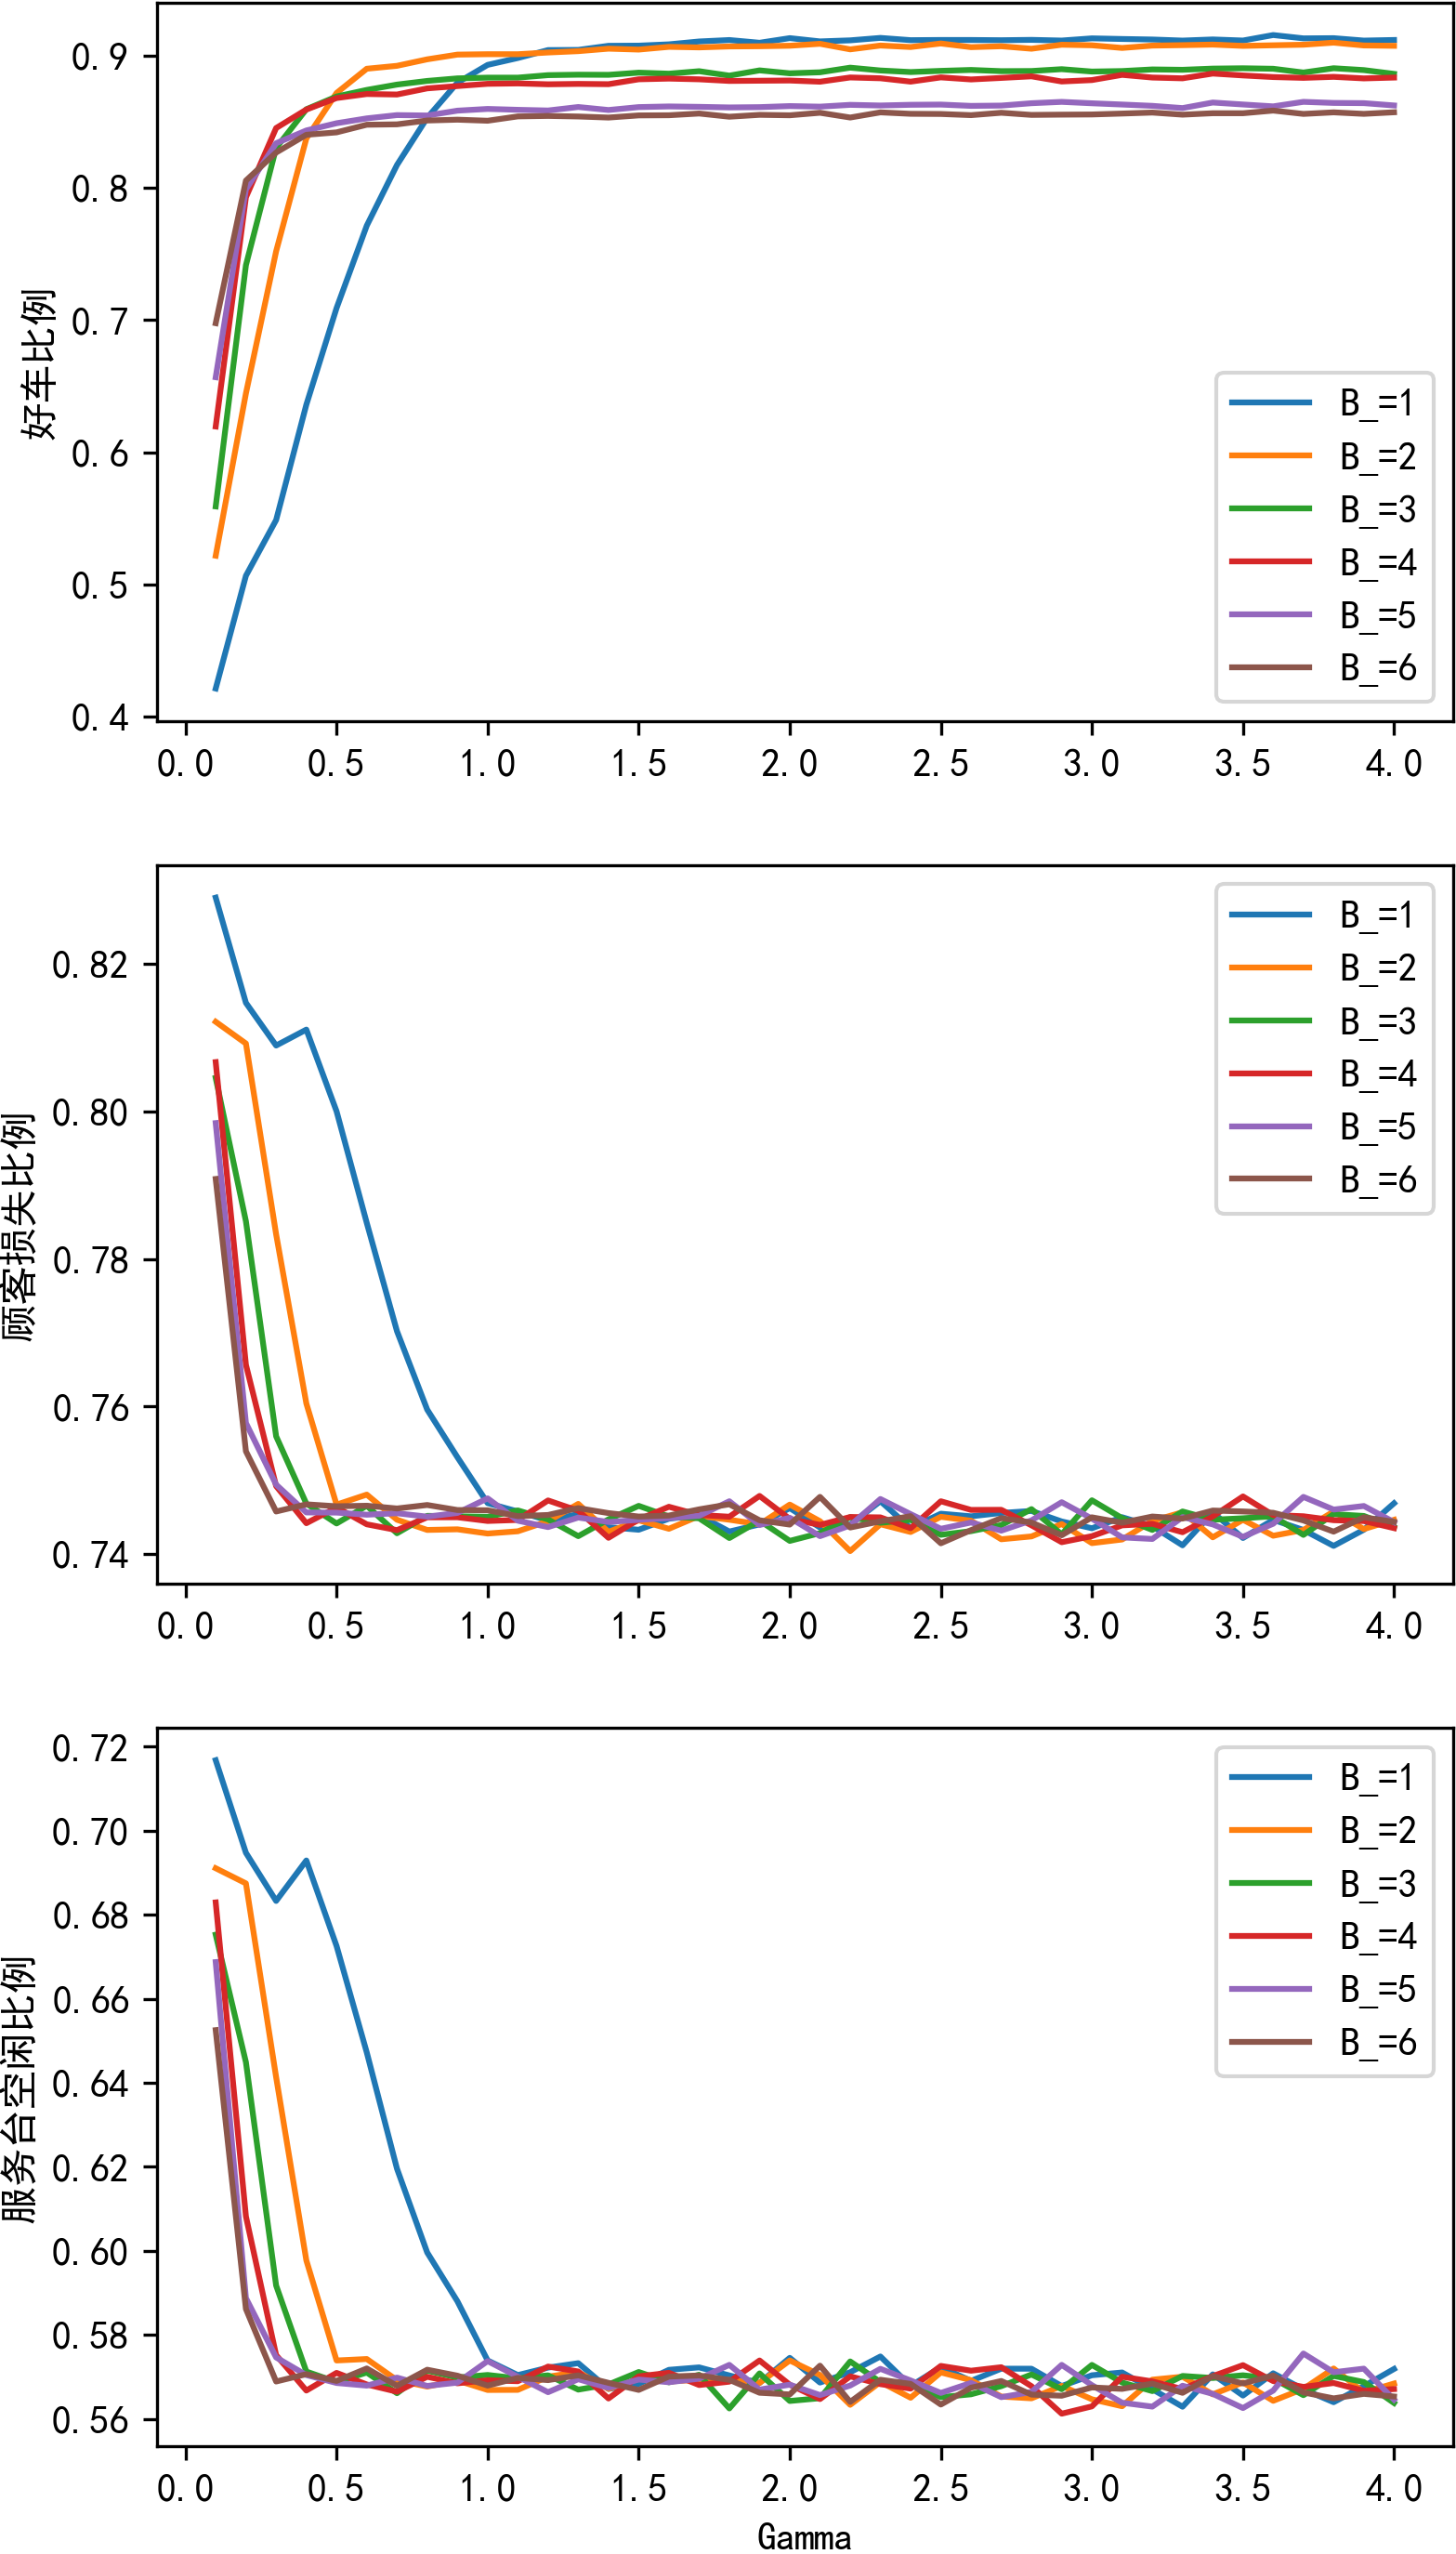
\includegraphics[width=2.3in]{Graph/perf/perfA10M50D_1-50Delta0-4.png}
    %\caption{fig1}
    \end{minipage}%
    }%xs
    \centering
    \subfigure[A10M50B\_1-6Gamma0-4]{
    \begin{minipage}[t]{0.5\textwidth}
    \centering
    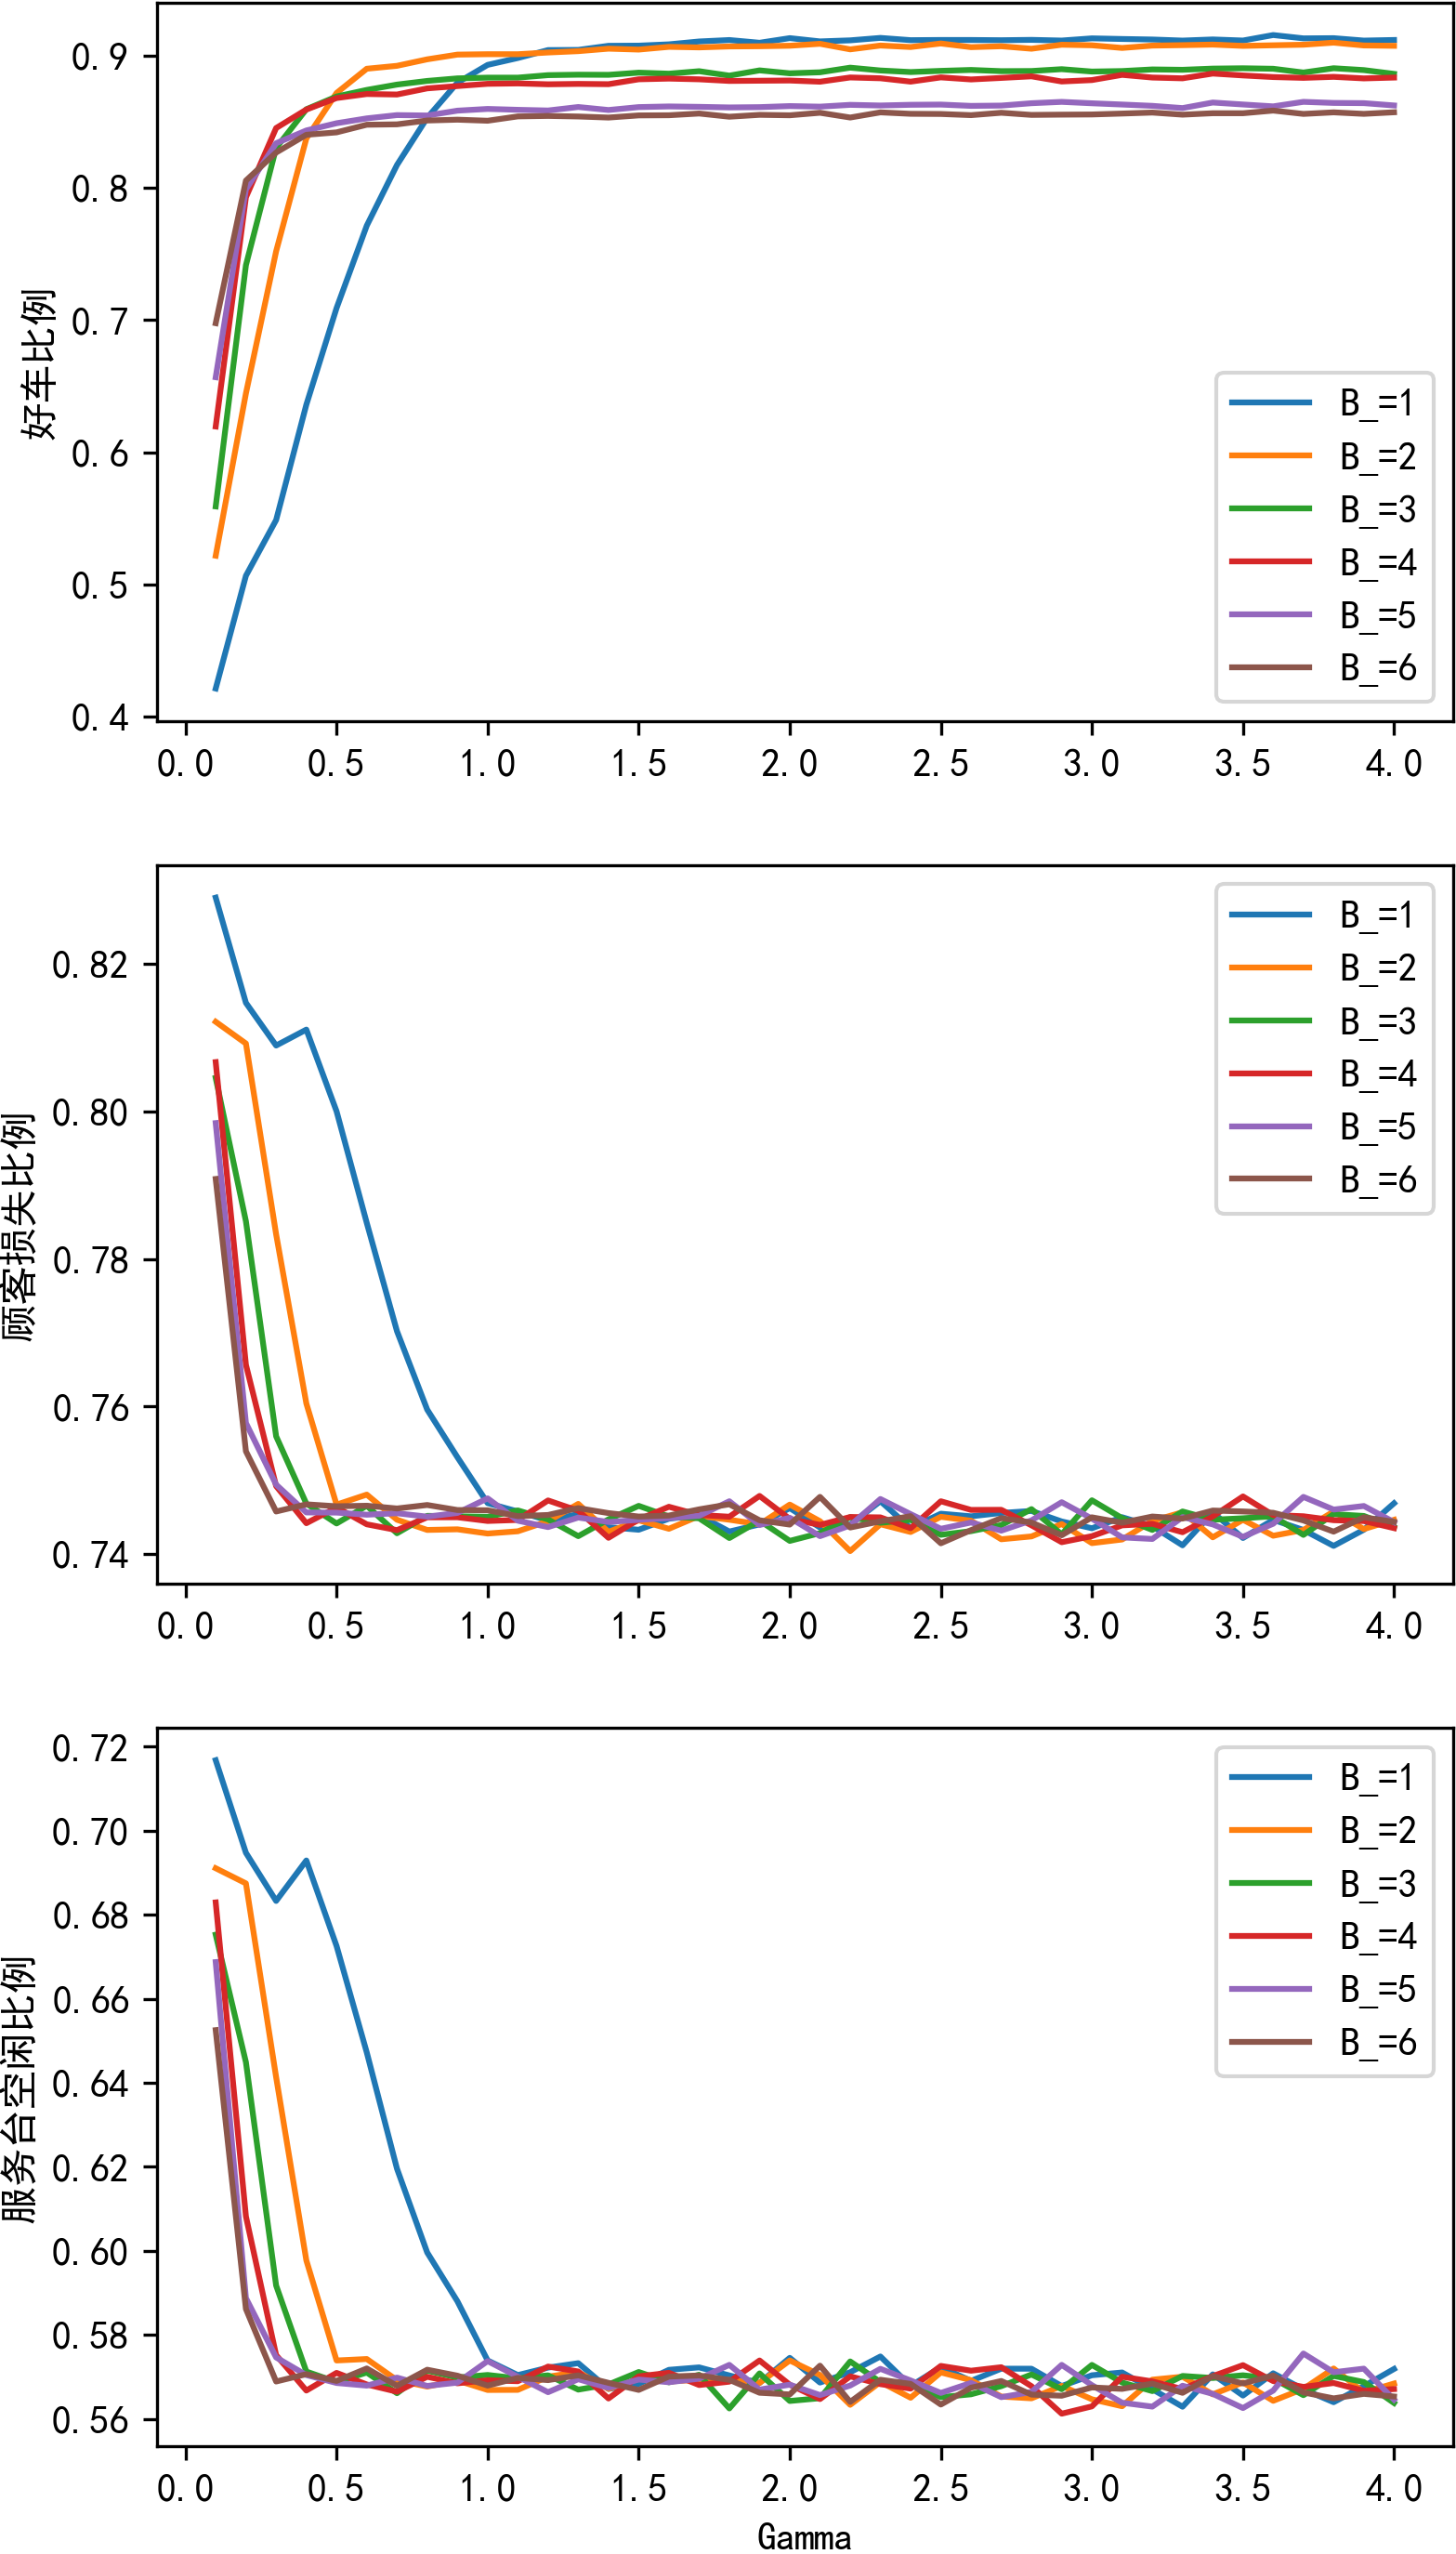
\includegraphics[width=2.3in]{Graph/perf/perfA10M50B_1-6Gamma0-4.png}
    %\caption{fig1}
    \end{minipage}%
    }%xs
    \caption{运维能力总量有限情况}
    \label{fig:fixsum}
\end{figure}

\end{document}

% \newgeometry{left=0.1cm,right=0.1cm, top=0.1cm, bottom=0.1cm}
% \begin{figure}[h]
%     \centering
%     \subfigure[Gamma]{
%     \begin{minipage}[t]{0.5\linewidth}
%     \centering
%     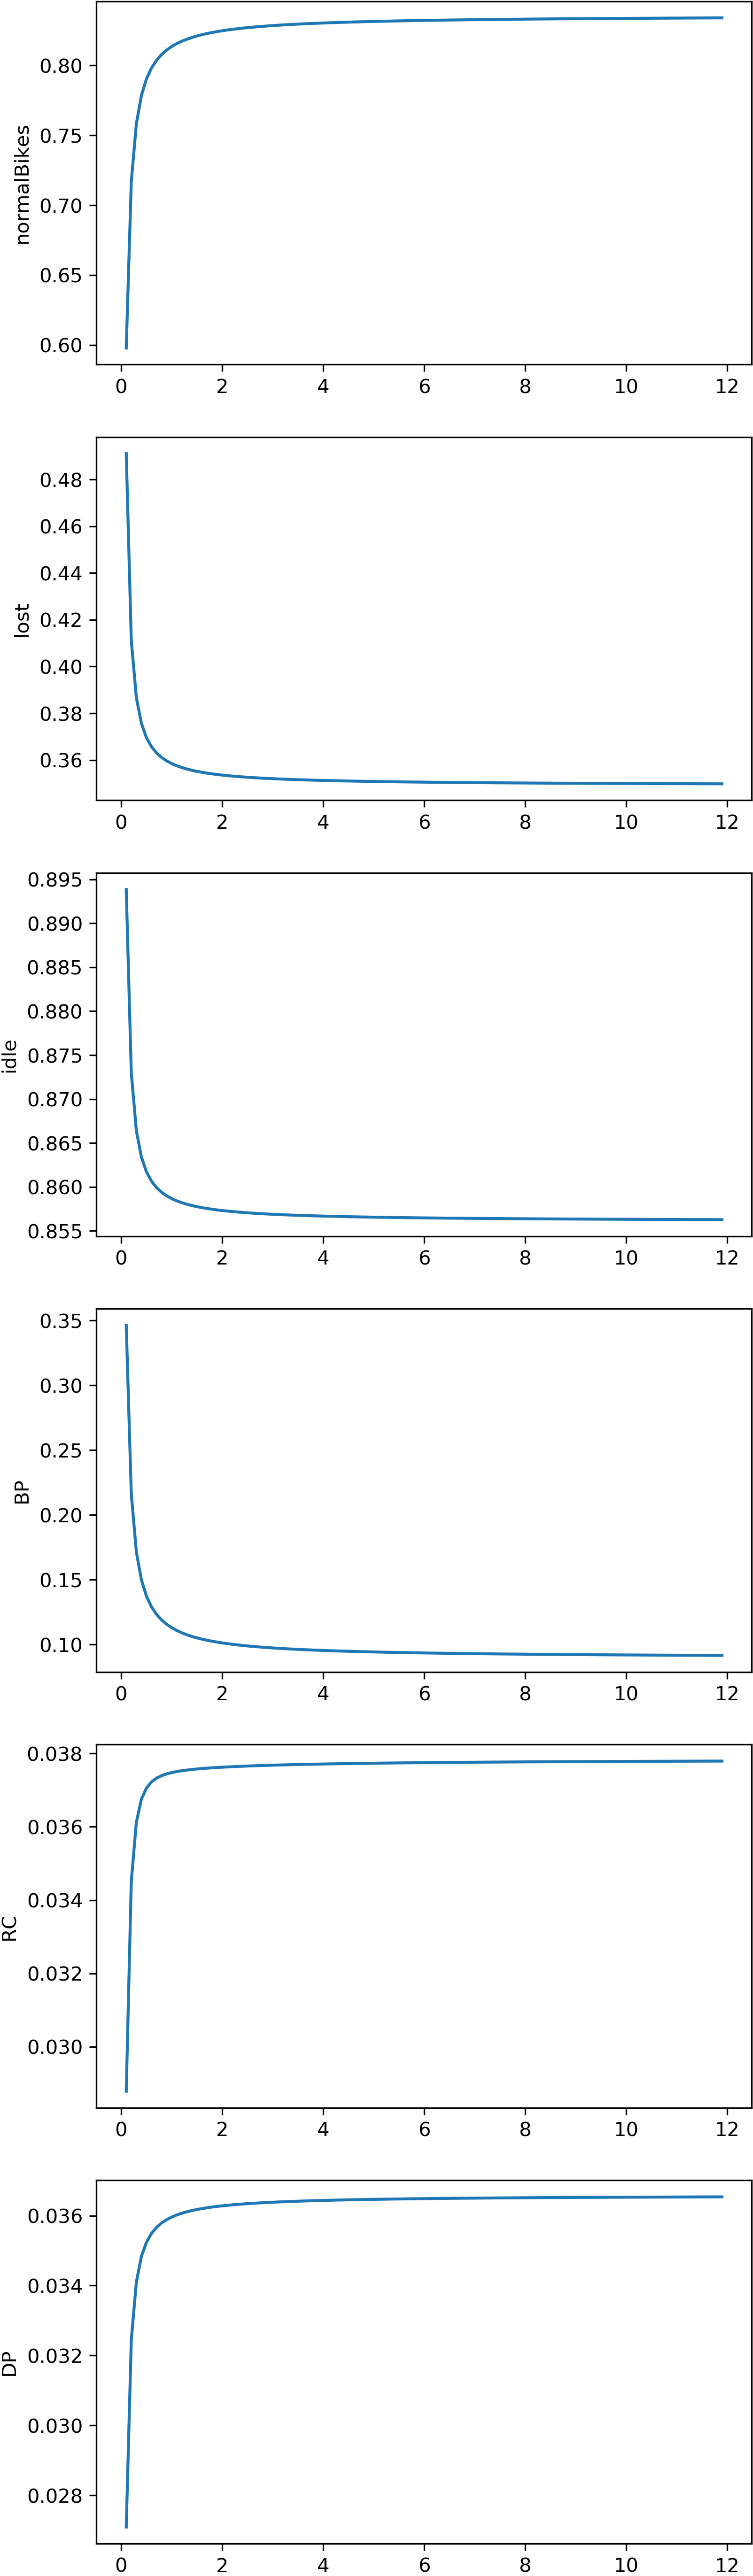
\includegraphics[width=2.3in]{Graph/perfGamma0-12.png}
%     %\caption{fig1}
%     \end{minipage}%
%     }%
%     \centering
%     \subfigure[$\overline{B}$]{
%     \begin{minipage}[t]{0.5\linewidth}
%     \centering
%     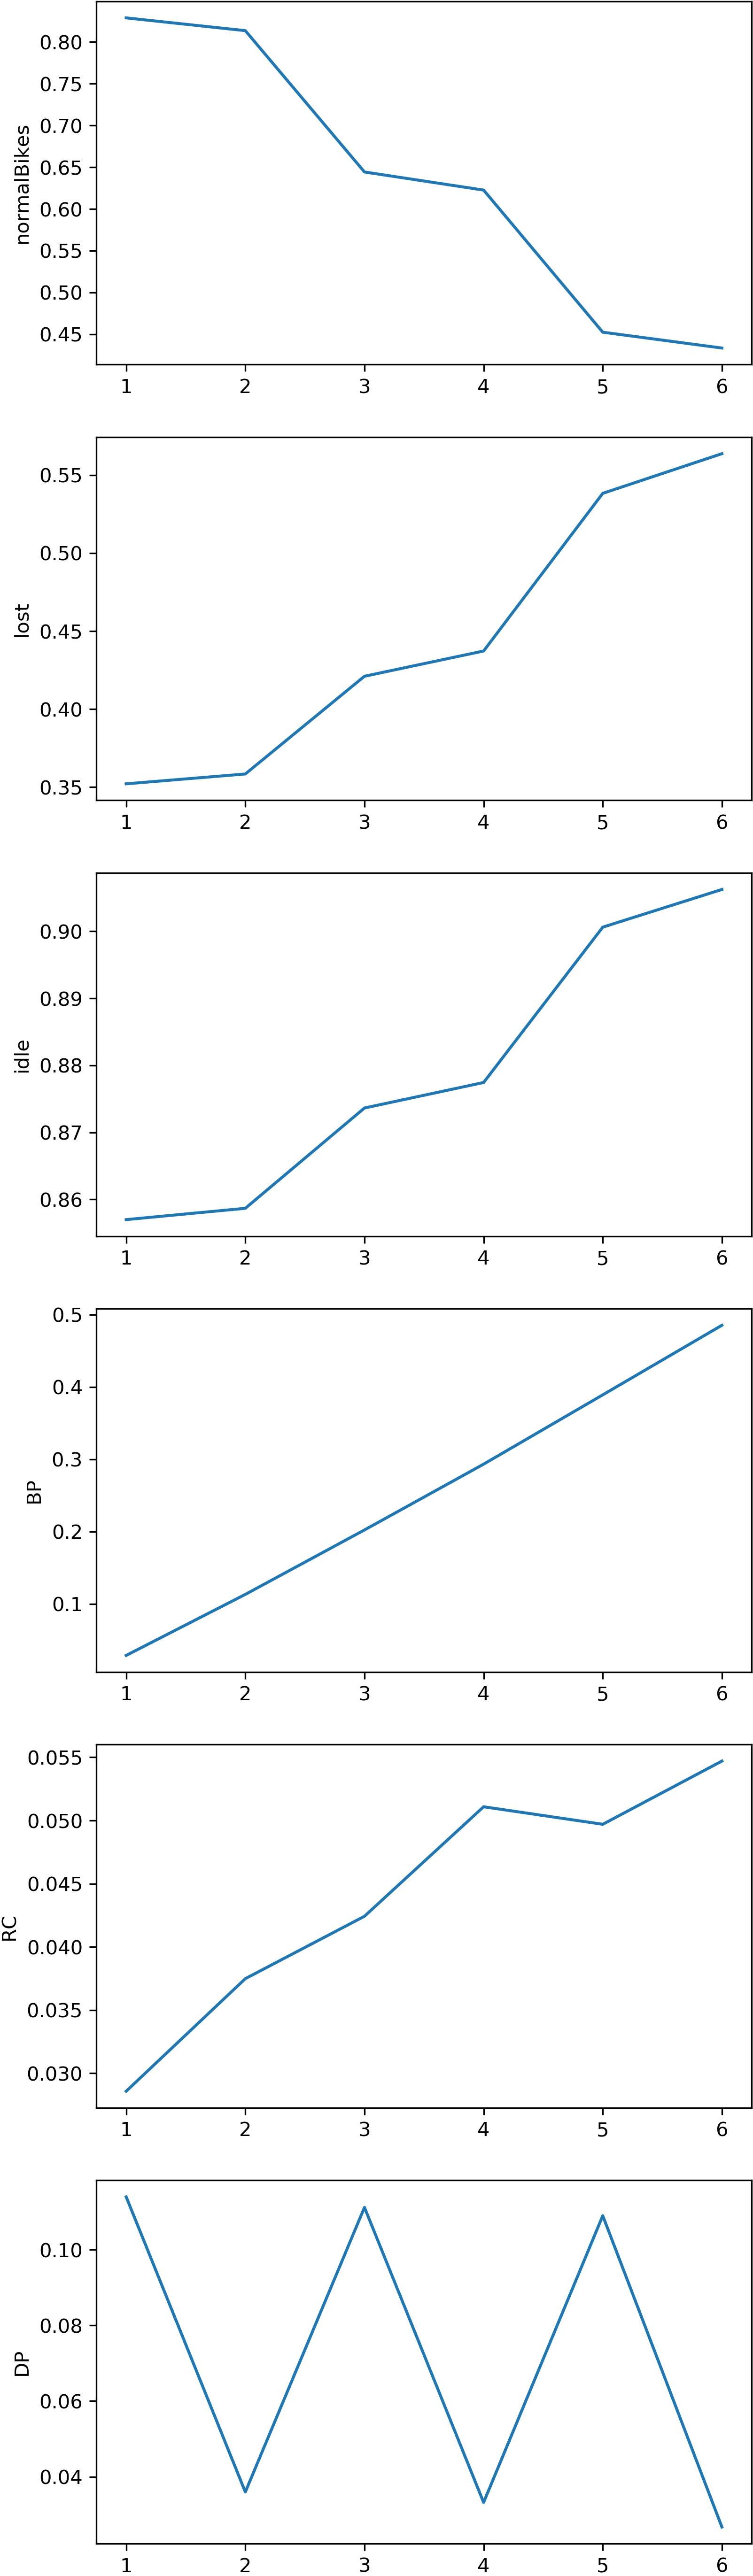
\includegraphics[width=2.3in]{Graph/perfB_1-6.png}
%     %\caption{fig2}
%     \end{minipage}%
%     }%
% \end{figure}
% \restoregeometry

% \newgeometry{left=0.1cm,right=0.1cm, top=0.1cm, bottom=0.1cm}
% \begin{figure}[h]
%     \centering
%     \subfigure[Mu]{
%     \begin{minipage}[t]{0.5\linewidth}
%     \centering
%     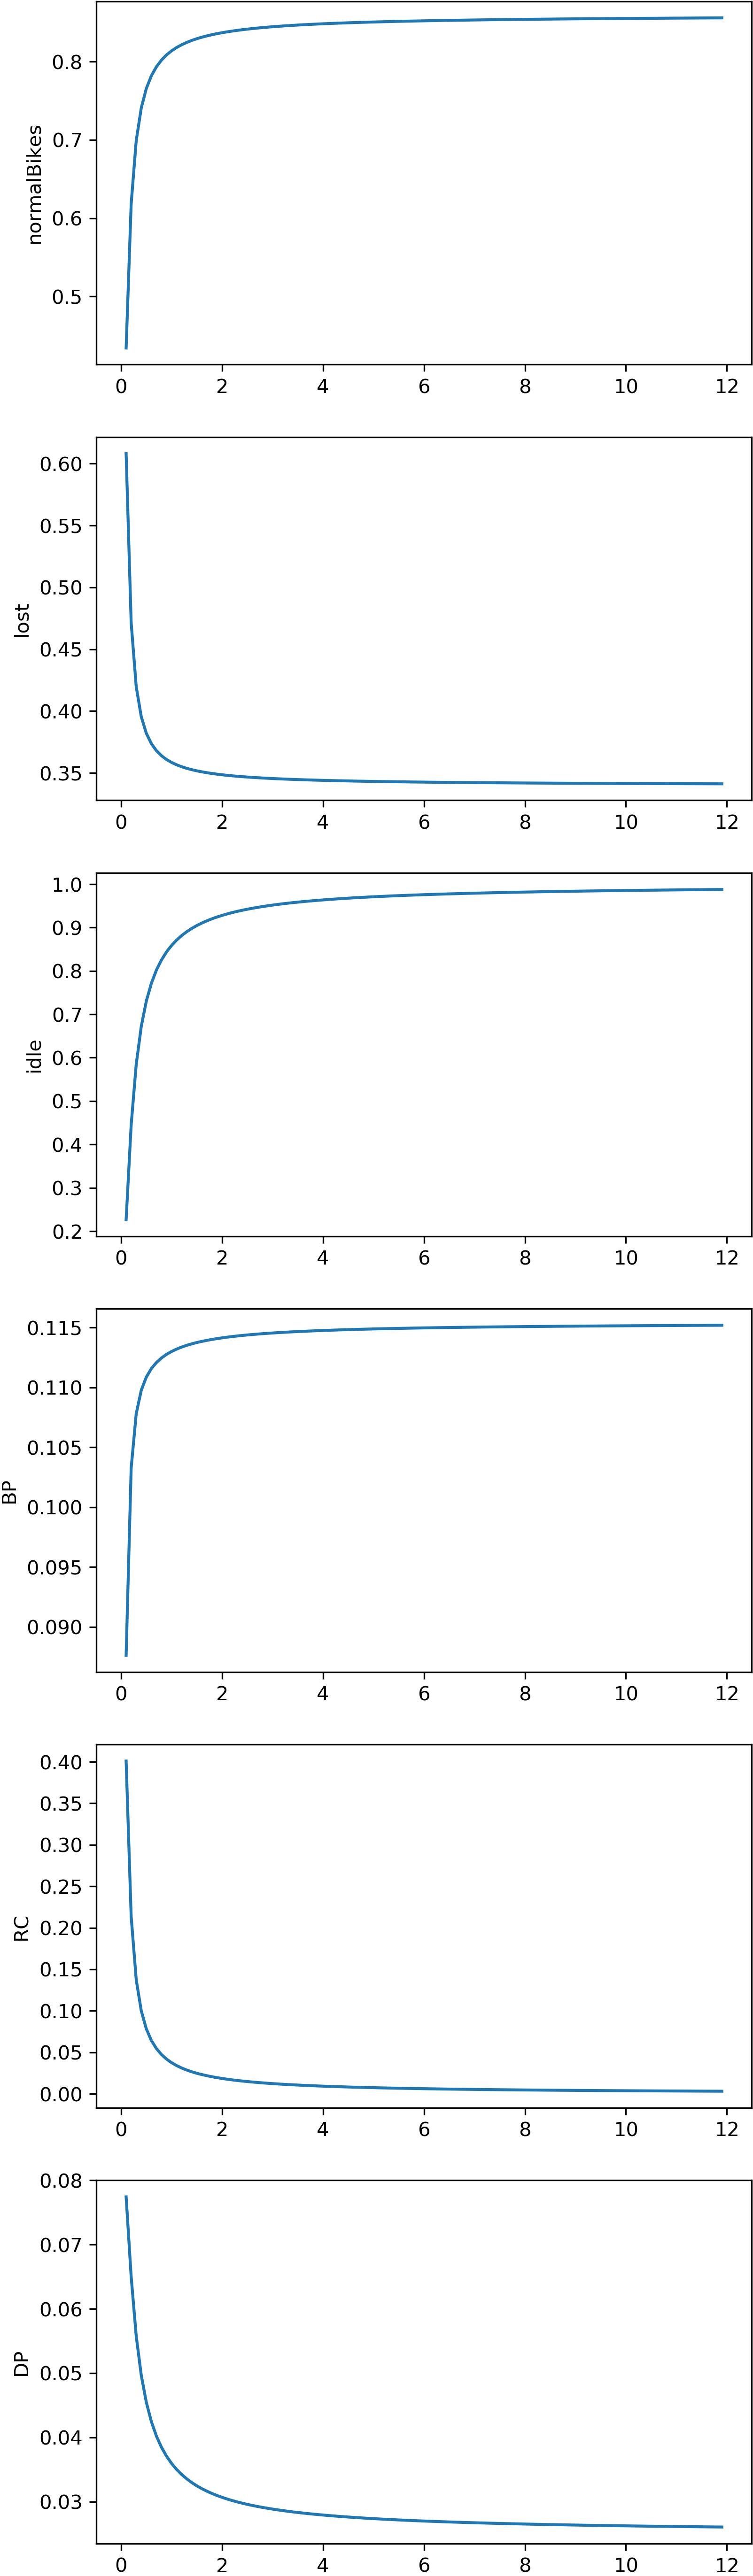
\includegraphics[width=2.3in]{Graph/perfMu0-12.png}
%     %\caption{fig1}
%     \end{minipage}%
%     }%
%     \centering
%     \subfigure[N]{
%     \begin{minipage}[t]{0.5\linewidth}
%     \centering
%     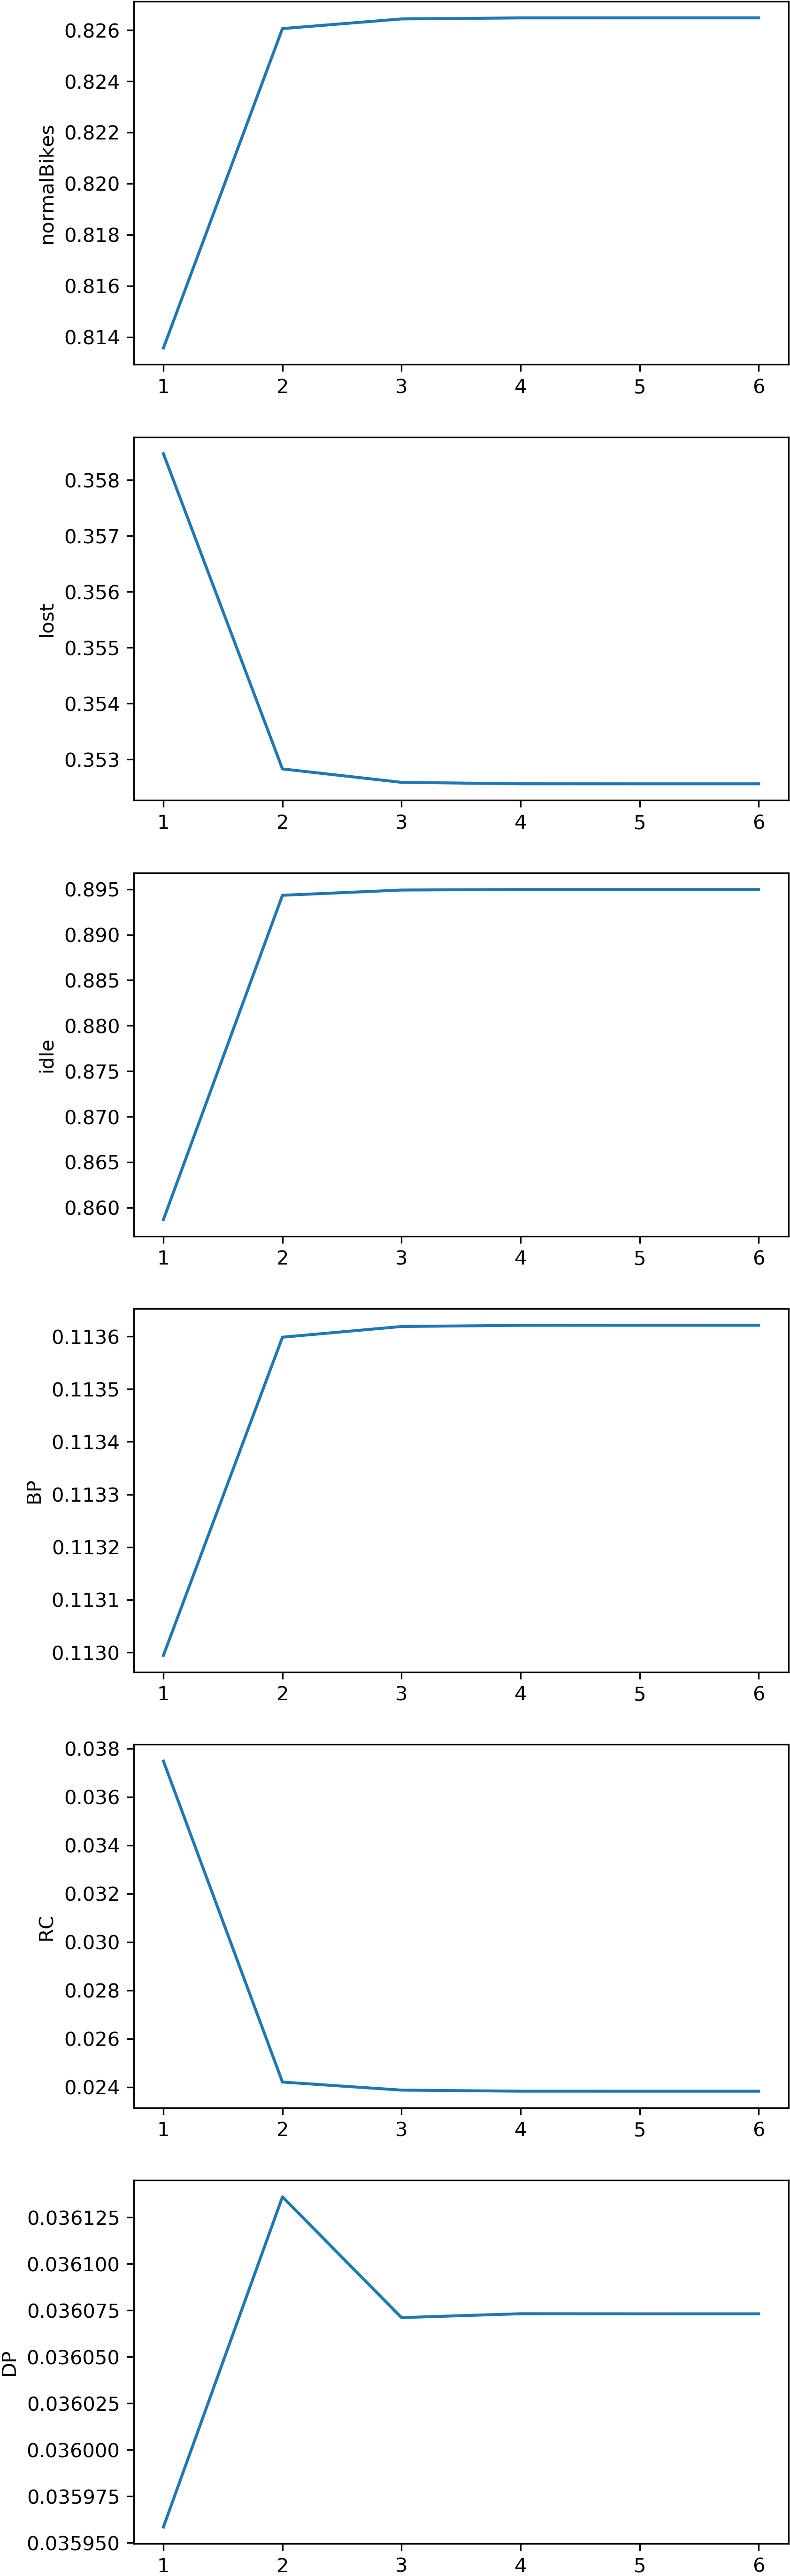
\includegraphics[width=2.3in]{Graph/perfN1-6.png}
%     %\caption{fig2}
%     \end{minipage}%
%     }%
% \end{figure}
% \restoregeometry

% \newgeometry{left=0.1cm,right=0.1cm, top=0.1cm, bottom=0.1cm}
% \begin{figure}[h]
%     \centering
%     \subfigure[Delta]{
%     \begin{minipage}[t]{0.5\linewidth}
%     \centering
%     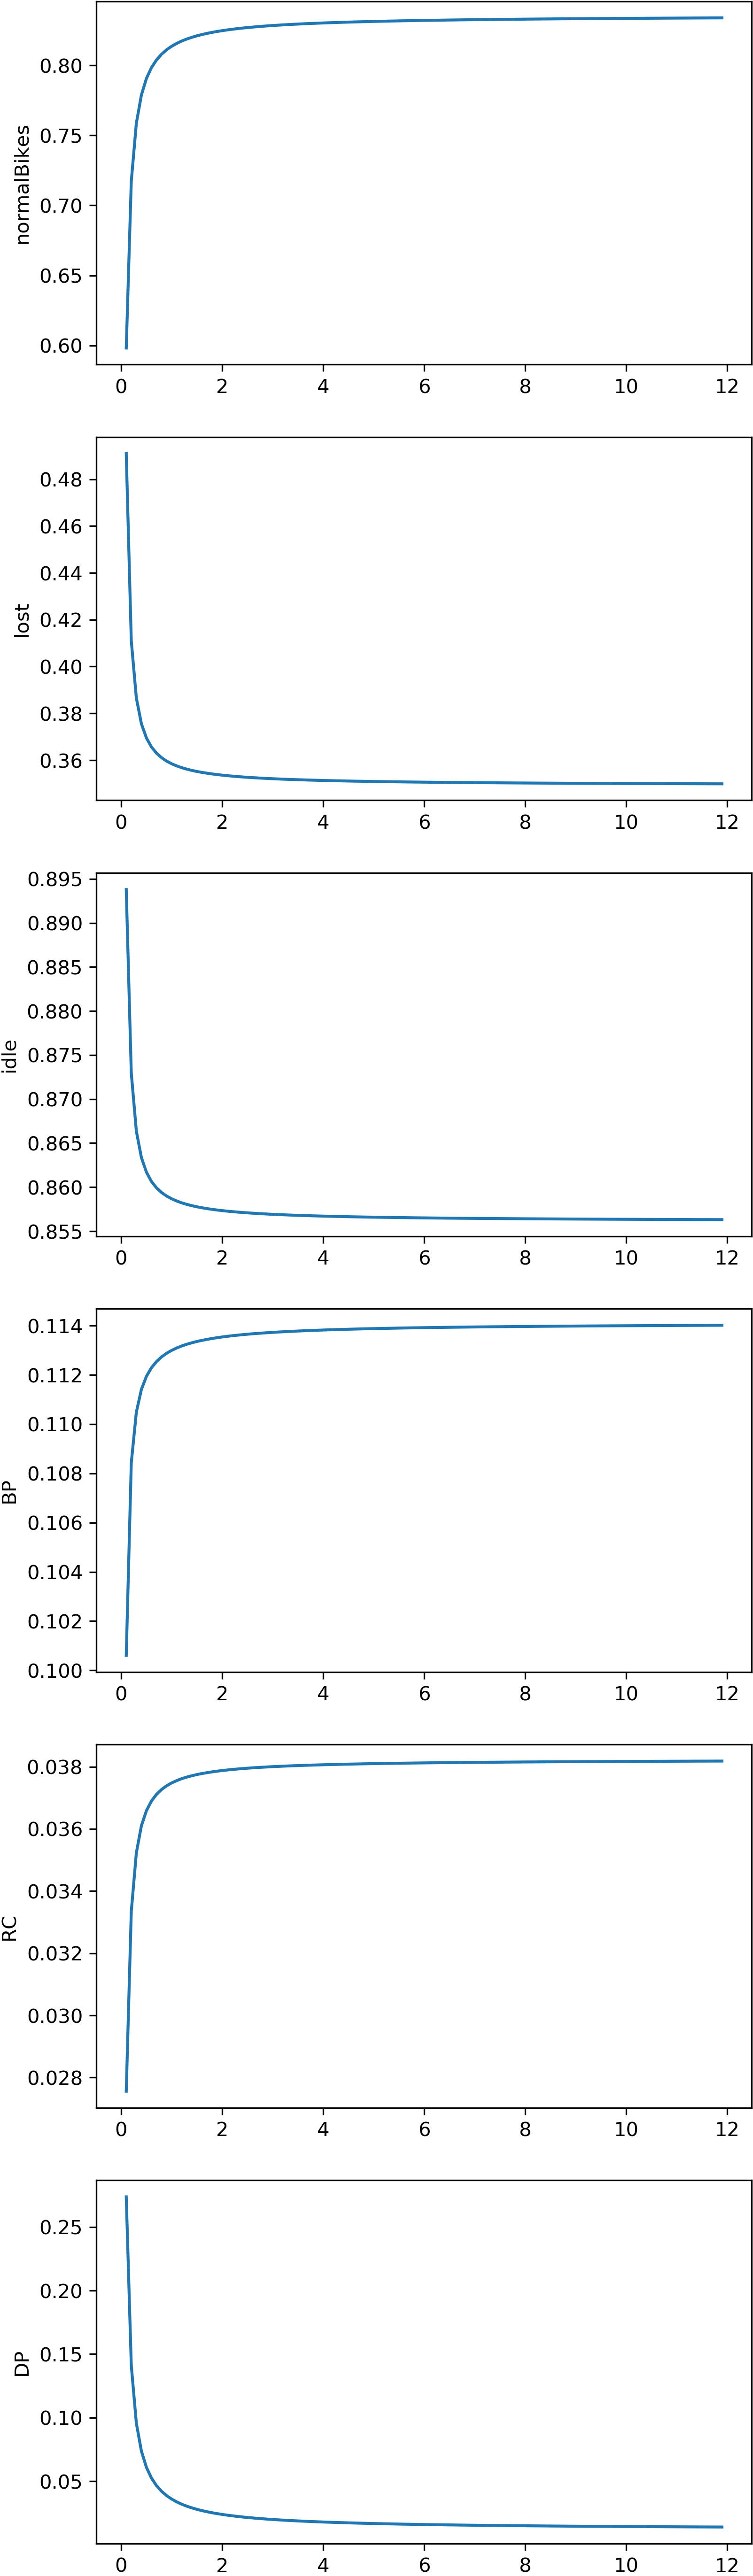
\includegraphics[width=2.3in]{Graph/perfDelta0-12.png}
%     %\caption{fig1}
%     \end{minipage}%
%     }%
%     \centering
%     \subfigure[$\overline{D}$]{
%     \begin{minipage}[t]{0.5\linewidth}
%     \centering
%     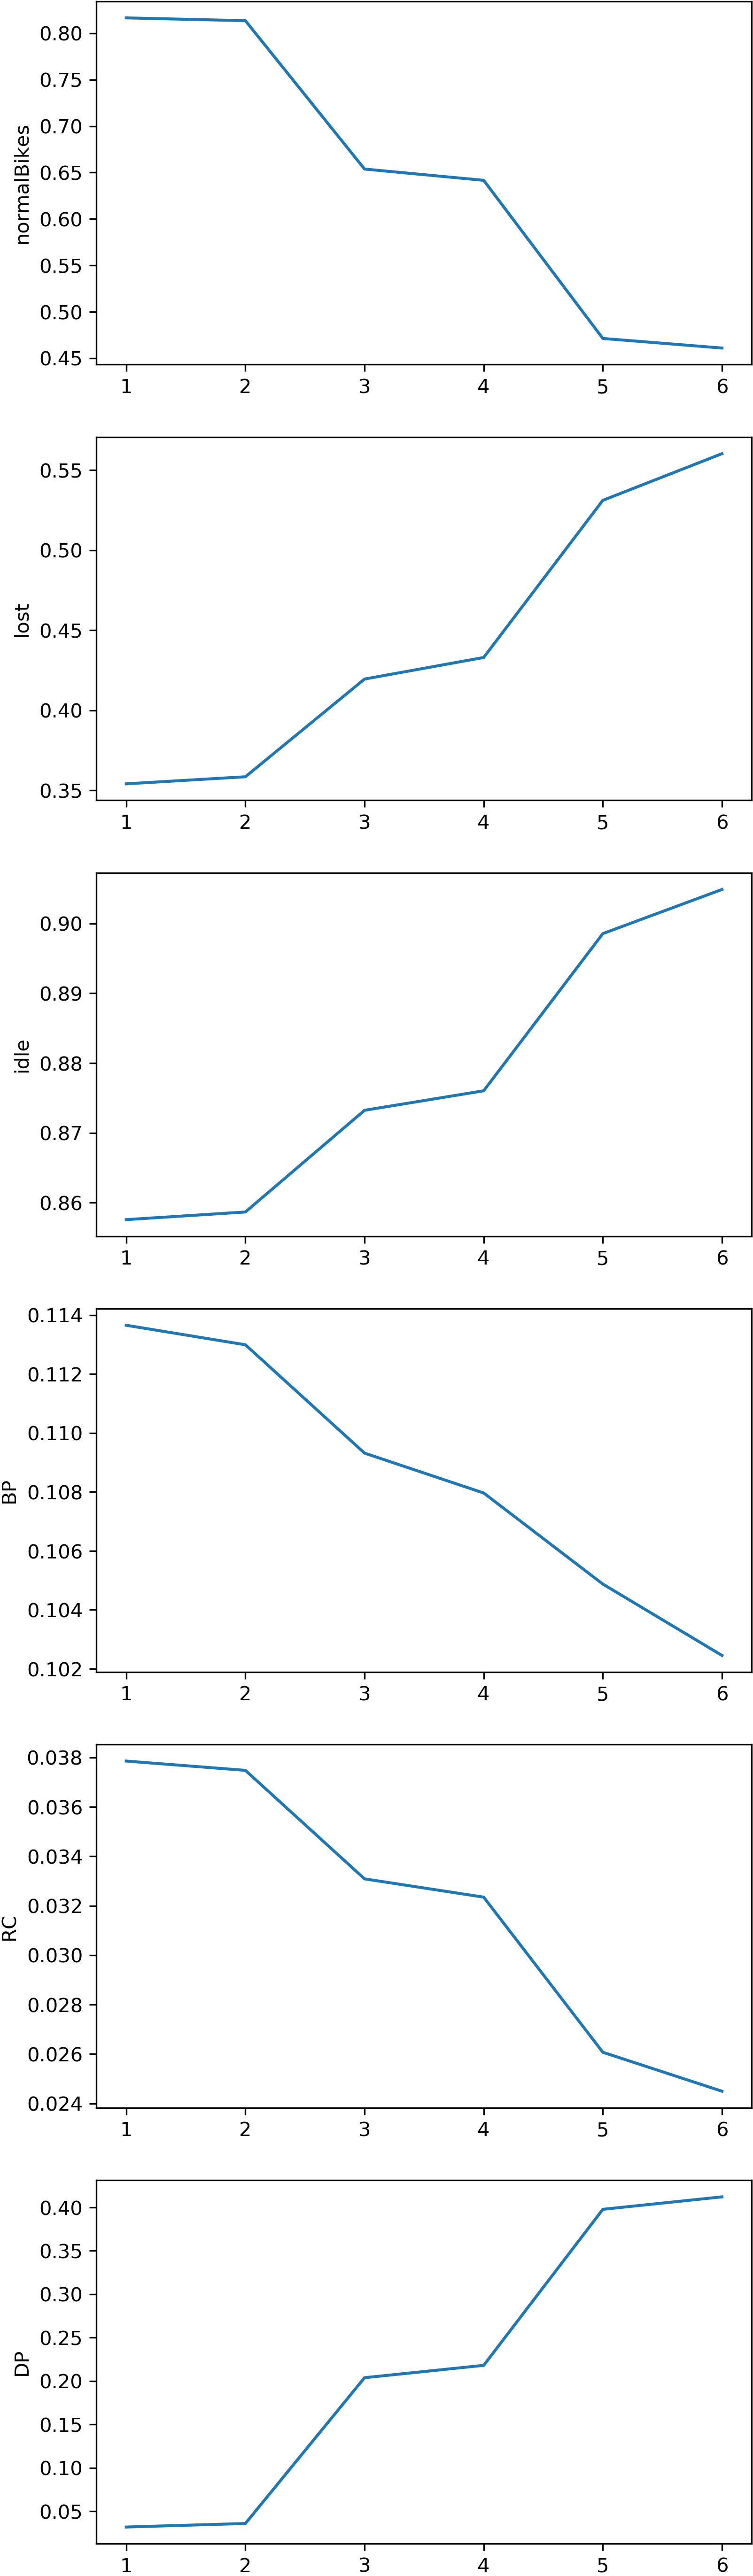
\includegraphics[width=2.3in]{Graph/perfD_1-6.png}
%     %\caption{fig2}
%     \end{minipage}%
%     }%
% \end{figure}
% \restoregeometry